\chapter{Introduction}

Signal processing is a field which often interweaves pure mathematics and engineering. One of its concerns is the \textit{representation} of signals (functions) and how different representations may be explored to better manipulate such signals. The spectral analysis via Fourier and similar transforms, for instance, aims to project the signal onto a domain in which the energy support is more compact (compression), or in which some frequencies are easier to be removed (filtering), or yet in which some relevant features may be created (feature engineering for machine learning problems), among others \cite{oppenheim1999discrete, rabiner2010theory, graf2015features, vergin1999generalized}.

One way to explore different signal representations is to alter the algebra over which it is defined. That is the case with numerical or arithmetic transforms \cite{blahut2010fast,pedrouzo2017number,chandra2014exact}, which deal only with finite fields instead of the usual complex (e.g. Fourier transform) or real fields (e.g. cosine transform). As the underlying algebra is extended, e.g. going from $ \mathbb{R} $ to $ \mathbb{C} $, it is possible to process signals with more information per sample. Such was the motivation behind Sangwine's \cite{sangwine1996fourier} discrete version of a family of bidimensional transforms over the \textit{quaternions}, previously created by Ell \cite{ell1993quaternion}: to exploit this class of hypercomplex numbers with four real components to perform holistic color image processing. Upon mapping each color channel inside a pixel into an imaginary component of a quaternion number, the color image may be processed as a single signal. Computationally, the spectral decomposition requires only two complex discrete Fourier transforms (DFTs), instead of three (one per color channel). Ever since, quaternion transforms have been employed not only on color image processing \cite{ell2007hypercomplex,chen2018quaternion,li2013quaternion,evans2000hypercomplex}, but also other ends such as bivariate signal analysis \cite{flamant2017spectral,flamant2017time,flamant2018complete}.

Algebra extensions change the signal representation by looking at the signal \textit{samples} but, reminding the signal is nothing more than a function, one may also shift the attention to the \textit{domain}. In fact, such reflection has led to the creation of graph signal processing (GSP). This field, which emerged in the last decade, is concerned with extending the concepts of classical discrete signal processing (DSP) to the in which the signal samples \textit{reside in graph vertices}. It approaches the classical case of discrete-time domain as being a path or ring graph -- depending on the graph shift operator (GSO) at hand, as will soon be clear -- with equally weighted edges. The \textit{signal}, therefore, is a mapping from the vertex set to the real (or complex) numbers, and the fixed sampling frequency is represented as graph edges having the same weights (i.~e. as if the samples were at fixed ``distances'', one could say). GSP deals with the consequences of conecting more vertices in this graph, moving from the queue-shaped domaing into an arbitrary network. Many definitions from classical DSP have already found their way into GSP, thanks to the contributions of many scholars who proposed ways to implement filtering \cite{sandryhaila2013filters}, linear transforms \cite{sandryhaila2013gft,sardellitti2017graph}, interpolation \cite{segarra2015interpolation}, sampling theorem on graphs \cite{wang2015generalized,chen2016signal,tsitsvero2016signals}, among others.

The endeavour to experiment with different algebras or domain topologies has primarily theoretical motivations, but often reveal new solutions to real world problems. Taking GSP for instance, its applications spread from coding \cite{su2017graph} and light-field image super resolution schemes \cite{rossi2017graph}, to regulatory genetic networks, in which graph-based methods improved three state-of-the-art network inference schemes \cite{pirayre2015brane,pirayre2017brane}, also reaching recommender systems, both collaborative filtering and content-based, using regularization of graph total variation \cite{benzi2016song}, semi-supervised learning through adaptive graph filters \cite{chen2014semi}, community detection using graph wavelets \cite{tremblay2014graph}, among others. The latter examples hint at the intersection between GSP and the fields of data science and machine learning -- well established and highly active, both in Academia and industry --, to the point where we can join Benjamin Ricaud and say that \emph{Fourier could very well be, today, a data scientist} \cite{ricaud2019fourier}.

As happened to GSP, the study of quaternion-valued signal processing has also found applications. Beyond the already mentioned use in manipulating color image and bivariate signals, the work on adaptive quaternion filters has been useful, for example, in wind profile prediction \cite{jiang2014general}. Or yet the remarkable union of graphs and quaternions in the work by \cite{zhang2019quaternion} -- the only one the author is aware of --, in which quaternion embeddings are used to form a low dimensional representation of entities and relations in knowledge graphs.

In this context, the current thesis aims to tackle the following problem: is it possible to perform signal processing having quaternion-valued samples residing on graphs with quaternion-weighted edges? What limitations and new possibilites may arise when exploring what we may call \textit{quaternion graph signal processing} (QGSP)? That is the spark which ignited the studies and results presented in the following chapters.

As will become clear to the reader, however, the pathway to the basis of QGSP was not a straight line. Sometimes what seemed to be dead ends emerged, and during the reflections upon ways to bypass them, other interesting results started to show themselves. For example, it was certain from the beginning that the problem of eigendecomposing quaternion matrices would be at the heart of QGSP, since the very definition of a graph signal spectrum requires the eigenvalues and eigenvectors of a GSO (e.g. the adjacency matrix), which is a quaternion matrix. Since it took a while to make progress with general graph matrices, it seemed promising to investigate the quaternion discrete Fourier transform (QDFT); after all, ring graphs should have the graph Fourier transform (GFT) and the classical discrete Fourier transform (DFT) coinciding. By looking at the QDFT matrix, however, a new way to diagonalize it was found and a new multiparametric fractional QDFT was proposed. When shifting the focus to the graph domain, revisiting the study of graph shift operators and their spectral decomposition, interesting results regarding the fractional GSO were discovered. For instance, this new operator acts as a graph filter, and its polynomial representation is determined, demonstrating that it can be implemented as a linear and shift-invariant (LSI) graph filter.

\section{Organization}

This thesis is organized as follows. Chapters \ref{ch:reviewQuat} and \ref{ch:reviewGSP} bring a diverse set of concepts and results from the literature, providing the reader with a sufficient understanding of the quaternion algebra and quaternion Fourier transform (the former), and signal processing from the perspective of graph signals and fractional-order operators (the latter).
Chapter \ref{ch:FrGSO} presents the new fractional graph shift operator, commenting on its properties and applications.
In Chapter \ref{ch:FrQDFT}, a study on the fractionalization of the QDFT is presented, with a new method being proposed, alongside a multiparametric version of the fractional-order transform.
The foundations of QGSP are finally presented in Chapter \ref{ch:QGSP}, with discussions and a few applications with both toy and real world datasets.
The thesis closes with concluding remarks and future works, in Chapter \ref{ch:conclusion}. The Appendix \ref{ch:AppendixA} leads the reader through the demonstration of a relation between systems of quaternion and complex linear equations, useful for a central theorem presented in Chapter \ref{ch:reviewQuat}.

\section{Contributions}
The contributions presented in this thesis are:

\begin{itemize}[noitemsep]
    \item The proposition and discussion of the fractional graph shift and its application on improving least-squares approximation of linear and shift-invariant ideal filters.
    \item A novel approach to fractionalizing the quaternion discrete Fourier transform (QDFT)
    \item The definition of a multiparametric fractional QDFT and its application in a novel image encryption scheme.
    \item The proposition of Quaternion Graph Signal Processing (QGSP), a new tool designed for specialized scenarios in which both the signal samples and their quantifiable relationship may be expressed as quaternions (thus having at most four dimensions or information sources).
    \item \texttt{gspx}\footnote{The library is available as an open repository: \url{https://github.com/gboaviagem/gspx}.}, an open-source Python library with implementation of the core concepts from QGSP.
\end{itemize}

\section{Publications}

This work has so far published two papers in international journals, one in a global conference, and a book. The paper \textit{``Eigenstructure and fractionalization of the quaternion discrete Fourier transform''}, published in Optik, contains the results of Chapter \ref{ch:FrQDFT}. The 10th volume of IEEE Access received the work \textit{``On the Fractionalization of the Shift Operator on Graphs''}, containing the results of Chapter \ref{ch:FrGSO}. As the understanding of GSP matured during the doctorate research, the author contributed with some chapters of the book ``Processamento de Sinais sobre Grafos: Fundamentos e Aplica{\c c}{\~o}es'', published in the \textit{Notas em Matem\'atica Aplicada} series from the Brazilian society \textit{Sociedade Brasileira de Matemática Aplicada e Computacional (SBMAC)}.

The paper \emph{``The Cosine Number Transform: A Graph Signal Processing Approach''}, presented in the 2019 edition of GlobalSIP, was created during short attempts to further generalize GSP to other algebraic structures, in particular to graphs with edge weights in finite fields. However, it has not evolved into more substantial findings and thus, although it stems from this work, it is not featured in this thesis. The full references of the mentioned publications are:

\begin{itemize}[noitemsep]
% Citing in MLA Format, extracted from Google Scholar.
\item Ribeiro, Guilherme and Lima, Juliano. ``The Cosine Number Transform: A Graph Signal Processing Approach''. \textit{2019 IEEE Global Conference on Signal and Information Processing (GlobalSIP)}. IEEE, 2019. DOI: \href{https://doi.org/10.1109/GlobalSIP45357.2019.8969165}{10.1109/GlobalSIP45357.2019.8969165}

\item Ribeiro, Guilherme B., and Lima, Juliano B. ``Eigenstructure and fractionalization of the quaternion discrete Fourier transform''. \textit{Optik} 208 (2020): 163957. DOI: \href{https://doi.org/10.1016/j.ijleo.2019.163957}{10.1016/j.ijleo.2019.163957}.

\item Ribeiro, Guilherme B., José R. De Oliveira Neto, and Lima, Juliano B. ``On the Fractionalization of the Shift Operator on Graphs''. \textit{IEEE Access} 10 (2022): 16468-16478. DOI: \href{https://doi.org/10.1109/ACCESS.2022.3149755}{10.1109/ACCESS.2022.3149755}.

\item Lima, Juliano, et al. \textit{Processamento de Sinais sobre Grafos: Fundamentos e Aplica{\c c}{\~o}es}. Notas em Matem\'atica Aplicada, v. 92. Sociedade Brasileira de Matemática Aplicada e Computacional (SBMAC), 2022.
\end{itemize}

% O escopo desta pesquisa orbita, essencialmente, a aplica\c c\~ao de matrizes quaterni\^onicas no contexto de processamento de sinais. Sejam matrizes de adjac\^encia de grafos, ou matrizes de transforma\c c\~oes lineares quaterni\^onicas, o entendimento de sua autoestrutura e a interpreta\c c\~ao correta de opera\c c\~oes que delas fazem uso s\~ao os fios condutores desta tese. O objetivo geral consiste em expandir as ferramentas da literatura em processamento de sinais quaterni\^onicos, particularmente aplicando a grafos de pesos quaterni\^onicos, e propor novas interpreta\c c\~oes e cen\'arios de aplica\c c\~ao.

% Os objetivos espec\'ificos a serem alcan\c cados s\~ao
% \begin{itemize}[noitemsep]
% \item o estudo da fracionariza\c c\~ao da transformada discreta de Fourier quaterni\^onica (QDFT, \emph{quaternion discrete Fourier transform}),
% \item expandindo o item anterior, pretende-se avan\c car no estudo de diagonaliza\c c\~ao de matrizes quaterni\^onicas e
% \item investigar cen\'arios modelados por grafos com pesos quaterni\^onicos, bem como as dificuldades alg\'ebricas ou computacionais oriundas da n\~ao-comutatividade dos quat\'ernios.
% \end{itemize}

\section{Notation}
The use of symbols is a great way to communicate ideas concisely. However, instead of improving communication, they may make it cumbersome or even not communicate at all if the reader is not adequately familiar with them. Let us go through the main notation in this thesis, to avoid confusion instead of clarity.

Simple numbers, either real-, complex- or quaternion-valued, are represented in italics, as in $q$. Numerical sets (and the related fields or skew-fields) are denoted using blackboard bold face (such as $\mathbb{R}$). Vectors and matrices are written with bold face: the former with lower case ($\mathbf{v} \in \mathbb{R}^{n}$), and the latter with upper case ($\mathbf{V} \in \mathbb{R}^{n \times n}$).

The function $\mathrm{diag}(\cdot)$ has context-dependent meaning: when the argument is a matrix, it returns the main diagonal as a column vector; whereas when it is a vector, it produces a diagonal matrix with this vector in its main diagonal.


\chapter{A review on quaternion algebra and its Fourier transform}
\label{ch:reviewQuat}

\begin{quotation}
\itshape
And here there dawned on me the notion that we must admit, in some sense, a fourth dimension of space for the purpose of calculating with triples... An electric circuit seemed to close, and a spark flashed forth.

\noindent --- Sir William Hamilton.
\end{quotation}


In 1833, at the age of 28, Willian Rowan Hamilton presented to the Royal Irish Academy (RIA) a work in which complex numbers were treated as ordered pairs of real numbers, given the appropriate definition of operations\footnote{The results were published in 1837, in the paper \emph{Theory of Conjugate Functions, or Algebraic Couples; with a Preliminary and Elementary Essay on Algebra as the Science of Pure Time} \cite{hamilton1837theory}.}. In the following years, he struggled to extend the complex field into a normed division algebra ober triples, but soon realized that, as much as his attempts were inventive, the resulting algebra was not closed under multiplication. We can see this through a simple example \cite{santos2011algebra}: let it be the set $\mathbb{F} = \{ a + b \qi + c \qj  \ | \ (a, b, c) \in \mathbb{R}^3\}$, with $\qi^2 = \qj^2 = -1$ and $\qi \neq \qj$. Since $\qi, \qj \in \mathbb{F}$, so there must exist $x, y, z \in \mathbb{R}$ so that
\begin{equation}
\qi \qj = x + y \qi + z \qj.
\label{eq:demonstration01}
\end{equation}

Multiplying by $\qi$ both sides of the equation,
\begin{equation}
\qi^2 \qj = \qi x + \qi^2 y + z (\qi \qj),
\end{equation}
and using (\ref{eq:demonstration01}) it yields,
\begin{equation}
- \qj = \qi x - y + z (x + y \qi + z \qj)
\Rightarrow
(zx - y) + \qi (x + zy) + \qj (z^2 + 1) = 0.
\end{equation}
That is: $z \notin \mathbb{R}$ and $ \qi \qj \notin \mathbb{F} $, proving that such algebraic structure is not closed under multiplication.

Only a decade later, in 1843, while walking by the roads in Dublin towards the RIA, ``an electric circuit seemed to close, and a spark flashed forth'', as he would say. He had conceived the four-dimensional structure required to the desired algebra, creating the quaternions. Moved by excitement, he craved on the stone below Broome Bridge, in Cabra (Dublin), the equations that define the relations between the canonical basis elements of quaternions\footnote{Close to the original site of the inscriptions, the RIA placed a commemorative plaque in 1958, with the same writings.}. This creation, made possible by an insight in 1843, is found accross most of this work. The following sections lead the reader through the foundations of quaternion algebra and quaternion signal processing.


\section{Introduction to the quaternion algebra}

Quaternions are numbers $q \in \mathbb{H}$ in the form
\begin{equation}
q = a + b\qi + c\qj + d\qk,
\label{eq:q}
\end{equation}
in which $a, b, c, d \in \mathbb{R}$, holding true the fundamental relations:
\begin{equation}
\label{eq:fund_rel}
\begin{aligned}
\qi ^2 = \qj^2 &=\qk^2 = \qi \qj \qk = -1.
\end{aligned}
\end{equation}

The multiplication rules between  $ \qi $, $ \qj $ and $ \qk $ follow directly from (\ref{eq:fund_rel}), resembling those between orthonormal basis vectors from $ \mathbb{R}^3 $: the product between two of them yields the third, the sign being determined from the operands order. For instance, to find the result of $ \qi \qj $ one may start from (\ref{eq:fund_rel}) and write
\begin{equation}
\begin{aligned}
\qi \qj \qk &= -1 \\
\qi \qj \underbrace{\qk \qk}_{= -1} &= -\qk \\
\qi \qj &= \qk.
\end{aligned}
\end{equation}
Similarly, to find $ \qj \qi $,
\begin{equation}
\begin{aligned}
\qi \qj \qk &= -1 \\
\qi \qi \qj \qk &= -\qi \\
- \qj \qk &= - \qi \\
\qj \qj \qk &=  \qj \qi \\
- \qk &=  \qj \qi. \\
\end{aligned}
\end{equation}
Figure \ref{fig:quatmult} depicts the order in which the product between two elements of the canonical basis yields the third, with positive sign. The most relevant consequence, therefore, of (\ref{eq:fund_rel}), is that the quaternion product is \textit{noncommutative}. In fact, it is the first noncommutative normed division algebra in history \cite{kleiner2007history}.

\begin{figure}
	\centering
	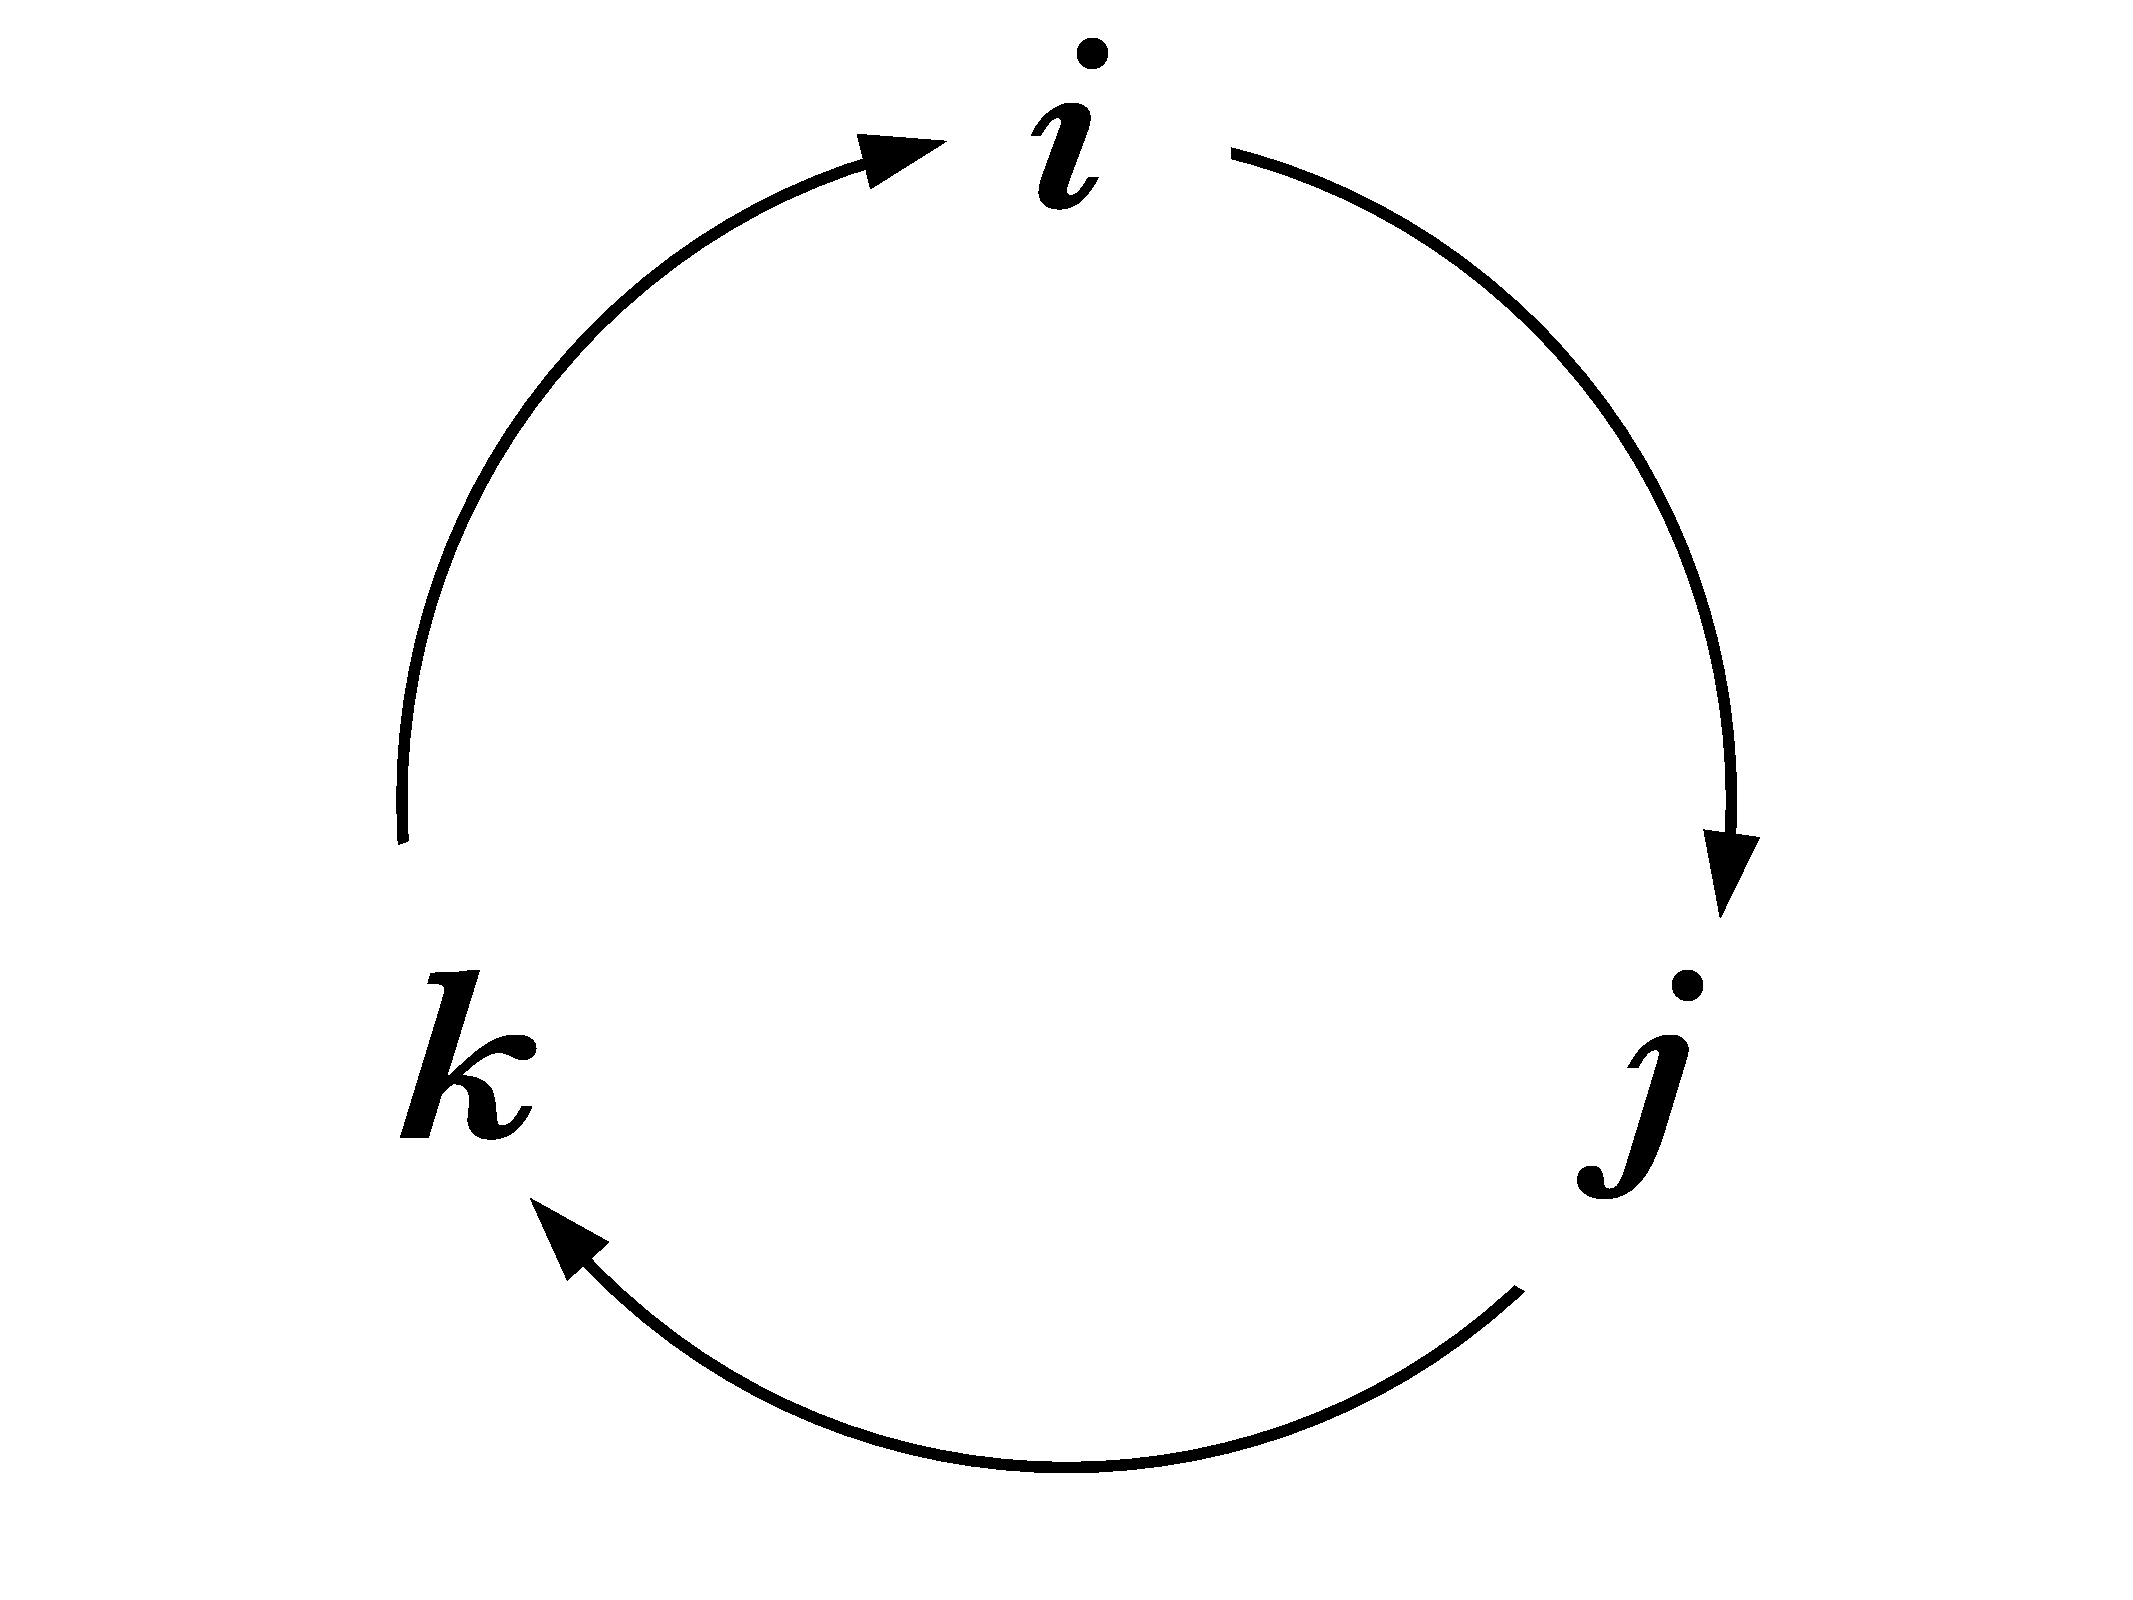
\includegraphics[width=0.2\linewidth]{Figures/quaternion_multiplication.pdf}
	\caption{Illustration of the multiplicatione rule between the imaginary units $ \qi $, $ \qj $ e $ \qk $.}
	\label{fig:quatmult}
\end{figure}

The exploration of the quaternion multiplication rules gives rise to a useful property, related to products between complex numbers and elements from the quaternion canonical basis. In particular, the product between $\qj$ and any complex number $x = a + b \qi , \ a, b \in \mathbb{R}$, satisfies $\qj x = \overline{x} \qj$, since
\begin{equation}
\label{eq:commutej}
\begin{aligned}
\qj x &= \qj (x_r + x_i \qi) = x_r \qj + x_i \qj \qi = x_r \qj - x_i \qi \qj \\
&= (x_r - x_i \qi) \qj = \overline{x} \qj.
\end{aligned}
\end{equation}
This will come up a couple of times during manipulations in this thesis.

The elements $\qi, \qj$ e $\qk$ may be perceived as orthogonal imaginary units, generating the 3D space of quaternion \textit{imaginary parts},
\begin{equation}
\qV (q) = b\qi + c\qj + d\qk.
\end{equation}
The \emph{real part} of a quaternion \emph{q} is defined as
\begin{equation}
S(q) = a.
\end{equation}

The imaginary part is usually referred to as \textit{vector part}, while the real part may also be called \textit{scalar part}. A quaternion with null real part is said to be \textit{pure} --- the set of which is represented by $\qV(\mathbb{H})$. The product between pure quaternions may be written similarly to that between $\mathbb{R}^3$ vectors, i.~e. if $v_1 = b_1\qi + c_1\qj + d_1\qk$ and $v_2 = b_2\qi + c_2\qj + d_2\qk$, then
\begin{equation}
v_1 \times v_2 = 
\begin{vmatrix}
\qi & \qj & \qk\\ 
b_1 & c_1 & d_1\\ 
b_2 & c_2 & d_2
\end{vmatrix}.
\end{equation}

Based on the similarity between the $ \mathbb{R}^3 $ set, equipped with the cross product, and the set of pure quaternions, equipped with their quaternion product, it is usual to refer to $\qi, \qj$ and $\qk$ as \emph{axis}. The term references the interpretation of theses imaginary units as being coordinate axis in the 3D space of pure quaternions.

The analogy with the $\mathbb{R}^3$ vector operations also extends to the definition of inner product between pure quaternions $v_1 = b_1\qi + c_1\qj + d_1\qk$ and $v_2 = b_2\qi + c_2\qj + d_2\qk$:
\begin{equation}
\langle v_1, v_2 \rangle =
b_1 b_2 + c_1 c_2 + d_1 d_2.
\end{equation}

The quaternion multiplication distributes over quaternion addition
% this english sentence is right: https://en.wikipedia.org/wiki/Distributive_property
and is also associative. That is, if $q_1 = a_1 + b_1\qi + c_1\qj + d_1\qk$ and $q_2 = a_2 +  b_2\qi + c_2\qj + d_2\qk$, then their sum is simply
\begin{equation}
q_1 + q_2 = (a_1 + a_2) + (b_1 + b_2)\qi + (c_1 + c_2)\qj + (d_1 + d_2)\qk,
\end{equation}
whereas their product is
\begin{equation}
\label{eq:q_prod}
\begin{aligned}
q_1 q_2 = &  \ (a_1 + b_1\qi + c_1\qj + d_1\qk) (a_2 +  b_2\qi + c_2\qj + d_2\qk)  \\
= & \ (a_1 a_2 - b_1 b_2 - c_1 c_2 - d_1 d_2)  \\
& + \qi (b_1 a_2 + a_1 b_2 - d_1 c_2 + c_1 d_2)  \\
& + \qj (c_1 a_2 + d_1 b_2 + a_1 c_2 - b_1 d_2)  \\
& + \qk (d_1 a_2 - c_1 b_2 + b_1 c_2 + a_1 d_2).
\end{aligned}
\end{equation}

Finally, it is possible to write the quaternion product in (\ref{eq:q_prod}) as a function of the operands scalar and vector parts,
\begin{equation}
\label{eq:prod_vectors}
\begin{aligned}
q_1 q_2 = & \ S(q_1)S(q_2) - \langle\qV(q_1), \qV(q_2)\rangle \\
& + S(q_1) \qV(q_2) + S(q_2)\qV(q_1) + \qV(q_1) \times \qV(q_2).
\end{aligned}
\end{equation}
The lack of commutativity in the cross product is another demonstration of the fact that quaternion multiplication is noncommutative.

Quaternion conjugation, as defined in the complex numbers, is obtained changing the sign of the imaginary part: $ \bar{q} \overset{\Delta}{=} S(q) - V(q) $. The quaternion \textit{norm} is defined as $\Vert q \Vert \overset{\Delta}{=} a^2 + b^2 + c^2 + d^2 = q \bar{q} = \bar{q} q$, whereas the \textit{modulus} of $q$ \cite{ell2014quaternion} is
\begin{equation}
\label{eq:modulusq}
|q| \overset{\Delta}{=} \sqrt{a^2 + b^2 + c^2 + d^2} = \Vert q \Vert^{\nicefrac{1}{2}}.
\end{equation}

A \textit{unit} quaternion has, by definition, unit norm, and the norm definition also leads to the quaternion multiplicative inverse,
\begin{equation}
q^{-1} = \frac{\bar{q}}{\Vert q \Vert}.
\end{equation}

From the analogy between pure quaternions and the elements in $ \mathbb{R}^3 $, the idea of perpendicularity between pure quaternions presents itself naturally. Given $ \qmu,  \qnu \in \qV(\mathbb{H})$, they are said orthogonal --- we write $ \qmu \perp \qnu $ --- if and only if
\begin{equation}
S(\qmu \qnu) = \langle \qmu, \qnu \rangle = 0.
\tag{$ \iff \qmu \perp \qnu $}
\end{equation}
For two orthogonal unit pure quaternions $ \qmu $ and $ \qnu $, it follows from (\ref{eq:prod_vectors}) that $ \qmu \qnu  = \qmu \times \qnu$, therefore $ \qmu \qnu \perp \qmu $ and $ \qmu \qnu \perp \qnu $. Since $ (\qmu, \qnu, \qmu \qnu) $ is a triplet of orthogonal pure unit quaternions, they form a basis for $ \qV (\mathbb{H}) $. Hence it is possible to rewrite (\ref{eq:q}) as
\begin{equation}
\label{eq:quat_generalizado}
q = a + b'\qmu + c'\qnu + d'\qmu \qnu,
\end{equation}
$a, b', c', d' \in \mathbb{R}$,
which represents the so called \emph{generalized quaternion}. The \emph{classical Hamiltonian quaternions} are those written in terms of the canonical basis $ (1, \qi, \qj, \qk) $.


Besides the cartesian representation (\ref{eq:q}), quaternions allow the so called \emph{Euler form} \cite{ell2014quaternion}, a polar representation commonly expressed as
\begin{equation}
\label{eq:euler}
q = |q| e^{\qmu \theta} = |q|\cos \theta + |q|\qmu \sen \theta,
\end{equation}
in which $ \qmu $ is a pure unit quaternions, parallel to the vector part of $ q $.

As a remarkable consequence of (\ref{eq:euler}), it follows that every pure unit quaternion is a square root of $-1$. For instance, let $ \qnu $ be a unit pure quaternion. From (\ref{eq:euler}),
\begin{equation}
%\label{key}
\qnu = |\qnu| e^{\qnu \theta},
\end{equation}
but since $ |\qnu| = 1 $, then
\begin{equation}
%\label{key}
\qnu = e^{\qnu \theta}  = \cos \theta + \qnu \sen \theta \Rightarrow \theta = \frac{\pi}{2},
\end{equation}
hence,
\begin{equation}
%\label{key}
\qnu^2 = \left( e^{ \qnu \frac{\pi}{2}} \right)^2 = e^{\qnu \pi} = \cos \pi + \qnu \sen \pi = -1.
\end{equation}

This property leads to the conclusion that numbers such as $ a + \qmu b  $ form an isomorphism with the complex numbers. For this reason, the set composed by such numbers is represented by $ \mathbb{C}_{\qmu} \overset{\Delta}{=} \{ a + \qmu b \ |\  a, b \in \mathbb{R} \}$ (hence $ \mathbb{C}_{\qi} $ indicates the usual set of complex numbers).

Another crucial representation of quaternion numbers is called \emph{symplectic decomposition}. Every quaternion $ q = a + b\qi + c\qj + d\qk \in \mathbb{H} $ can be represented as
\begin{equation}
q = q^{(s)} + q^{(p)} \qj, \quad q^{(s)}, q^{(p)} \in \mathbb{C}_{\qi},
\end{equation}
in which the complex numbers $ q^{(s)} = a + b\qi $ and $ q^{(p)} = c + d\qi $ are commonly named \emph{simplex} and \emph{perplex} parts, respectively. In general, the decomposition does not need to take $\qi$ as reference axis. Take for example $ \qmu $ and $ \qnu $ as arbitrary orthogonal unit pure quaternions, hence any quaternion $ q $ may be decomposed as
\begin{equation}
\label{eq:decomposicao}
q = q^{(s)} + q^{(p)} \qnu, \quad q^{(s)}, q^{(p)} \in \mathbb{C}_{\qmu}.
\end{equation}
That is a hugely important tool when it comes to computing the QDFT (see Section \ref{sec:QFT}) and handling quaternion matrices (cf. Chapter \ref{ch:QGSP}).

\subsection{Quaternion similarity and rotation}
\label{subsec:rotacionando}
Two quaternions $ q $ and $ r $ are said to be \emph{similar} if it exists a non-zero quaternion $ v $ such that $ v^{-1}q v = r $. In this case, one can write $ q \sim r $. Similarity between quaternions constitutes an equivalence relation \cite{zhang1997quaternions}, and all elements from a same similarity class possess the same norm, since $ |v^{-1}q v| = |v^{-1}| \cdot |q| \cdot |v| = |q| $.

It matters to notice that an important property of quaternion similarity transformations, which justifies its great use in mechanics and graphics computing industry, is that it performs a rotation on the $\qi \qj \qk$ space. Given $ v,x \in \mathbb{H} $, $ v = |v| e^{\qmu \alpha}$, the similarity transformation
\begin{equation}
\label{eq:rotacao}
\phi_v(x) = v x v^{-1}
\end{equation}
produces the rotation of the vector part of $x$ along the axis $ \qmu $ (which is parallel to the vector part of $v$) through an angle $ 2\alpha $ \cite{ward2012quaternions}, following the right-hand rule. Let us illustrate this property with an example.

\vspace{-2em}
\begin{quotation}
\begin{example}
\label{example:01}
\upshape
Let $ \lambda = 3\qi + \qk $ and
\begin{equation}
%\label{key}
\mathbf{v} =\begin{pmatrix}
1 +  \qi\\
2 \qj + \qk
\end{pmatrix}
\end{equation}
be, respectively, an eigenvalue and its eigenvector of a matrix $\mathbf{A} \in \mathbb{H}^{2 \times 2}$. The eigenvalue problem over the quaternions will be introduced in the next section, so let us not consider its details for now. It suffices to know that $\lambda$, $\mathbf{A}$ and $\mathbf{v}$ satisfy the equation
\begin{equation}
\label{eq:03}
\mathbf{A} \mathbf{v} = \mathbf{v} \lambda.
\end{equation}

Let us restrict the first column of $\mathbf{A}$ to be equal to $ (1 \quad 1)^T $, so that the the matrix is now fully determined,
\begin{equation}
%\label{key}
\mathbf{A} =
\begin{pmatrix}
1 & - \frac{1}{5} + \frac{3}{5} \qi + 2 \qj \\
1 & -3 \qi + \qj
\end{pmatrix}.
\end{equation}

Given an invertible quaternion $q$, the equation may be rewritten as
\begin{equation}
\label{eq:rewritten}
\mathbf{A} (\mathbf{v} q) = (\mathbf{v} q) q^{-1} \lambda q,
\end{equation}
which presents the similarity transformation $q^{-1} \lambda q$. Since similar quaternions differ only by a rotation of their vector parts, it is clearly possible to find a quaternion $q$ so that the vector part of $q^{-1} \lambda q$ is parallel to $\qi$ --- that is, $q^{-1} \lambda q$ is a complex number. Let us go through that process.

Since the vector part of $\lambda$ belongs to the $ \qi \qk $ plane, the idea is to use (\ref{eq:rotacao}) to rotate $\lambda$ along the $\qj$ axis (orthogonal to the rotation plane) by an angle of $ \theta = \tan^{-1} \frac{1}{3} $ radians, towards $ \qi $ (see Fig. \ref{fig:quat3ik}). The required quaternion to enable such rotation is, therefore,
\begin{equation}
\label{eq:04}
v = e^{\qj \alpha}, \quad 2\alpha = \theta = \tan^{-1} \frac{1}{3},
\end{equation}
using the mapping $ \lambda \mapsto v \lambda v^{-1} $ in (\ref{eq:rotacao}).

\begin{figure}
\centering
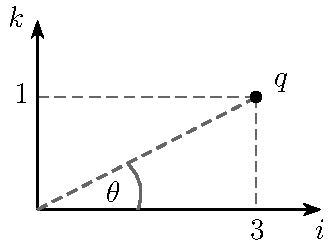
\includegraphics[width=0.25\linewidth]{Figures/quaternion01.pdf}
\caption{Representation of $ \lambda = 3\qi + \qk $ in the $ \qi \qk $ plane.}
\label{fig:quat3ik}
\end{figure}

Recalling that our desired transformation is written as $ \lambda \mapsto q^{-1} \lambda q $, then
\begin{equation}
%\label{key}
q = v^{-1} = e^{- \qj \alpha} = e^{- \qj \frac{\theta}{2}}.
\end{equation}

As a sanity check, let us find the value of $ \alpha $ which results in $ q^{-1} \lambda q \in \mathbb{C}_{\qi} $. Since $ v = q^{-1} = \cos \alpha + \qj \sin \alpha $,
\begin{equation}
%\label{key}
\begin{aligned}
%\label{key}
q^{-1} \lambda &= (\cos \alpha + \qj \sin \alpha)(3 \qi + \qk)\\
&= \qi(3 \cos \alpha + \sin \alpha) + \qk(\cos \alpha - 3 \sin \alpha). \\
q^{-1} \lambda q &= [\qi(3 \cos \alpha + \sin \alpha) + \qk(\cos \alpha - 3 \sin \alpha)] (\cos \alpha - \qj \sin \alpha) \\
&= \qi (3 \cos 2\alpha + \sin 2\alpha) + \qk(\cos 2\alpha - 3 \sin 2\alpha).
\end{aligned}
\end{equation}

Therefore, $ q^{-1} \lambda q \in \mathbb{C}_{\qi} $ if and only if
\begin{equation}
%\label{key}
\begin{aligned}\textbf{}
\cos 2\alpha - 3 \sin 2\alpha &= 0 \\
2\alpha &= \tan^{-1} \frac{1}{3},
\end{aligned}
\end{equation}
as determined by (\ref{eq:04}).

Consequently, the unit pure quaternion $ q = e^{- \qj \alpha} $, $ \alpha = - \displaystyle \nicefrac{1}{2} \tan^{-1} \nicefrac{1}{3} $, yields $ q^{-1} \lambda q \in \mathbb{C}_{\qi}$, so that (\ref{eq:03}) can be rewritten as in (\ref{eq:rewritten}),
\begin{equation}
%\label{key}
\mathbf{A} \underbrace{\begin{pmatrix}
cos \alpha + \qi \sin \alpha - \qj \sin \alpha - \qk \sin \alpha \\
2 \sin \alpha + \qi \sin \alpha + \qj 2 \cos \alpha + \qk \cos \alpha
\end{pmatrix}}_{= \mathbf{v} q} =
(\mathbf{v} q) \cdot \underbrace{\qi (3 \cos 2\alpha + \sin 2\alpha)}_{= q^{-1} \lambda q}.
%\underbrace{3.162 \qi}_{= \bar{u} q u}.
\end{equation}
Let us leave a remark for the user, as an anticipation of the upcoming Section: notice how $\mathbf{v}$ and $\mathbf{v}q$ are the same eigenvector up to a scaling factor, and it is always possible to make $q^{-1} \lambda q$ a complex number, given that the vector part of $\lambda$ has non-zero norm.
\end{example}
\end{quotation}


\section{On the theory of quaternion matrices}

When analyzing the eigenstructure and subsequent fractionarization of the QDFT matrix, the eigendecomposition of the DFT and the eigenvector sharing served as a convenient shortcut. In order to build the results in QGSP, however, it is required to dive into more general properties of quaternion matrices. The symplectic decomposition, already presented in (\ref{eq:decomposicao}), plays an important role in that matter, specialy for its use in defining the \textit{complex adjoint matrix}.

\begin{definition}[Complex adjoint matrix \cite{zhang1997quaternions}]
\label{def:complexadjoint}
Given $ \mathbf{A} \in \mathbb{H}^{n \times n} $, with symplectic decomposition $ \mathbf{A}_1 + \mathbf{A}_2 \qj$, $ \mathbf{A}_1,\mathbf{A}_2 \in \mathbb{C}^{n \times n} $, its complex adjoint matrix is defined as
\begin{equation}
\rchi_{A} \overset{\Delta}{=}
\begin{pmatrix}
\mathbf{A}_1 & \mathbf{A}_2\\ 
- \overline{\mathbf{A}}_2 & \overline{\mathbf{A}}_1
\end{pmatrix}.
\end{equation}
\end{definition}

In the following theorems, Zhang brings fundamental results for building QGSP.

\begin{theorem}[Part of Theorem 4.2 in
\cite{zhang1997quaternions}
]
\label{th:equiv01}
Given the matrix $ \mathbf{A} \in \mathbb{H}^{n \times n} $, the following sentences are equivalent:

\begin{itemize}[noitemsep]
\item $ \rchi_{AB} = \rchi_{A} \rchi_{B} $,
\item $ \rchi_{A^{-1}} = \rchi_{A}^{-1}$, if $ \mathbf{A}^{-1} $ exists,
\item $ \rchi_{A}$ is unitary, Hermitian or normal if and only if so is $ \mathbf{A} $.
\end{itemize}

\end{theorem}

\begin{theorem}[Part of Theorem 4.3 in
\cite{zhang1997quaternions}
]
\label{th:equiv02}
Given the matrix $ \mathbf{A} \in \mathbb{H}^{n \times n} $, the following sentences are equivalent:

\begin{itemize}[noitemsep]
\item $\mathbf{A}$ is invertible.
\item $\mathrm{det}(\rchi_A) \neq 0$, i.e. $\rchi_{A}$ is invertible.
\end{itemize}

\end{theorem}

Differently from other representations of quaternion matrices in $ \mathbb{C} $ or $ \mathbb{R} $, the complex adjoint allows to establish an important relation between the spectra of $ \rchi_{A} $ and $ \mathbf{A} $, as will soon be discussed.

\subsection{Eigenvalues}
Since quaternion multiplication is noncommutative, it is necessary to distinguish between \textit{left} and \textit{right} eigenvalues of a given matrix $ \mathbf{A} \in \mathbb{H}^{n \times n} $,
\begin{align*}
\mathbf{A} \mathbf{v} &= \mathbf{v} \lambda, \tag{right} \\
\mathbf{A} \mathbf{v} &= \lambda \mathbf{v}.  \tag{left}
\end{align*}

We will restrict this discussion mostly to right eigenvalues, since they hold a broader set of results in literature \cite[Cap. 5]{zhang1997quaternions} and are, for that matter, a safer point of support when developing QGSP. When not explicitly mentioned, the right eigenvalues will simply be referred to as \textit{eigenvalues} of the quaternion matrix.

It matters to highlight the fact that a quaternion matrix possesses a \textit{finite} number of eigenvalues if and only if they are all real-valued. Otherwise, each of them will belong to a similarity class, according to the transformation $ \lambda_1 = q^{-1} \lambda_2 q $, containing \textit{infinite} quaternions which are also eigenvalues of the same matrix (return to Example \ref{example:01}, for instance). Let $ \lambda $ be an eigenvalue of the matrix $ \mathbf{A} $ associated with the eigenvector $ \mathbf{v} $. That is,
\begin{equation}
\begin{aligned}
\label{eq:similar}
\mathbf{A} \mathbf{v} &= \mathbf{v} \lambda \\
\mathbf{A} \mathbf{v} q &= \mathbf{v} \lambda q = \mathbf{v} q q^{-1} \lambda q \\
\mathbf{A} (\mathbf{v} q) &= (\mathbf{v} q) q^{-1} \lambda q,
\end{aligned}
\end{equation}
so that $ q^{-1} \lambda q $ is an eigenvalue associated with the eigenvector $ \mathbf{v}q $, with $ q \in \mathbb{H}^\ast $.

\subsection{Diagonalizability}
\label{subsec:autovetores_XA}

The problem of quaternion matrix diagonalization differs greatly from the case with complex matrices. In the latter scenario, having no pair of equal eigenvalues is a sufficient condition for diaginalizability, but the rule does not hold for the quaternio case. See for instance the counterexample given by Zhang \cite[Exemplo 7.4]{zhang1997quaternions}, the matrix
\begin{equation}
\mathbf{A} =
\begin{pmatrix}
\qi & 1\\ 
0 & \qj
\end{pmatrix}.
\end{equation}

Although its eigenvalues are distinct -- $ \qi $ and $ \qj $, since they lie on the main diagonal of an upper triangular matrix --, the respective eigenvectors do not constitute a linearly independent set. Notice, for example, that an eigenvector associated with $ \qi $ is $ (1, 0)^T $, whereas one associated with $ \qj $ is $ (\qi + \qj, 0)^T $. The reason as to why they form a linearly dependent set is the fact previously stated that, for each eigenvalue and eigenvector $ \lambda $ and $ \mathbf{v} $ from a quaternion matrix, it follows that $ q^{-1}\lambda q $ and $ \mathbf{v}q $ form another eigenvalue-eigenvector pair, with $ q \in \mathbb{H}^\ast $. That is, two \emph{similar} eigenvalues are always associated with the sample eigenvectors, up to a scaling factor. That is why similar quaternions are said to belong to the same \emph{eigenclass} \cite{de2000right}. In order to have a linearly independent set of eigenvectors, therefore, their eigenvalues must not be similar. Concluding the counterexample, the reader may show that $ \qi $ and $ \qj $ satisfy the similarity relation $ \qj = q \qi q^{-1} $ whenever $q$ belongs to the set $ \{ a - a\qi - a\qj + a\qk \ | \ a\in \mathbb{R}^\ast \} $.

Theorem \ref{th:02} relates the eigendecomposition of a quaternion matrix and that of its complex adjoint, providing a central principle to the study of quaternions matrices eigenstructure.

\begin{figure}
\centering
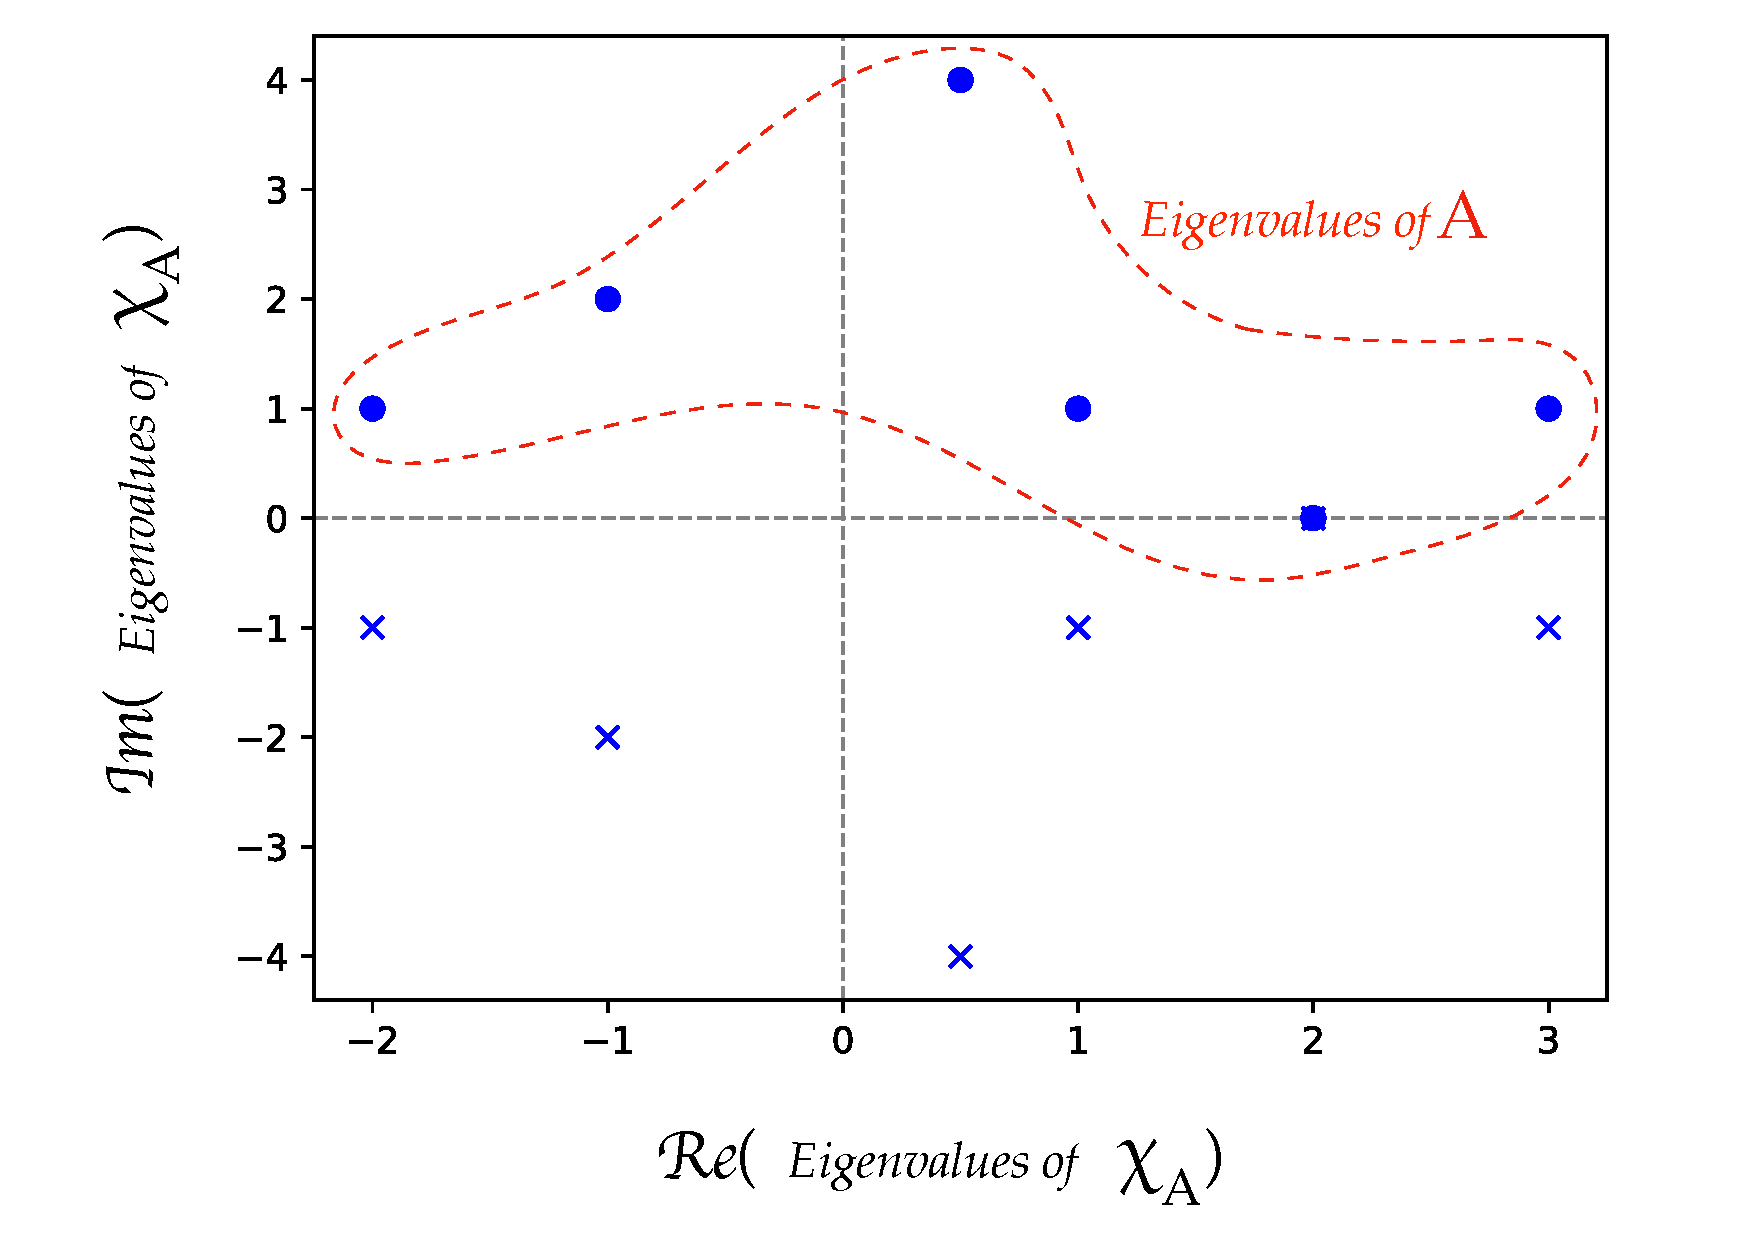
\includegraphics[width=0.6\linewidth]{Figures/complex_adjoint_eigvals_EN.pdf}
\caption{\emph{Standard eigenvalues} of a quaternion matrix $ \mathbf{A} $, indicated as a subset of the eigenvalues of the complex adjoint matrix.}
\end{figure}


\begin{theorem}[\cite{zhang1997quaternions}]
\label{th:02}
Every matrix $ A \in \mathbb{H}^{n \times n} $ has exactly $ n $ right eigenvalues which are complex numbers with nonnegative imaginary parts. These are called the \textbf{standard eigenvalues} of $ \mathbf{A} $ and are a subset of the $ 2n $ eigenvalues of $ \rchi_A $.
\end{theorem}

\begin{proof}
Como demonstrado no ap\^endice \ref{ch:AppendixA}, a partir da equa\c c\~ao de autovalor quaterni\^onica
\begin{equation}
\mathbf{A} \mathbf{v} = \mathbf{v} \lambda
\end{equation}
em que se pode assumir, sem perda de generalidade, que $ \lambda \in \mathbb{C} $, pode-se chegar \`a equa\c c\~ao equivalente
\begin{equation}
\label{eq:eigvalueequation}
\begin{pmatrix}
\mathbf{A}_1 & \mathbf{A}_2\\ 
- \overline{\mathbf{A}}_2 & \overline{\mathbf{A}}_1
\end{pmatrix}
\begin{pmatrix}
\mathbf{v}_1 \\ 
- \overline{\mathbf{v}}_2
\end{pmatrix} =
\begin{pmatrix}
\mathbf{v}_1 \\ 
- \overline{\mathbf{v}}_2
\end{pmatrix}
\lambda,
\end{equation}
envolvendo apenas vari\'aveis complexas (i.~e. as componentes da decomposi\c c\~ao de simpl\'etica de $ \mathbf{A} $ e $ \mathbf{v} $). Uma vez que
\begin{equation}
\rchi_A = 
\begin{pmatrix}
\mathbf{A}_1 & \mathbf{A}_2\\ 
- \overline{\mathbf{A}}_2 & \overline{\mathbf{A}}_1
\end{pmatrix}
\end{equation}
\'e uma matriz complexa $ 2n \times 2n $, ela possui $ 2n $ autovalores complexos (distintos ou não). Segundo \cite[Teorema 5]{lee1948eigenvalues}, seus autovalores ocorrem na forma de $ n $ pares conjugados e, por isso, a matriz $ \mathbf{A} $ possui exatamente $ n $ autovalores complexos com parte imagin\'aria n\~ao-negativa.

Os demais autovalores s\~ao redundantes. Seja $ q \in \mathbb{C}_{\qi}$ um destes autovalores. Podemos mostrar que $ q \sim \overline{q} $, pois obt\'em-se $ \overline{q} $ atrav\'es de uma rota\c c\~ao da parte imagin\'aria de $ q $ de 180$ ^\circ $ em torno do eixo $ \qj $. Utilizando o racioc\'inio exposto na subse\c c\~ao \ref{subsec:rotacionando}, com o quat\'ernio $ v = e^{\qj \frac{\pi}{2}} = \qj $ (logo $ v^{-1} = e^{- \qj \frac{\pi}{2}} = -\qj $) e o mapeamento $ q \mapsto v q v^{-1} $,
\begin{equation}
\begin{aligned}
v q v^{-1} &= \qj (q_r + q_i \qi) (-\qj) = q_r - q_i \qj \qi \qj\\
&= q_r + q_i \qi \qj \qj = q_r - q_i \qi = \overline{q}.
\end{aligned}
\end{equation}
Como dois autovalores conjugados de $ \rchi_A $ s\~ao similares, eles pertencem \`a mesma autoclasse e apontam para o mesmo conjunto linearmente dependente de autovetores. Assim, pode-se tomar sempre aquele com parte imagin\'aria nula ou n\~ao-negativa, por conven\c c\~ao.
\end{proof}

O teorema a seguir \'e outro resultado fundamental relacionando a autoestrutura de uma matriz quaterni\^onica e a de sua complexa adjunta.

\begin{theorem}[Teorema 7.4 em \cite{zhang1997quaternions}]
\label{th:diagonal}
Dadas as matrizes $ \mathbf{A}, \mathbf{B} \in \mathbb{H}^{n \times n} $, ent\~ao $ \mathbf{A} $ \'e similar a $ \mathbf{B} $ se, e somente se, $ X\rchi_A $ \'e similar a $ \rchi_B $.
\end{theorem}

\begin{corollary}
\label{cor:diagonalizable}
Uma matriz $  \mathbf{A} \in \mathbb{H}^{n \times n} $ \'e diagonaliz\'avel se, e somente se, $ \rchi_A $ \'e diagonaliz\'avel.
\end{corollary}
\begin{proof}
Se $ \mathbf{A} \in \mathbb{H}^{n \times n} $ \'e diagonaliz\'avel, ent\~ao \'e similar a uma matriz diagonal $ \Lambda \in \mathbb{C}^{n \times n}_{\qi} $ contendo seus autovalores padr\~ao. Do teorema \ref{th:diagonal}, segue que $ \rchi_A $ \'e similar a
\begin{equation}
\label{eq:Xlambda}
\rchi_{\Lambda} =
\begin{pmatrix}
\Lambda & \mathbf{0}\\ 
\mathbf{0} & \overline{\Lambda}
\end{pmatrix},
\end{equation}
que tamb\'em \'e uma matriz diagonal. Portanto, $ \rchi_A $ \'e diagonaliz\'avel.

Por outro lado, se $ \rchi_A $ \'e diagonaliz\'avel, ent\~ao \'e similar a uma matriz diagonal contendo os seus $ 2n $ autovalores, que aparecem em $ n $ pares complexos conjugados. Assim, sua matriz de autovalores pode ser escrita como (\ref{eq:Xlambda}), o que implica, pelo teorema \ref{th:diagonal}, que $ \mathbf{A} $ \'e similar a $ \Lambda $.
\end{proof}

\section{The quaternion Fourier transform}
\label{sec:QFT}

Ao considerar-se sinais de valores quaterni\^onicos, a literatura contempla algumas ferramentas para seu processamento, como um operador gradiente \cite{jiang2014general} e algoritmos de filtragem adaptativa \cite{jiang2013frequency}. Nesta se\c c\~ao, no entanto, o foco ser\'a dado \`a transformada de Fourier quaterni\^onica (QFT, \emph{quaternion Fourier transform}), base para a an\'alise espectral de fun\c c\~oes hipercomplexas.

Seja $f$ uma fun\c c\~ao de valores quaterni\^onicos $f: \mathbb{R} \rightarrow \mathbb{H}$ e $\qmu \in \qV(\mathbb{H})$, $\qmu^2 = -1$. A QFT unidimensional \emph{\`a esquerda} pode ser definida pela fam\'ilia de transformadas
\begin{equation}
\mathcal{F}^L_{\mp \qmu}[f](\omega) = 
F^L_{\mp \qmu}(\omega) \overset{def}{=}
\kappa_{-} \int_{-\infty}^{\infty} e^{\mp \qmu \omega t} f(t) \mathrm{d}t.
\tag{QFT 1D \`a esquerda}
\end{equation}

Pode-se provar que a opera\c c\~ao inversa existe e \'e dada por
\begin{equation}
\mathcal{F}^{-L}_{\pm \qmu}[F^L](t) = 
f(t) =
\kappa_{+} \int_{-\infty}^{\infty} e^{\pm \qmu \omega t} F^L(\omega) \mathrm{d}\omega.
\tag{QFT 1D \`a esquerda inversa}
\end{equation}

Nas express\~oes acima, o quat\'ernio puro unit\'ario $\qmu$ indica o \emph{autoeixo} do n\'ucleo da transformada, \'e a unidade imagin\'aria de refer\^encia. Seu sinal no n\'ucleo da transformada \'e arbitr\'ario, bastando que as transforma\c c\~oes direta e inversa contenham sinais opostos. As constantes reais $\kappa_{-}$ e $\kappa_{+}$ satisfazem
\begin{equation}
\kappa_{+} \kappa_{-} = \frac{1}{2\pi},
\end{equation}
\noindent e se $\kappa_{-} = \kappa_{+}$, a transformada \'e dita unit\'aria.

%Similarly, the right-sided QFT pair is given by
%
%\begin{equation}
%\mathcal{F}^R_{\mp \mu}[f](\omega) = 
%F^R_{\mp \qmu}(\omega) \overset{def}{=}
%\kappa_{-} \int_{-\infty}^{\infty}  f(t) e^{\mp \qmu \omega t}  \mathrm{d}t.
%\tag{1D right-sided QFT}
%\end{equation}
%
%\begin{equation}
%\mathcal{F}^{-R}_{\pm \mu}[F^R](t) = 
%f(t) =
%\kappa_{+} \int_{-\infty}^{\infty} F^R(\omega) e^{\pm \qmu \omega t}  \mathrm{d}\omega.
%\tag{Inverse 1D right-sided QFT}
%\end{equation}
%
%
%Let $f_s, f_p \in \mathbb{C}_{\qmu}$ be respectively the simplex and perplex parts of the quat\'ernio-valued function $f(t)$, with respect to the unit quat\'ernio $\qnu$ so that $\qnu \perp \qmu$. Hence 
%
%\begin{align*}
%F^L(\omega) &= \kappa_{-} \int_{-\infty}^{\infty}
%e^{- \qmu \omega t} f(t) \mathrm{d}t \\
%& = 
%\kappa_{-} \int_{-\infty}^{\infty}
%e^{- \qmu \omega t} f_s(t) \mathrm{d}t +
%\kappa_{-} \int_{-\infty}^{\infty}
%e^{- \qmu \omega t} f_p(t) \mathrm{d}t \qnu \\
%&= \underbrace{F^L_s (\omega)}_{\isomorphism CTFT} + \underbrace{F^L_p (\omega)}_{\isomorphism CTFT} \qnu,
%\end{align*}
%
%\noindent that is, the QFT may be computed using two continuous-time Fourier Transforms (CTFT) subsequent to symplectic decomposition of the function transformed function.

Da mesma forma como foi definida a transformada \`a esquerda, pode-se tratar da transformada \`a direita, alterando a posi\c c\~ao relativa entre a fun\c c\~ao $ f(t) $ e o n\'ucleo. O leitor deve perceber que, no caso em que o autoeixo coincide com $ \qi $, a QFT coincide com a transformada de Fourier de tempo
%\footnote{Por raz\~oes hist\'oricas, o termos \emph{tempo} e \emph{frequ\^encia} ser\~ao utilizados para se referir, respectivamente, aos dom\'inios da fun\c c\~ao original e da fun\c c\~ao transformada, muito embora em alguns cen\'arios as vari\'aveis livres n\~ao tenham tais significados (e.g. no processamento de imagens).}
cont\'inuo.

Nesta pesquisa, ter\'a mais relev\^ancia a vers\~ao da QFT em que os dom\'inios de origem e de destino da transformada s\~ao discretos, a QDFT unidimensional de eixo $ \qmu $, como definida em \cite[sec. 3.3.1]{ell2014quaternion}. Se $ \qmu $ \'e um quat\'ernio unit\'ario puro qualquer, a $ m $-\'esima componente do vetor transformado pela QDFT unit\'aria de eixo $ \qmu $ \`a esquerda \'e dada por
\begin{equation}
\label{eq:QDFT_fwd}
\widehat{v}_m = \text{QDFT}\{ \mathbf{v} \}_m \overset{\Delta}{=} \frac{1}{\sqrt{N}} \sum_{n=0}^{N-1}  \exp \left( -\qmu \frac{2\pi}{N} nm \right) v_n \in \mathbb{C}_{\qmu},
\end{equation}
com a f\'ormula da transforma\c c\~ao inversa trazendo a m\'ultiplica\c c\~ao pelo n\'ucleo tamb\'em \`a esquerda:
\begin{equation}
\label{eq:QDFT_inv}
v_n = \text{QDFT}^{-1}\{ \widehat{\mathbf{v}} \}_n = \frac{1}{\sqrt{N}}\sum_{m=0}^{N-1}  \exp \left( \qmu \frac{2\pi}{N} nm \right) \widehat{v}_m.
\end{equation}

As equa\c c\~oes de an\'alise e s\'intese podem ser escritas em forma matricial como
\begin{equation}
\label{eq:QDFT}
\widehat{\mathbf{v}} = \text{QDFT}\{ \mathbf{v} \} = \mathbf{F} \mathbf{v},
\end{equation}
\begin{equation}
\label{eq:QDFT_mtx_inv}
\mathbf{v} = \text{QDFT}^{-1}\{ \widehat{\mathbf{v}} \} = \mathbf{F}^{-1} \widehat{\mathbf{v}},
\end{equation}
em que $ \mathbf{F} $ \'e a matriz da transformada unit\'aria,
%--multiplicando sempre \`a esquerda--,
com entradas $ \{\mathbf{F}\}_{n,m} = \sqrt{N}^{-1} \exp \left( -\qmu \frac{2\pi}{N} nm \right)$. Uma vez que  $ \exp \left( -\qmu \frac{2\pi}{N} \right) $ \'e uma raiz $ N $-\'esima da unidade, assim como $ \exp \left( -\qi \frac{2\pi}{N} \right) $, segue que a matriz $ \mathbf{F} $ da QDFT compartilha muitas da propriedades da matriz da DFT, dentre elas a inversibilidade, o que garante a validade de (\ref{eq:QDFT_inv}) e  (\ref{eq:QDFT_mtx_inv}).
%A equa\c c\~ao de s\'intese segue diretamente do fato de que $ \mathbf{F} $ \'e invers\'ivel ($ \{\mathbf{F}^{-1}\}_{n,m} = e^{\qmu \frac{2\pi}{N} nm}$): $ \mathbf{v} = \mathbf{F}^{-1} \widehat{\mathbf{v}} $.

A decomposi\c c\~ao simpl\'etica, apresentada em (\ref{eq:decomposicao}), pode ser aplicada a cada quat\'ernio de uma matriz quaterni\^onica e, assim, gerar uma matriz \emph{simplex} e outra \emph{perplex}. Utilizando este princ\'ipio, Ell e Sangwine \cite{ell2014quaternion} demonstraram que a QDFT de um sinal $ \mathbf{x} = [x_0, x_1, \dots, x_{N-1}] \in \mathbb{H}^N $ poderia ser facilmente computada via duas DFT complexas, ao utilizar a decomposi\c c\~ao simpl\'etica de cada amostra do sinal ao longo do mesmo eixo que a QDFT,
%. Relembrando a eq. (\ref{eq:QDFT_fwd}),
\begin{equation}
\begin{aligned}
%\label{eq:QDFT_fwd}
\text{QDFT}\{ \mathbf{x} \}_m &= \frac{1}{\sqrt{N}} \sum_{n=0}^{N-1} \exp \left( -\qmu \frac{2\pi}{N} nm \right) x_n \\
&= \frac{1}{\sqrt{N}} \sum_{n=0}^{N-1} \exp \left( -\qmu \frac{2\pi}{N} nm \right) (x_n^{(s)} + x_n^{(p)}\qnu) \\
&= \text{DFT}_{\qmu}\{ \mathbf{x}^{(s)} \}_m +
\text{DFT}_{\qmu}\{ \mathbf{x}^{(p)} \}_m \qnu,
\end{aligned}
\end{equation}
em que $ \text{DFT}_{\qmu} $ indica a DFT calculada com n\'umeros complexos tendo $ \qmu $ por unidade imagin\'aria. Do ponto de vista computacional, pode-se usar os mesmos algoritmos para o c\'alculo da DFT convencional.

Esta breve apresenta\c c\~ao da QDFT ilustra que
\begin{itemize}[noitemsep]
\item embora as componentes de frequ\^encia sejam sinais quaterni\^onicos, as frequ\^encias s\~ao reais,
\item a estrutura da QDFT assemelha-se bastante \`a da DFT usual, permitindo at\'e mesmo o aproveitamento dos seus algoritmos para comput\'a-la. Esta semelhan\c ca de estruturas ser\'a aproveitada para investigar a fracionariza\c c\~ao da QDFT, no cap\'itulo \ref{ch:FrQDFT}.
\end{itemize}

Para uma introdu\c c\~ao completa aos quat\'ernios e sua aplica\c c\~ao ao processamento de sinais, recomenda-se \cite{zhang1997quaternions,ell2014quaternion,flamant2017time, jiang2014general}.

\chapter{A review on fractional transforms and graph signal processing (avaliar)}
\label{ch:reviewGSP}

\section{Fractional transforms}
\red{Yet to be written.}

\section{Fundamentals of graph signal processing}

Multivariate data defined over networks are nowadays ubiquitous, being constantly generated, stored and processed in the most diverse systems in engineering and technology. Measurements in a set of IoT sensors and mobile devices~\cite{alam2015toward,guo2016qos,ma2016non,yu2016novel}, number of citations in a scientific collaboration network or social media relations (\emph{collaboration graph}, or \emph{social graph})~\cite{chung2010graph} and interactions between individuals in a ecosystem (\emph{ecological networks})~\cite{golubski2016} are some examples of situations in which the acquired data are intimately related to the topology of the network over which they are defined.

Such multivariate network-like systems are not only present in various applications, but are also systematically growing in number, as sensors become cheaper and smaller and concepts such as cloud storage/computing and Big Data consolidate, as indicated by the 2011 report from McKinsey Global Institute \cite{mckinsey2011big}. This document also states that the information acquired from the adequate processing of such massive networked data is a fundamental requisite for the companies to thrive from now on.

Still another motivation that feeds the urge to study processing techniques for data defined over network-like domains, for example, is the growth of research on \emph{smart cities}, which takes advantage of the considerable information (that are or are yet to be) generated in cities to provide (or improve the) solutions  for many urban problems \cite{jain2014big}.

All these examples share an important characteristic: the structure over which the data is defined may be modelled by a graph \cite{mei2016signal}, to which vertices are assigned the variables of interest, as depicted in Fig. \ref{fig:duher}. That is the context in which the field of \emph{graph signal processing} (GSP) was developed in the last decade, a theoretical framework aiming to generalize the classical signal processing methods and concepts to scenarios in which the signal is no more defined over a regular domain, but sits on a generally irregular structure, an arbitrary graph. The research is still very active and numerous contributions have been made, but two distinct frameworks consistently grew throughout the years and have been established as default mindsets when dealing with graph signals. The first one is based on algebraic signal processing and uses the graph adjacency matrix as elementary block. This approach imposes no restrictions regarding the graph being directed or undirected, and the edge weights are allowed to be negative or complex numbers~\cite{sandryhaila2014big}. The second framework draws ideas from spectral graph theory and analyzes signals defined only over undirected graphs with non-negative real edge weights, using the graph Laplacian matrix to build a basis for the signal space~\cite{shuman2013emerging}. Both approaches have particular characteristics which make each more appropriate than the other for some applications. In this paper, we intend to present an overview of the basic aspects concerning each framework and provide the reader with a good understanding of their basic concepts and tools.

\begin{figure}
	\centering
	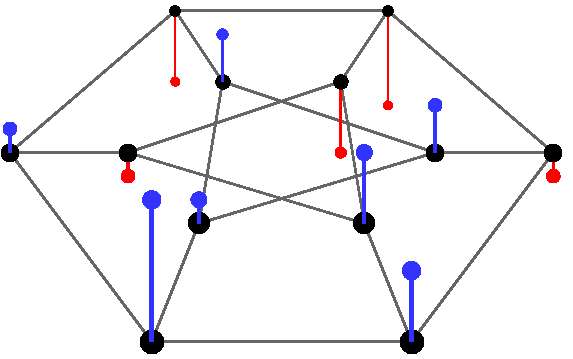
\includegraphics[width=0.25\linewidth]{Figures/signal_duher_graph_2.pdf}
	\caption{Example of signal defined over a graph. The height of the vertical bars indicate the value of the signal samples, which are indexed by the graph vertices. The graph edges capture similarity relations between samples. How could one define spectral analysis and processing techniques in such a signal domain?}
	\label{fig:duher}
\end{figure}

\subsection{The challenge of graph-like domains}

One of the reasons why GSP has been such a fertile field, allowing the birth of so many different problems and ideas, is that the definition of a signal over a graph leads to a series of obstacles even with fundamental concepts of signal processing. Let us use the simple but elucidating example given by Shuman \emph{et al.}~\cite{shuman2013emerging}, and consider the unit shift to the right of a discrete-time signal $ x[n] $, which is done in digital signal processing (DSP) by the simple variable substitution $ x[n-1] $. Good enough, but what does it mean to right-shift the signal in  Fig. \ref{fig:duher}, for example? Obviously the sense of right and left are meaningless for general graphs. On this problem, Shuman \emph{et al.} argue that a na\"ive choice would be to label the $ N $ graph vertices from $ v_0 $ to $ v_{N-1} $, so that the sample $ x[n] $ is assigned to vertex $ v_n $, for doing so would allow to define the shifted signal as the result of assigning $ x[n] $ to vertex $ v_{(n-1) \text{\,mod\,} N} $. Such an option, however, is not adequate, for its repeatability depends always on the way the vertices are labelled \cite{shuman2013emerging}. This example illustrates how a concept in DSP as simple as signal translation may deserve a cautious study in GSP.


\section{Principles and definitions}
\label{sec:II}
The field of graph signal processing draws basic concepts from the classical theories of digital signal processing and graph theory, aiming to provide a cohesive and useful framework to tackle the aforementioned challenges. In this section, some of the main definitions found in this field are presented.


\subsection{Graph theory: a brief terminology}

A graph is commonly defined as the ordered pair  $ (\mathcal{V},\mathcal{E}) $, in which the set $ \mathcal{V} $ contains the so called graph \emph{vertices} and the set of \emph{edges} $ \mathcal{E} $ is a subset of $ \mathcal{V}^2 $ \cite{feofiloff2011introduccao}.  We will usually indicate by $ |\mathcal{V}| = N $\footnote{The set operator $ |\cdot| $ means the cardinality, or amount of elements, of the set.} and $ |\mathcal{E}| = E $ the number of vertices and edges of a graph, respectively. For our purposes it is convenient to represent a graph as the structure $ \mathcal{G} = \{\mathcal{V}, \mathbf{A}\} $, endowed with the (weighted) adjacency matrix $ \mathbf{A} $ which captures the vertex-to-vertex relations: if $ A_{i,j} \neq 0$, then there is an edge of weight $ A_{i,j} $ from the vertex $ v_j $ to $ v_i $. It is denoted by $ d_i^- $ the \emph{indegree} of vertex $ v_i $, consisting of the sum of weights of all incoming edges to vertex $ v_i $. Likewise, the \emph{outdegree} $ d^+_i $ is the sum of weights of edges departing from $ v_i $.

A graph is called \emph{undirected} if and only if its adjacency matrix is symmetric, in which case it is defined the \emph{degree} of vertex $ v_i $ as $ d_i^- = d_i^+ = d_i $. In this case, a graph is said to be \emph{d-regular} whenever all graph vertices have degree $ d $\label{pag:regular}. If $ \mathbf{A} $ is asymmetric, however, the respective graph is \emph{directed} and its pictorial representation depicts the edges as arrows, to account for the unidirectional relation between adjacent vertices. Examples of directed and undirected graphs are shown in Fig. \ref{fig:example_graphs}.

\begin{figure}
	\centering
	\subfloat[]{
		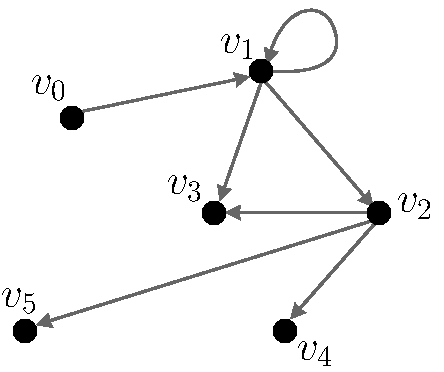
\includegraphics[width=0.25\linewidth]{Figures/example_graph_01_math.pdf}
	}~
	\subfloat[\label{fig:example_graphs_b}]{
		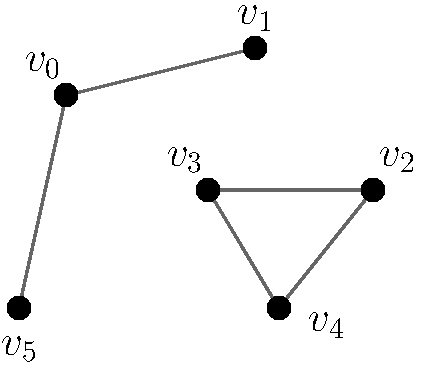
\includegraphics[width=0.25\linewidth]{Figures/example_graph_02_math.pdf}
	}
	\caption{Examples of (a) directed and (b) undirected graphs, defined over the same vertex set.}
	\label{fig:example_graphs}
\end{figure}

The adjacency matrix is the building block for one of the two main frameworks of GSP, what will be covered soon, but another matrix of great importance, mainly in the branch of GSP originated from spectral graph theory, is the Laplacian matrix
\begin{equation}
%\label{key}
\mathbf{L} = \mathbf{D} - \mathbf{A},
\end{equation}
with the \emph{degree matrix} $ \mathbf{D} $ being a diagonal matrix with the degree $ d_i $ as its $ i $-th entry. Depending on the context, $ \mathbf{D} $ may be taken as the indegree or outdegree matrix, although when the Laplacian matrix is used the graphs considered are more often undirected.

A \emph{path} is a set of distinct edges (with the same orientation, if the graph is directed) linking distinct vertices. A \emph{cycle} is a path with equal starting and end points, and if a graph has a cycle it is called \emph{cyclic} (\emph{acyclic}, otherwise). If the cycle has only one edge, it is called a \emph{loop}. One refers to \emph{multiple edges} whenever a single pair of vertices is connected by two or more edges. An undirected graph is called \emph{simple} if it has no loops or multiple edges.

A graph is said to be \emph{complete} if any two of its vertices are adjacent. Graph signal processing over such graphs may be extremely cumbersome, for the computational complexity of many of its techniques depends heavily on the number of graph edges. For most applications, it is desirable to have a small number of edges while keeping the graph \emph{connected}, i.~e. for any pair of vertices there exists a set of distinct edges (with the same orientation, if directed) connecting them without making a cycle.

A graph is said to be \emph{unweighted} if all its edges have unit weight. A \emph{subgraph} of $ \mathcal{G} $ is a graph $ \mathcal{G}' = (\mathcal{V}', \mathbf{A}')$ with edge set $ \mathcal{E}' $, in which $ \mathcal{V}' \subset \mathcal{V} $ and $ \mathcal{E}' \subset \mathcal{E} $. A \emph{connected component} of $ \mathcal{G} $ is a connected subgraph $ \mathcal{G}' = (\mathcal{V}', \mathbf{A}')$ in which any vertex in $ \mathcal{V}' $ is linked exclusively to another vertex also in $ \mathcal{V}' $. This is illustrated by Fig. \ref{fig:example_graphs_b}, in which the graph has two connected components.

\begin{figure}
	\centering
	\subfloat[\label{fig:k_hop_neighborhood_01}]{
		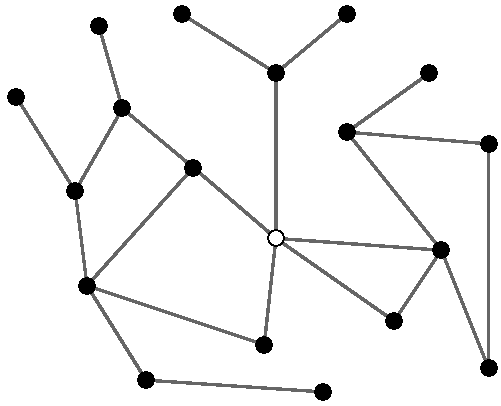
\includegraphics[width=0.25\linewidth]{Figures/k_hop_neighborhood_01.pdf}
	}~
	%	\qquad
	\subfloat[\label{fig:k_hop_neighborhood_02}]{
		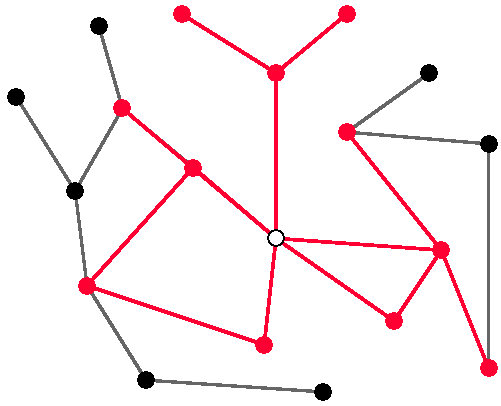
\includegraphics[width=0.25\linewidth]{Figures/k_hop_neighborhood_02.pdf}
	}
	%\hspace{0.2cm}%
	\caption{(a) A graph and (b) the set of vertices $ \mathcal{N}(i,2) $ shown in red, with $ v_i $ being depicted in white. The edges linking $ v_i $ to the elements in $ \mathcal{N}(i,2) $ are also highlighted in red.}%
	\label{fig:k_hop_neighborhood}%
\end{figure}

The \emph{neighbourhood} of a vertex $ v_i $ is the set $ \mathcal{N}_i $ of all vertices adjacent to $ v_i $. Sometimes it is useful as well to denote by $ \mathcal{N}(i,K) $ the set of vertices connected to $ v_i $ through a path of length $ K $ or less. This notion is represented in Fig. \ref{fig:k_hop_neighborhood}.

The reader is encouraged to refer to this section whenever necessary. For a broader glossary with a solid introduction to graph theory, the authors recommend \cite{bondy2008graph,chung1997spectral}.


\subsection{Defining a graph signal}

A signal $ \mathbf{s} $ defined over $ \mathcal{G} = \{\mathcal{V}, \mathbf{A}\} $, with $ |\mathcal{V}| = N $, is a discrete-domain function mapping the graph vertex set to a scalar set, usually the complex or real numbers,
\begin{equation}
	%\label{key}
	s: \ \mathcal{V} \rightarrow \mathbb{C} \ | \ s(v_i) = s_i,
\end{equation}
so that $ \mathbf{s} $ can be seen as a vector in $ \mathbb{C}^N $ \emph{indexed by the vertices of} $ \mathcal{G} $. Once the vertices $ \mathcal{V} = \{v_1, \dots, v_N\}$ are clearly labelled, it is not ambiguous to represent the signal as the column vector $ \mathbf{s} = (s_0 \ s_1 \ \dots \ s_{N-1})^T$, $ s_i \in \mathbb{C} $, $ 0 \leq i \leq N-1 $.

\begin{figure*}
	\centering
	\subfloat[\label{figa_graphs}]{
		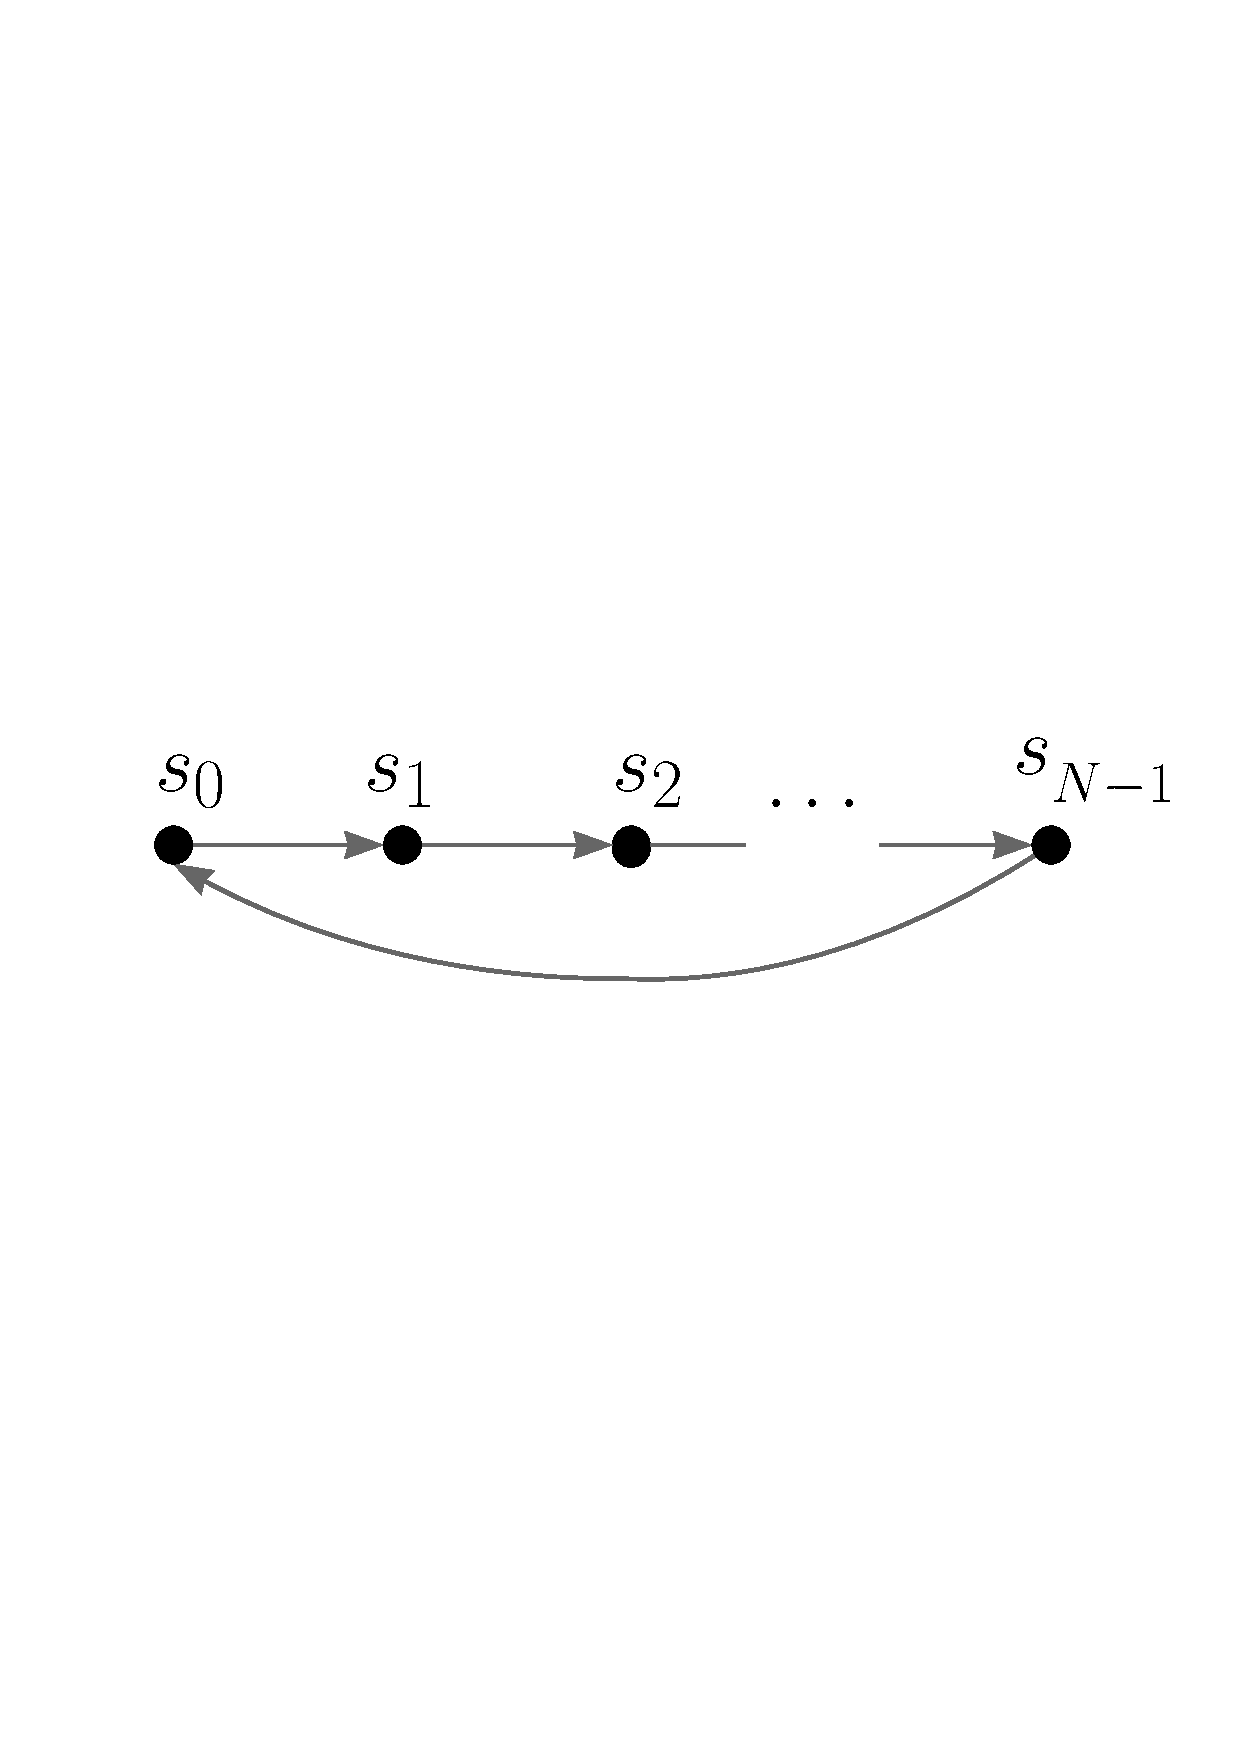
\includegraphics[width=0.25\linewidth]{Figures/signal_ring_graph_white_border.pdf}
	}
	%		\hspace{0.2cm}%
	%	\qquad
	%	\subfloat[t][\label{figb_graphs}]{
	%		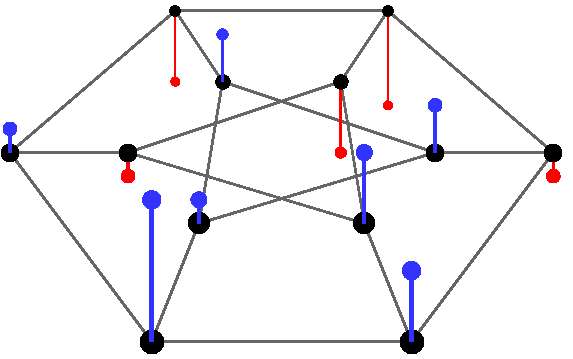
\includegraphics[width=0.25\linewidth]{Figures/signal_duher_graph_2.pdf}
	%	}
	\subfloat[\label{figb_graphs}]{
		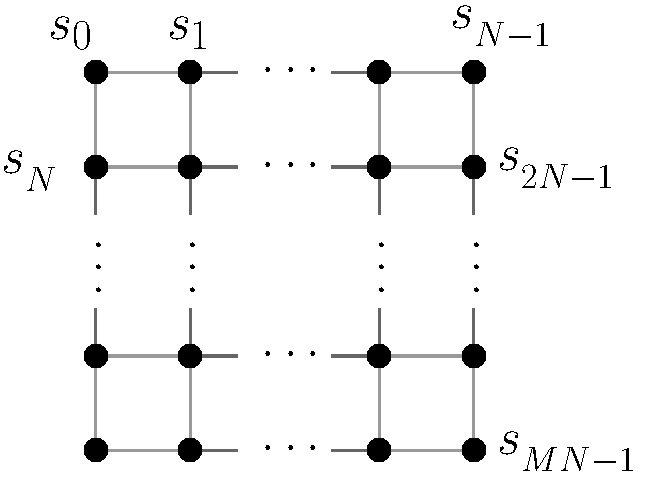
\includegraphics[width=0.25\linewidth]{Figures/image_graph.pdf}
	}%
	\subfloat[\label{figd_graphs}]{
		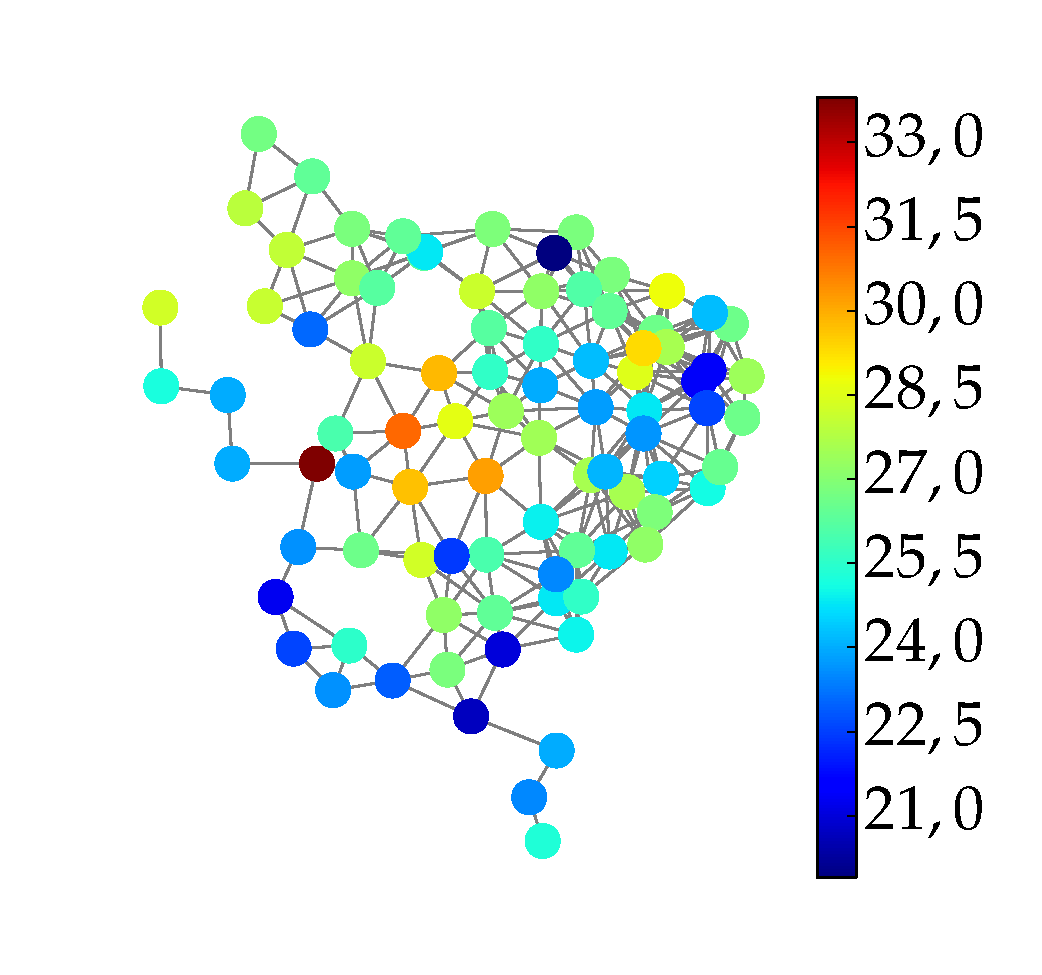
\includegraphics[width=0.3\linewidth]{Figures/temp_NE_stretched.pdf} }%
	\caption{Examples of depictions of graph signals over (a) a directed ring graph, 
		%	(b) um grafo de D\"{u}her n\~ao-direcionado,
		(b) an undirected regular grid graph and (c) a graph of cities from the Brazilian Northeastern region, over which was defined a signal of temperature measurements from February 1\textsuperscript{st} of 2012, retrieved from the
		\emph{Banco de Dados Meteorol\'ogicos para Ensino e Pesquisa} (BDMEP, freely translated as Meteorological Database for Teaching and Research), available at: \url{http://www.inmet.gov.br/portal/index.php?r=bdmep/bdmep}.}%
	\label{fig:graphs}%
	\vspace{-0.2cm}
\end{figure*}

%\footnote{Fonte: Banco de Dados Meteorol\'ogicos para Ensino e Pesquisa (BDMEP) do Instituto Nacional de Meteorologia. Acesso gratuito ap\'os cadastro, dispon\'ivel em: \url{http://www.inmet.gov.br/portal/index.php?r=bdmep/bdmep}.}

Fig. \ref{fig:graphs} provides examples of graph signal representations, in which the vertex labelling is omitted for the sake of simplicity, as it will be assumed that the signal sample $ s_i $ is assigned to vertex $ v_i $. The signal values are indicated in two manners: either by writing down its numerical value next to the respective vertex, or by using a pseudocolor scale, the latter of which is the scheme adopted throughout this paper.

%Por ora, o leitor pode ter-se indagado sobre a pr\'opria \emph{constru\c c\~ao} do grafo para o caso de sinais reais, como aquele obtido de medi\c c\~oes de temperatura na Fig. \ref{figd_graphs}, o que de fato n\~ao \'e uma quest\~ao trivial e ser\'a abordada na subse\c c\~ao a seguir.

It is crucial to stress a certain graph which links GSP to the classical Discrete Signal Processing (DSP) theory: the directed ring graph, shown in Fig. \ref{figa_graphs}, which models the finite-length discrete-time domain. Its directed edges model the causality of time domain, whereas the feedback edge accounts for the boundary condition of periodicity imposed by the DFT analysis. Other signals that arise in practical applications have the respective graphs easily identified: the rectangular lattice in Fig. \ref{figb_graphs}, for example, models the digital image domain \cite{sandryhaila2012nearest}, and Fig. \ref{figd_graphs} shows an example of signal defined over a mesh network of sensors, with the edges weighted using the inverse of the euclidian distance, which arises in many scenarios such as IoT applications.

\begin{figure*}
	\centering
	\begin{minipage}[c]{0.24\linewidth}
		\subfloat[\label{fig:diff_struct_a}]{
			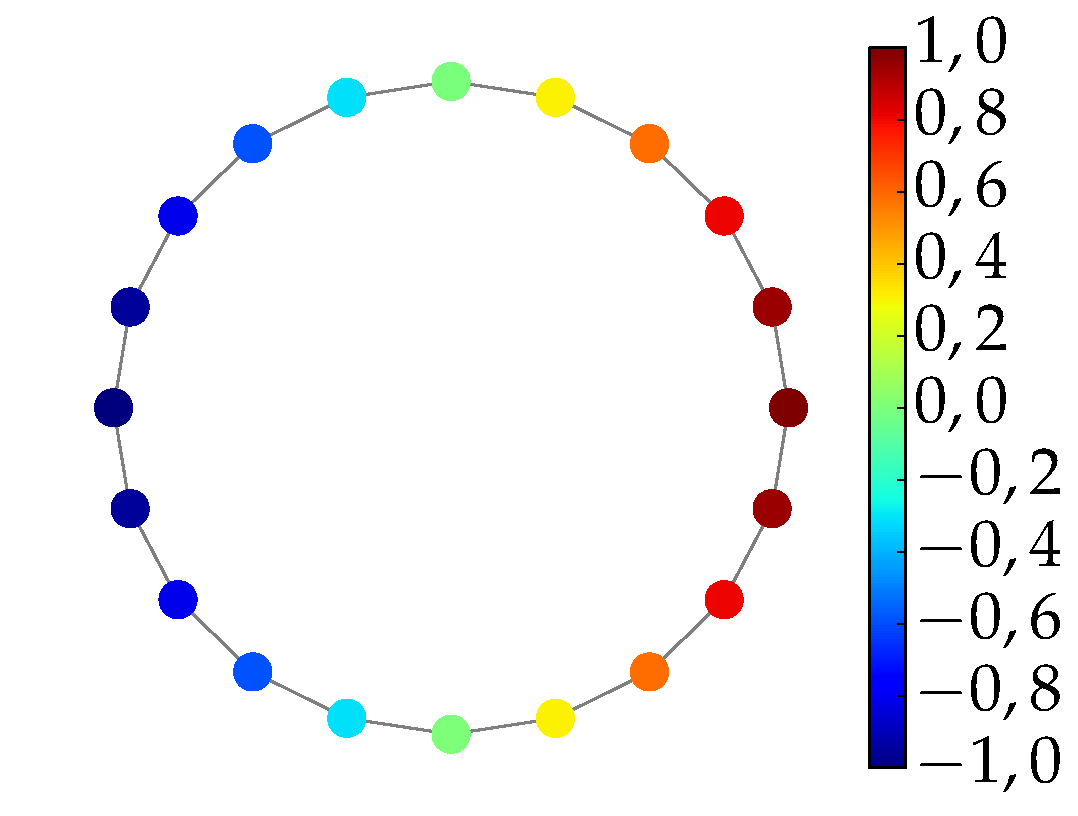
\includegraphics[width=\linewidth]{Figures/ring_different_structure_01.pdf}
		}
	\end{minipage} %
	\begin{minipage}[c]{0.24\linewidth}
		\subfloat[\label{fig:diff_struct_c}]{
			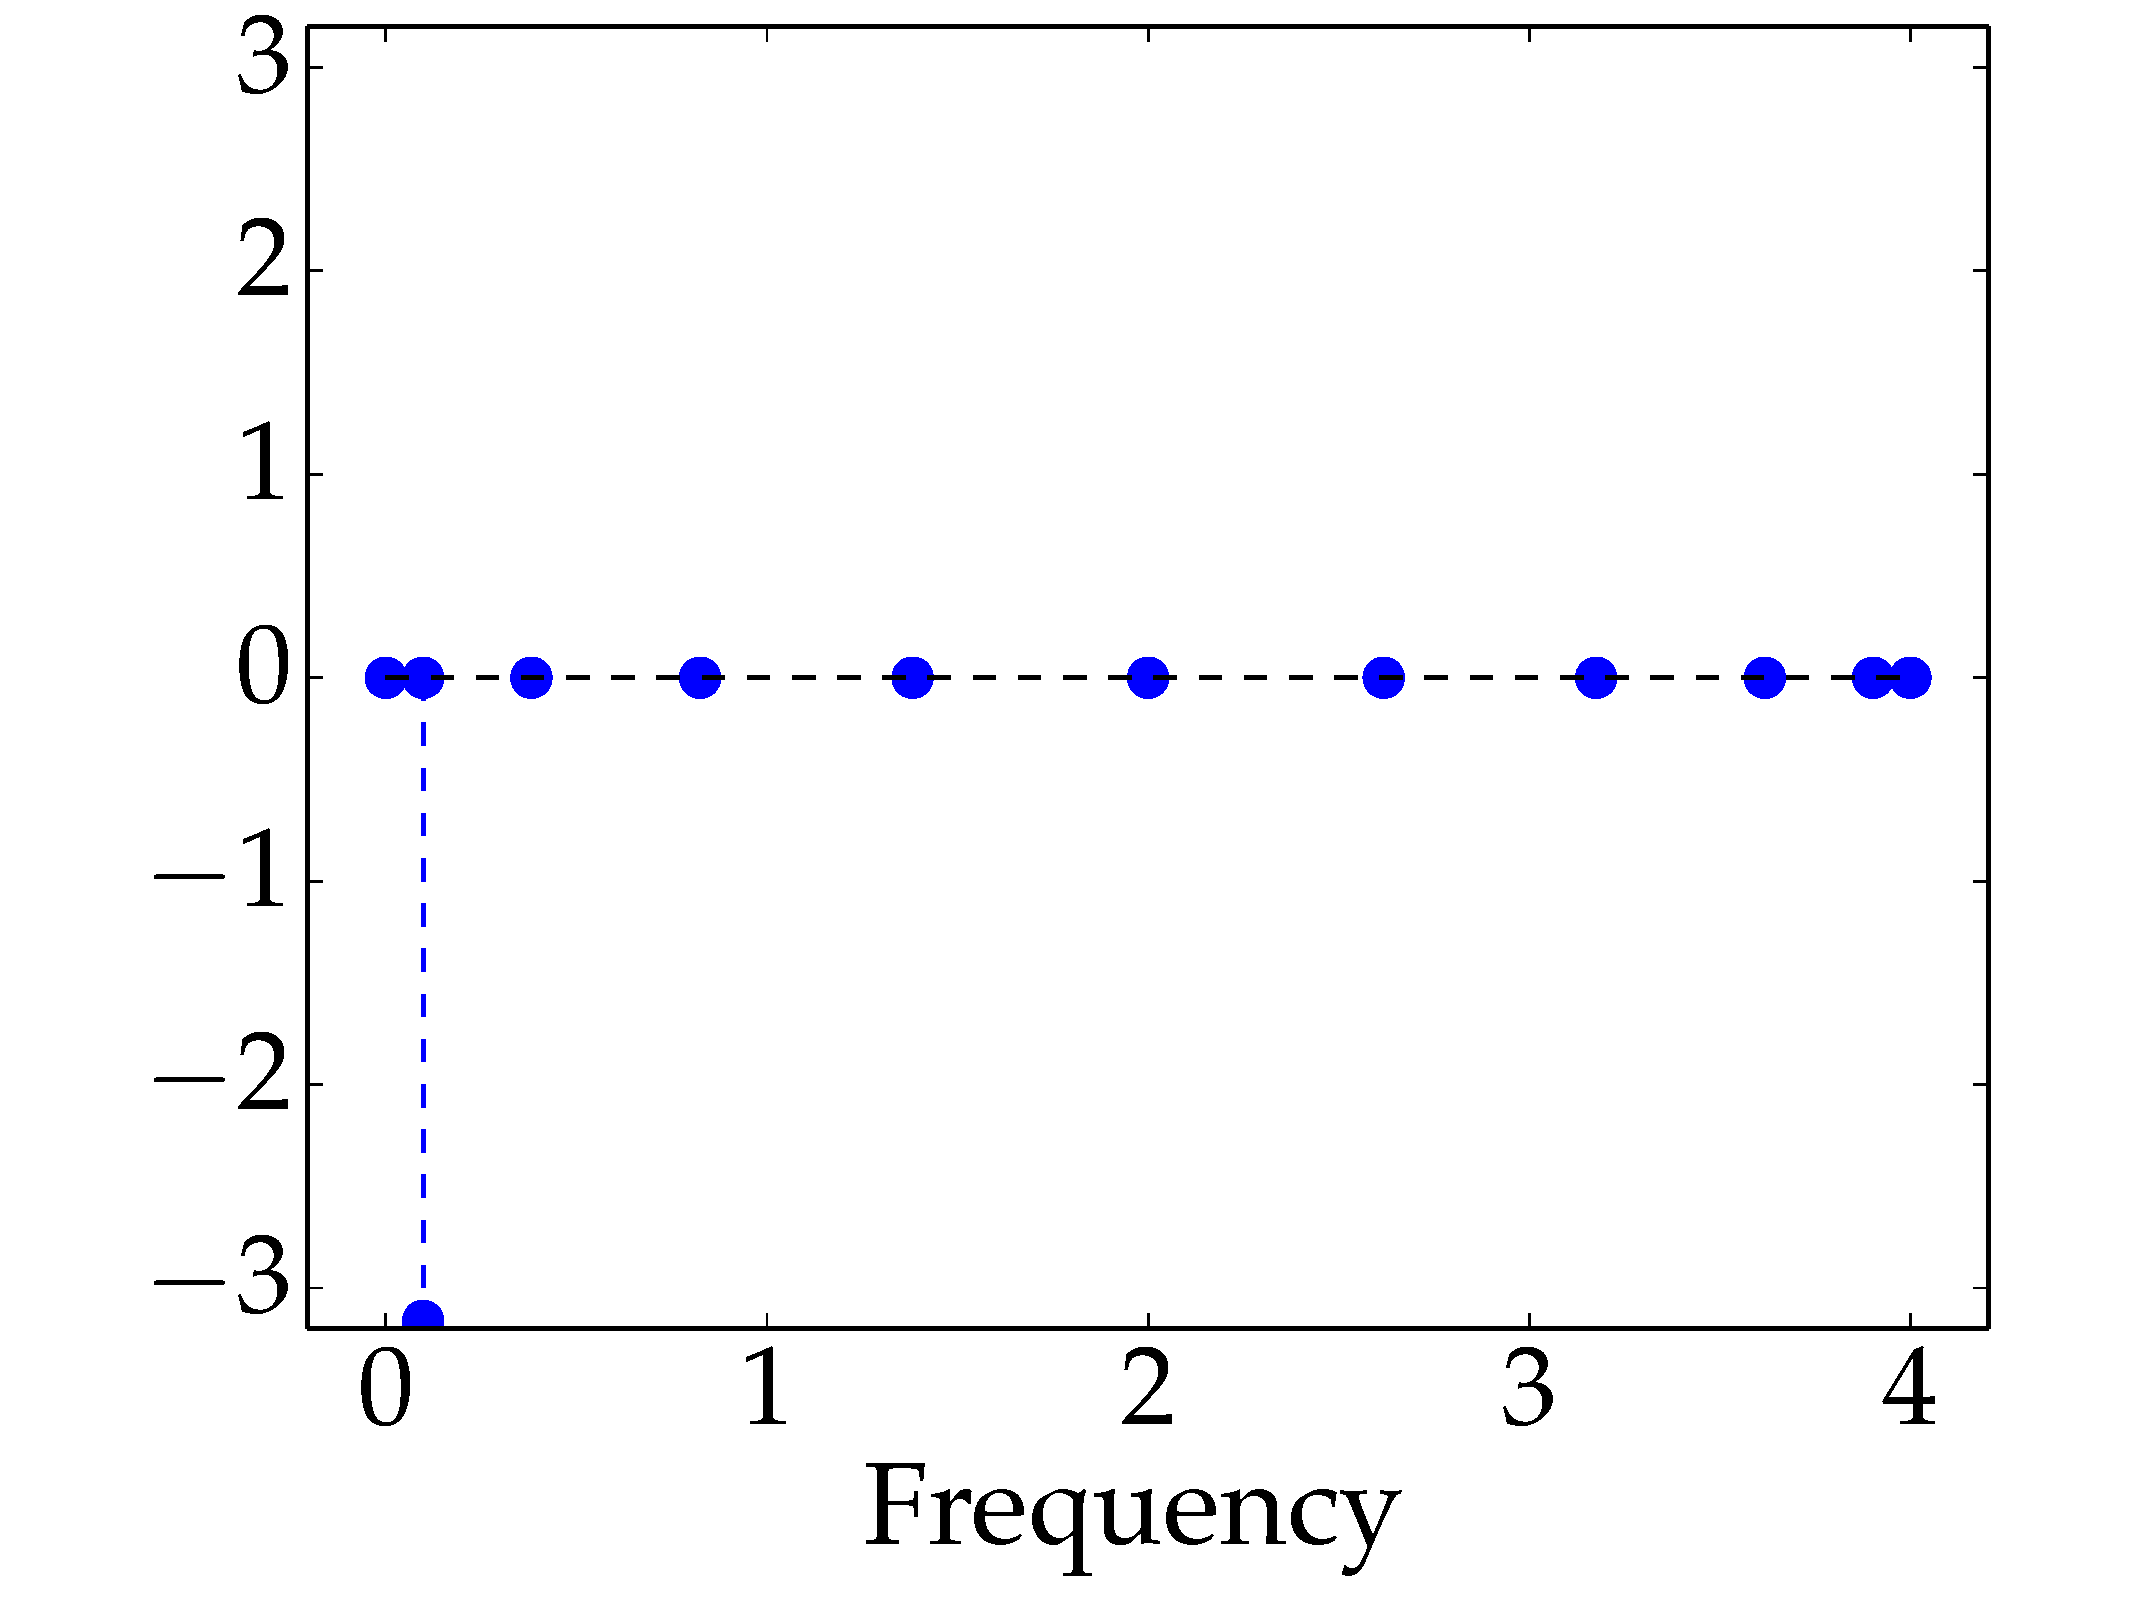
\includegraphics[width=\linewidth]{Figures/ring_different_structure_01_spectrum_EN.pdf}
		}
	\end{minipage}%
	\begin{minipage}[c]{0.24\linewidth}
		\subfloat[\label{fig:diff_struct_b}]{
			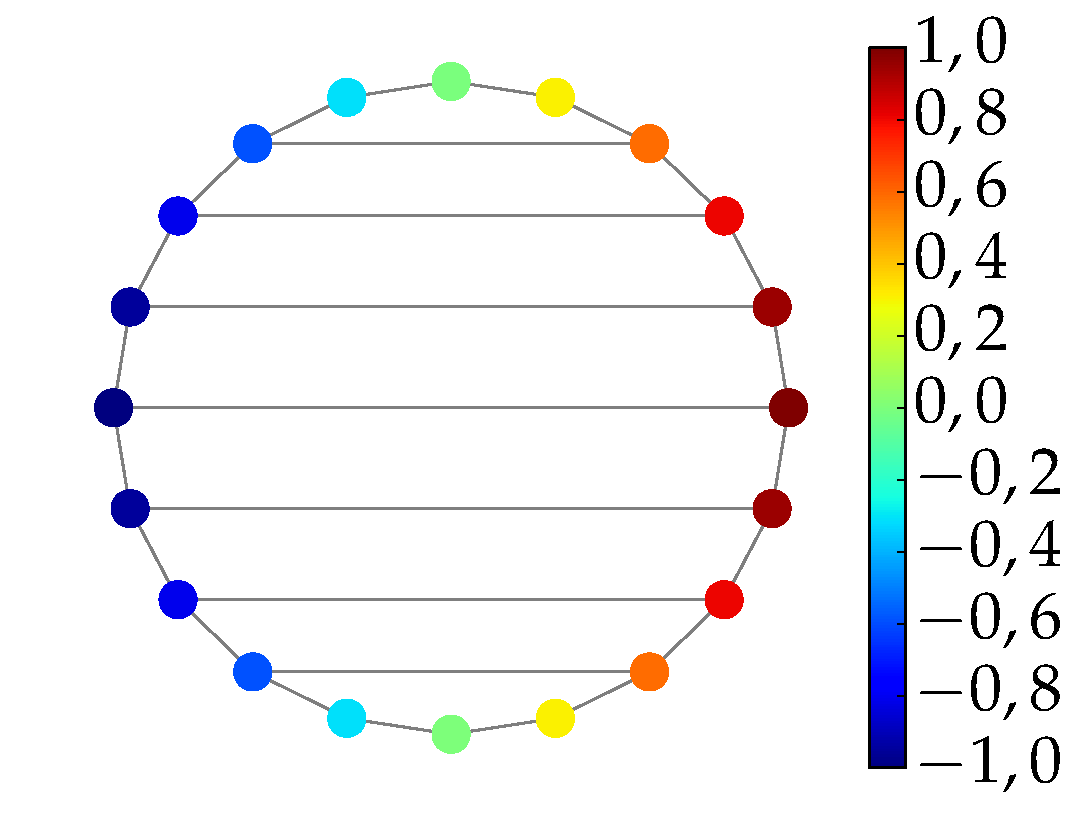
\includegraphics[width=\linewidth]{Figures/ring_different_structure_02.pdf}
		}~
	\end{minipage}%
	\begin{minipage}[c]{0.25\linewidth}
		\subfloat[\label{fig:diff_struct_d}]{
			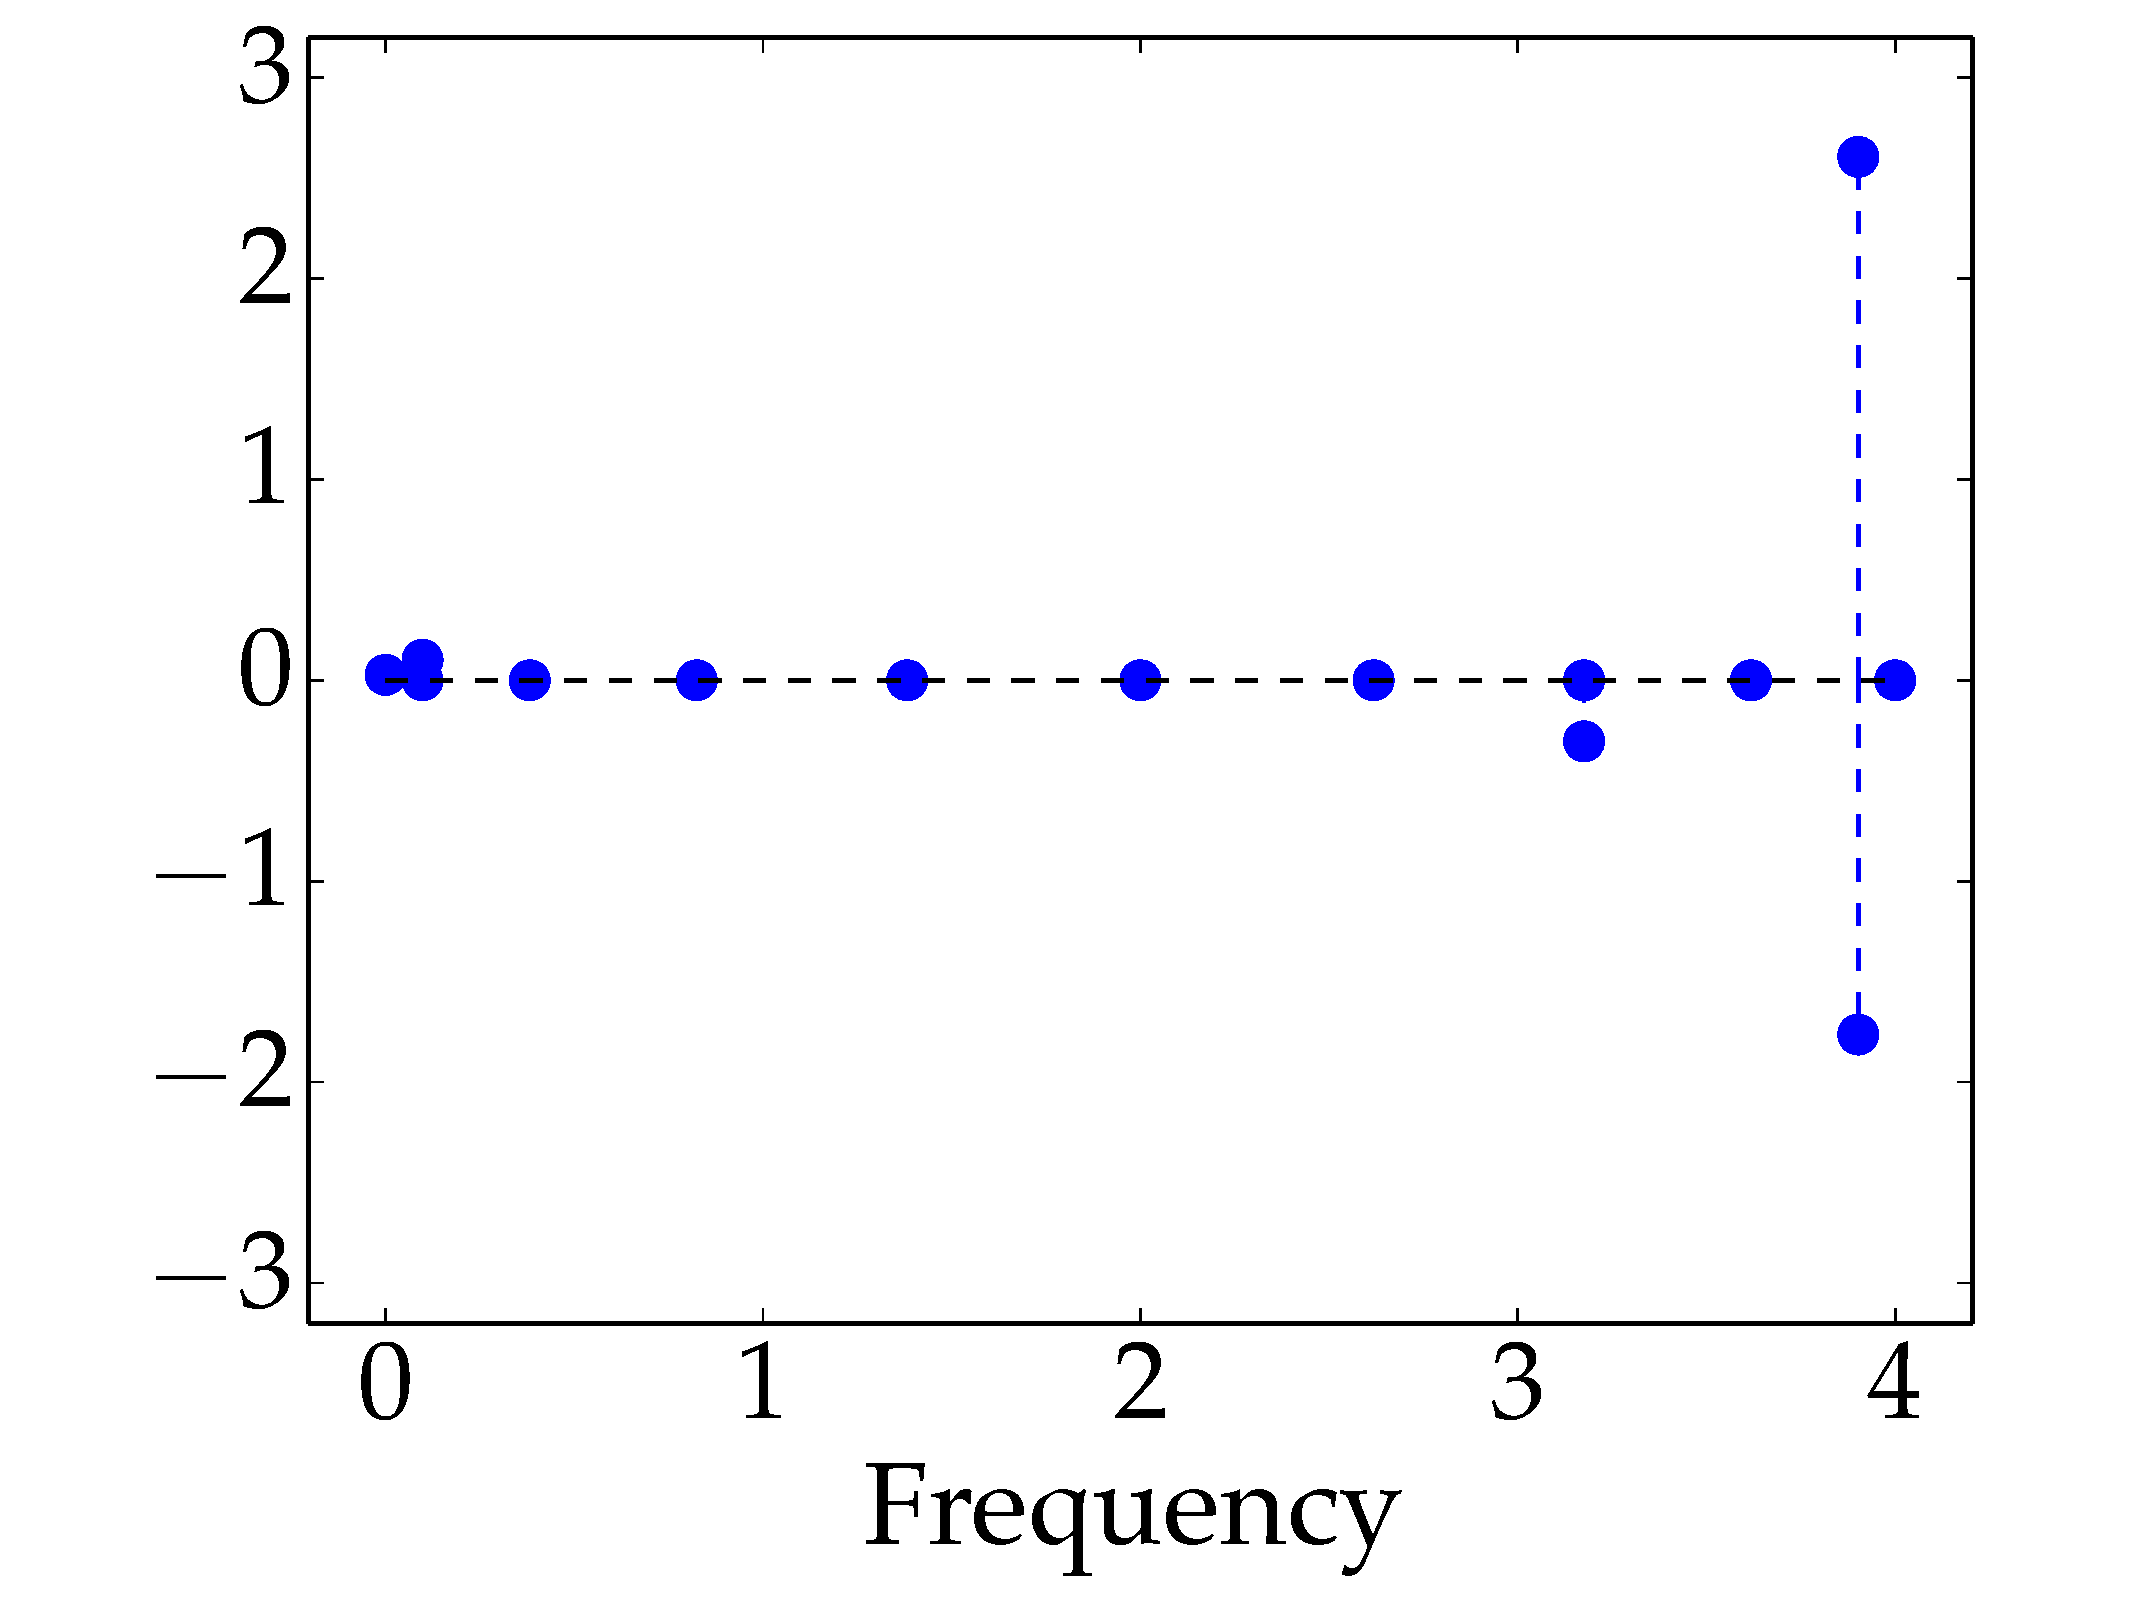
\includegraphics[width=\linewidth]{Figures/ring_different_structure_02_spectrum_EN.pdf}
		}
	\end{minipage}%
	\caption{The same signal was defined over similar graphs, one of them being (a) the undirected ring graph. In (b) and (d) are depicted the Fourier spectra according to GSP\textsubscript{L} (as defined in Subsection \ref{subsec:GFT_L}) of the signals in (a) and (c), respectively.}%
	\label{fig:diff_struct}%
	\vspace{-0.2cm}
\end{figure*}

The spectral characteristics of a signal depend heavily on the domain over which it is defined, but one does not need to acknowledge this in the context of DSP, for in this case the domains are always regular and uniform\footnote{One could argue that, in the theory of \emph{nonuniform sampling}, the signal is defined over an irregular domain, since the samples may be randomly spaced. Even in this case, however, the classical techniques still aim to \emph{recover} the signal so as to represent it in its usual -- and \emph{uniform} -- domain.
%Even when considering \emph{nonuniform sampling}, theory in which one could argue the signal is defined over an irregular domain, since the samples may be randomly spaced, the classical techniques still aim to \emph{recover} the signal and represent it in a domain typically uniform.
}.
From the classical theory, the common understanding states that a signal has mostly low frequencies if adjacent samples have similar values, and high frequencies otherwise. When dealing with signals defined over graphs, it is clear that the adjacency relations depend on the graph topology, and therefore one may foresee that \emph{the same signal may present different spectra when defined over different graphs}. This intuition is visually confirmed (and will soon be mathematically proved) in Fig. \ref{fig:diff_struct}, which depicts a signal and its spectra when two different graphs are taken as a domain. The reader may notice that, in Fig. \ref{fig:diff_struct_b}, the samples with highest values are adjacent to the ones with small values, what causes bigger frequency components in this signal than in the one defined over the undirected ring graph in Fig. \ref{fig:diff_struct_a}.

\subsection{Graph inference}
\label{subsec:inferindo}

Some contexts in which GSP is to be applied, to perform whatever signal processing technique is necessary, do not provide clear information on \emph{how the underlying graph is structured}. For example, let us suppose the temperature data (or any other data in fact) of some Brazilian Northeastern cities will be treated using GSP. How is one supposed to weight the graph edges, and before this, how does one decide which vertices to connect? Is the graph shown in Fig. \ref{figd_graphs} the only option? Clearly not. Although generally the problem of graph inference is complex, this type of geography-based graph has an adequate method topology estimation.

The general ideia is that, if there is a clear metric to evaluate the \emph{expected} similarity between samples as a function of the available information regarding the respective vertices, then this metric may be used as the edge weight and a threshold is set so that any weight below this value causes the respective edge to be eliminated. In the case of vertices which have geodesic positions, the euclidian distance may be used as the metric because vertices that are closer together are \emph{expected} to have similar signal samples, and therefore the adjacency matrix of the underlying graph may have entries given by
\begin{equation}
\label{eq:weights}
A_{ij} =
\begin{cases}
\displaystyle
\exp \left(- \frac{\text{dist}^2(v_i, v_j)}{2 \theta^2}\right)& \text{ if } \text{dist}(v_i, v_j) < T \\ 
0 & \text{ otherwise},
\end{cases}
\end{equation}
as used in \cite{shuman2013emerging}. The choice of the parameters $ T $\footnote{$ T $ indicates a distance threshold above which we set the edge weight to zero, effectively leaving the vertices unlinked. This means that the distance between them is assumed to be too high for any significant interdependence to exist.} and $ \theta $ (standard deviation of the distribution), and of how to use the metric (in this case, inside a Gaussian distribution), are dictated by the application and by the analyst experience. 

However, if there is an isolated vertex, far from the others, the use of (\ref{eq:weights}) may lead to a compromise between keeping the graph connected and obtaining a sparse adjacency matrix, since imposing connectivity to the graph in this case implies increasing $ T $, and therefore having many edges. To deal with this problem and still have a good representation of the underlying graph, one alternative is to connect a vertex to its $ K $ closest neighbours (setting $ K $ to an appropriate value, according to the context) and weight the edges using the Gaussian distribution in (\ref{eq:weights}).

As previously discussed, these methods require an adequate metric to evaluate the expected similarity between samples in the graph vertex, but given the diverse areas in which graph signals may arise, estimating the topology of the  underlying graph constitutes a challenge of its own \cite{mei2016signal,Sardellitti2016}.

\section{Formulating GSP based on the graph adjacency matrix}
\label{sec:DSPG}

In 2008, P\"uschel and Moura published their \emph{algebraic signal processing} (ASP) theory \cite{puschel2008time,puschel2008space}, which expands DSP by moving to an algebraic point of view: each signal processing theory is studied as a triple $ (\mathscr{A}, \mathscr{M}, \Phi) $ consisting of an algebra $ \mathscr{A} $ (a vector space endowed with multiplication between vectors), an $ \mathscr{A} $-module $ \mathscr{M} $ (a vector space over the same base field as $ \mathscr{A} $ which admits left-multiplication by elements of $ \mathscr{A} $) and a linear transformation $ \Phi $. $ \mathscr{A} $ is called the filter space, $ \mathscr{M} $ is the signal space and $ \Phi $ is the Fourier transform (homomorphism over $ \mathscr{M} $) associated to the structure.

When these authors drew inspiration from ASP to develop their GSP theory, the starting point was necessarily to find (better, to define) the unit shift operator of graph signals, the reason being that such an operator in ASP is the building block of the algebra $ \mathscr{A} $ (as, for example, the unit delay $ z^{-1} $ is the building block for filters of discrete-time and finite-length signals $ \mathscr{A}  = \{ \sum_{\ell=0}^{N-1} h_\ell z^{-\ell} | h_\ell \in \mathbb{C} \}$). To do so, the shift of discrete-time signals, defined over directed ring graphs, was investigated.

By inspection of the \emph{adjacency matrix} of the directed ring graph,
\begin{equation}\label{eq:C}
\mathbf{C} =
\begin{bmatrix}
&  &  &   1\\ 
1 &  &   & \\ 
&   \ddots &  & \\ 
&  &   1 & 
\end{bmatrix},
\end{equation}
it was noticed that the unit (circular) shift of discrete-time signals is precisely the left-multiplication by $ \mathbf{C} $, for given a discrete-time signal $ \mathbf{x} = (x_0 \ x_1 \ \dots \ x_{N-1})^T $,
\begin{equation}\label{eq:unit_shift}
\mathbf{C}\mathbf{x} =
\begin{bmatrix}
&  &  &   1\\ 
1 &  &   & \\ 
&   \ddots &  & \\ 
&  &   1 & 
\end{bmatrix}
\begin{bmatrix}
x_0 \\ x_1 \\ \vdots \\ x_{N-1}
\end{bmatrix} =
\begin{bmatrix}
x_{N-1} \\ x_0 \\ \vdots \\ x_{N-2}
\end{bmatrix} \overset{\Delta}{=} \mathbf{x}^{\langle 1 \rangle},
\end{equation}
and the generalization followed: \emph{the graph unit shift was defined as the left-multiplication by the graph adjacency matrix}. This is the reason why in this paper the branch of GSP developed by Sandryhaila, Moura and their peers is referred to as GSP\textsubscript{A}, to indicate the fundamental role of the matrix $ \mathbf{A} $.

In other words, for a signal $ \mathbf{x} $ defined over the graph $ \mathcal{G} = \{\mathcal{V}, \mathbf{A}\} $, the adjacency matrix $ \mathbf{A} $ acts as a \emph{filter} which ``delays'' (i.~e. translates) $ \mathbf{x} $ by one unit, producing the delayed version represented hereinafter by $ \mathbf{x}^{\langle 1 \rangle} = \mathbf{A} \mathbf{x}$.

\subsection{Graph filters}
\label{subsec:filtros}

Seeing the adjacency matrix as a filter suggested the general definition of \emph{graph filter} as any matrix $ \mathbf{H} \in \mathbb{C}^{N \times N} $ \cite{sandryhaila2013filters}, which preserves the necessary property that the output of a filter (i.~e. the matrix-vector product) is a signal (i.~e. a vector). Such a definition implies that \emph{linearity} is always valid for graph filters, since the distributivity of matrix multiplication with respect to matrix addition guarantees that
\begin{equation}
%\label{key}
\mathbf{H} (\alpha_1 \mathbf{x}_1 + \alpha_2 \mathbf{x}_2) =  \alpha_1 \mathbf{H} \mathbf{x}_1 + \alpha_2 \mathbf{H}  \mathbf{x}_2.
\end{equation}

The next desirable property would be \emph{shift invariance}, analogous to the classical time invariance of DSP, and this means that filtering and shifting should commute. In other words, for a graph filter $ \mathbf{H} $ to be \emph{linear and shift invariant} (LSI) it is required that $ \mathbf{A} \mathbf{H} \mathbf{x} = \mathbf{H} \mathbf{A} \mathbf{x} \ \forall \mathbf{x}$, and therefore $ \mathbf{A} \mathbf{H} = \mathbf{H} \mathbf{A}$. Sandryhaila and Moura have shown \cite{sandryhaila2013discrete,sandryhaila2014big} that LSI filters can be represented as polynomials $ h(\cdot) $ evaluated over $ \mathbf{A} $,
\begin{equation}
\label{eq:filter_poly}
h(\mathbf{A}) = \sum_{\ell=0}^{L-1} h_\ell \mathbf{A}^\ell,
\end{equation}
with $ L $ smaller than or equal to the degree of the minimal polynomial of $ \mathbf{A} $, i.~e. filters LSI are finite power series on the shift operator, exactly as happens in DSP, in which LTI filters have polynomial representations on $ z^{-1} $.

\subsection{Graph Fourier transform}

The topic of spectral analysis is key in signal processing, and the authors of GSP\textsubscript{A} would certainly want to spend time reflecting upon how this would fit into their theory. The starting point was to look to the classical Fourier transform as the signal decomposition into a basis of eigenfunctions of the LTI filtering \cite{oppenheim1997signals}, as is indeed the basis of complex time exponentials. Then, the \emph{graph Fourier transform} (GFT) could be defined as the decomposition into a basis of eigenvectors of LSI filtering.

Let us take the graph $ \mathcal{G} = \{\mathcal{V}, \mathbf{A}\} $, $ |\mathcal{V}| =N $. If $ \mathbf{A} $ is diagonalizable\footnote{If not, the reasoning may be replicated using the Jordan decomposition of $ \mathbf{A} $.}, then one may write
\begin{equation}\label{eq:gft_01}
\mathbf{A} = \mathbf{V} \mathbf{\Lambda} \mathbf{V}^{-1},
\end{equation}
in which $ \mathbf{V} $ contains the $ N $ eigenvectors of $ \mathbf{A} $ in its columns,
\begin{equation}\label{eq:gft_02}
\mathbf{V} = (\mathbf{v}_0 \ \mathbf{v}_1 \ \dots\ \mathbf{v}_{N-1}).
\end{equation}

Since LSI filters are polynomials in $ \mathbf{A} $, and since a matrix and its powers share the same set of eigenvectors, the columns of $ \mathbf{V} $ form a basis of vectors invariant to LSI filtering. Besides, given that the subspaces generated by the linearly independent eigenvectors of a same eigenvalue of $ \mathbf{A} $ are irreducible, have null intersection and the dimensions of all subspaces add to $ N $ \cite{sandryhaila2013gft}, $ \mathbf{V} $ provides a basis which is invariant to LSI filtering for the space of signals defined over $ \mathcal{G} $.

Therefore, a signal $ \mathbf{x} $ may be decomposed into its components with respect to $ \mathbf{V} $ as
\begin{align}\label{eq:GFT_inv}
\mathbf{x} &= \widehat{x}_0 \mathbf{v}_0 + \dots + \widehat{x}_{N-1} \mathbf{v}_{N-1} \notag \\
&= \mathbf{V} (\widehat{x}_0 \ \widehat{x}_1 \ \dots \ \widehat{x}_{N-1})^T \notag \\
&= \mathbf{V} \widehat{\mathbf{x}},
\end{align}
and this is the synthesis equation of the GFT according to GSP\textsubscript{A}. The analysis equation follows,
\begin{equation}\label{eq:GFT_fwd}
\widehat{\mathbf{x}} = \mathbf{V}^{-1} \mathbf{x}.
\end{equation}

It has been emphasized that the directed ring graph is the link between GSP and DSP, because it models the discrete-time domain. This provides a way of checking how consistent with the classical theory are the proposed GSP tools. When investigating how the GFT would act upon discrete-time signals, one should first diagonalize the adjacency matrix $ \mathbf{C} $ of the directed ring graph, given by (\ref{eq:C}). Since it is circulant, it is known to be diagonalized by the DFT matrix $ \mathbf{F} $, with entries $ F_{n,k} = \exp \left( -j\frac{2 \pi}{N} nk \right) $, which contains in its \emph{rows} the DFT eigenvectors. The calculation of the characteristic polynomial of $ \mathbf{C} $,
\begin{equation}
%\label{key}
p_{\mathbf{C}}(\lambda) = \text{det} (\lambda \mathbf{I} - \mathbf{C}) =
\begin{vmatrix}
\lambda &  &  &   -1\\ 
-1 & \lambda &   & \\ 
&   \ddots & \ddots & \\ 
&  &   -1 & \lambda
\end{vmatrix}
=\lambda^N - 1,
\end{equation}
shows that its eigenvalues are the $ N $ complex roots of unity. Setting these eigenvalues as the entries of a diagonal matrix $ \mathbf{\Lambda}_{\mathbf{C}} $, the eigendecomposition of $ \mathbf{C} $ may be written as
\begin{equation}\label{eq:diag_C}
\mathbf{C} = \mathbf{F}^{-1} \mathbf{\Lambda}_{\mathbf{C}} \mathbf{F},
\end{equation}
and one can see that, in the case of directed ring graphs, the GFT and the DFT matrices \emph{coincide}, since $ \mathbf{V}^{-1} = \mathbf{F} $. This equivalence indicates a desirable consistency with the classical theory.

 \subsection{The frequency domain}

The GFT in the sense of GSP\textsubscript{A} naturally suggests the interpretation of the adjacency matrix eigenvectors $ \mathbf{v}_i $ as ``frequency components'' associated to the ``graph frequencies'' given by the eigenvalues $ \lambda_i $, exactly as the Fourier component $ e^{-j \Omega t} $, in the continuous time domain $ t $, is associated to the frequency $ \Omega $. This subsection aims to provide the mathematical justification used by Sandryhaila and Moura \cite{sandryhaila2014frequency} to support this understanding, along with some of our own comments.

%\begin{figure}
%	\centering
%	\subfloat[\label{fig:diff_struct_a_GSPA}]{
%		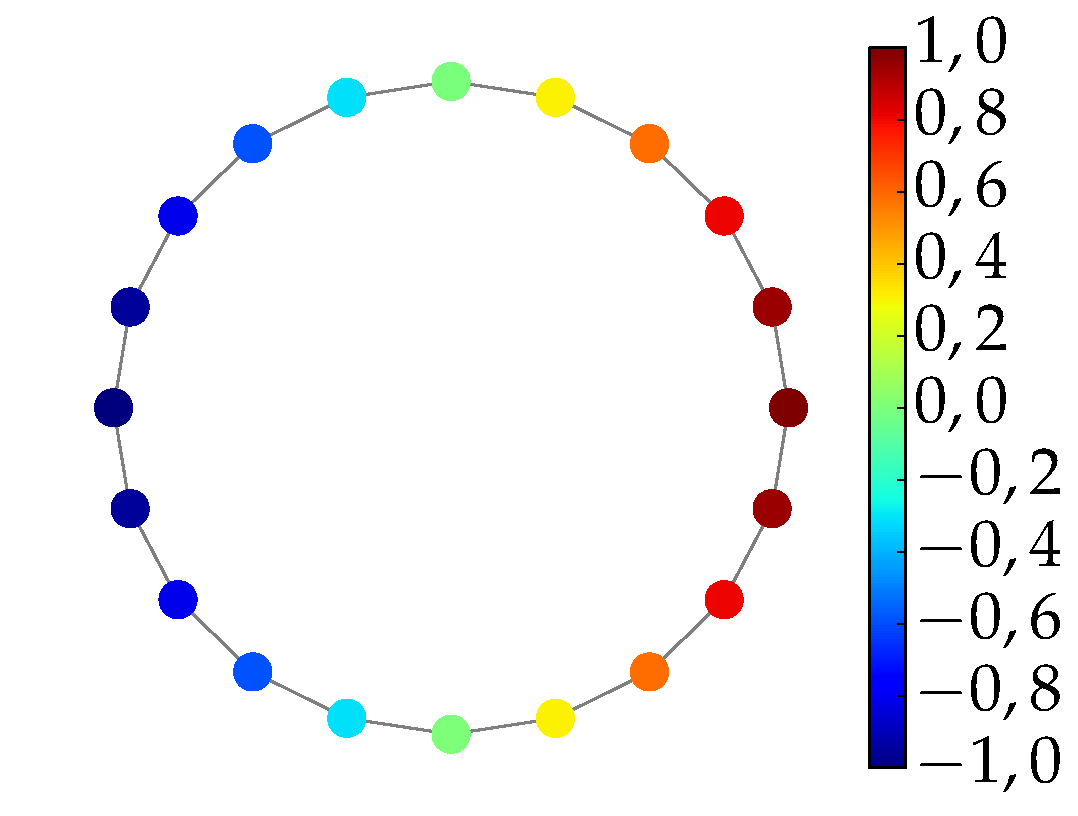
\includegraphics[width=0.35\linewidth]{Figures/ring_different_structure_01_GSPA.pdf}
%	}
%	\subfloat[\label{fig:diff_struct_b_GSPA}]{
%		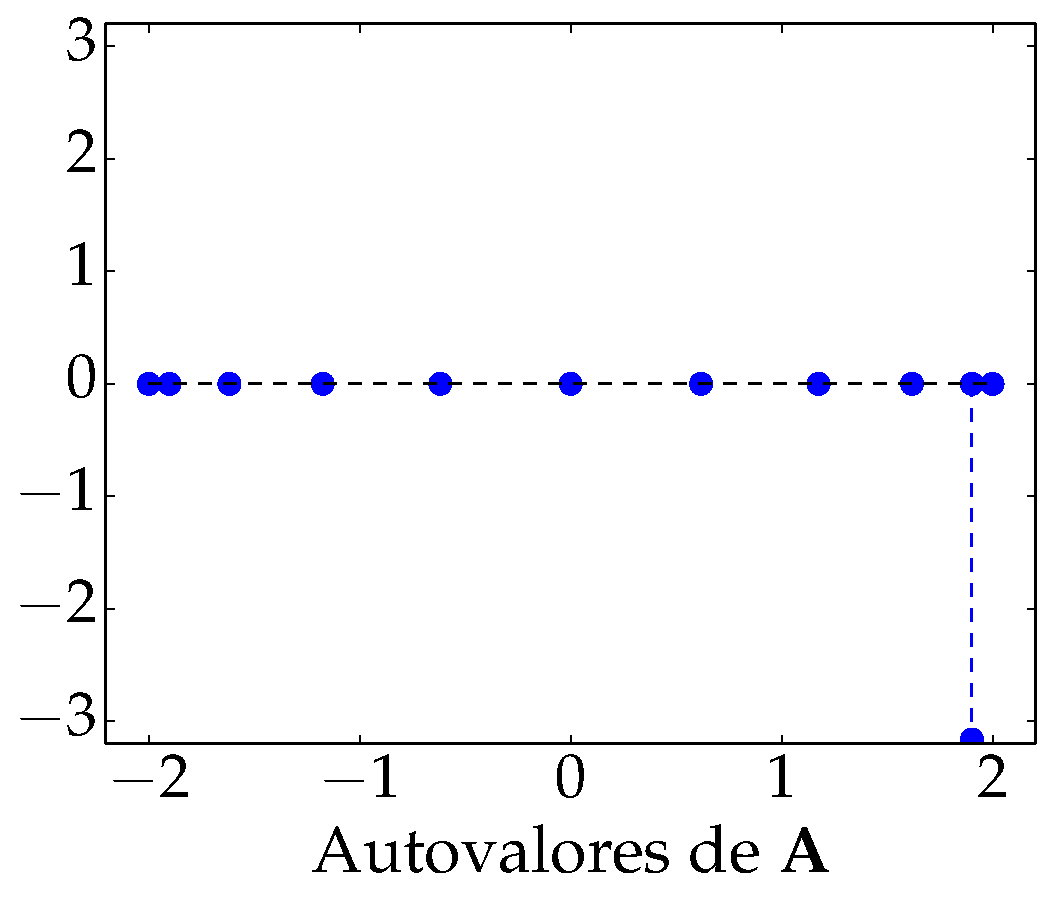
\includegraphics[width=0.35\linewidth]{Figures/ring_different_structure_01_spectrum_GSPA.pdf}
%	}
%	\caption{(a) Sinal sobre um grafo em anel n\~ao-direcionado e (b) seu espectro em GSP\textsubscript{A}.}%
%	\label{fig:diff_struct_GSPA}%
%	\vspace{-0.2cm}
%\end{figure}

\begin{figure}
	\centering
	\begin{minipage}[c]{0.25\linewidth}
		\subfloat[\label{fig:diff_struct_a_GSPA}]{
			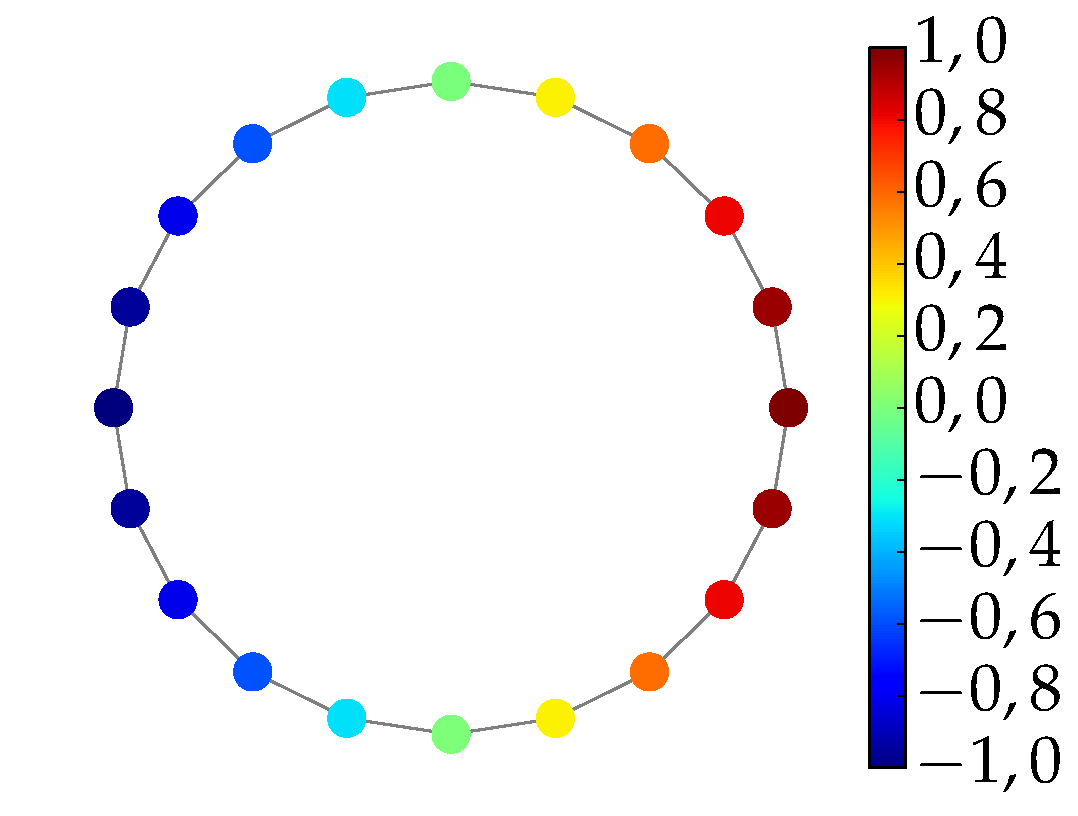
\includegraphics[width=\linewidth]{Figures/ring_different_structure_01_GSPA.pdf}
		}
	\end{minipage}~
	\begin{minipage}[c]{0.25\linewidth}
		\subfloat[\label{fig:diff_struct_b_GSPA}]{
			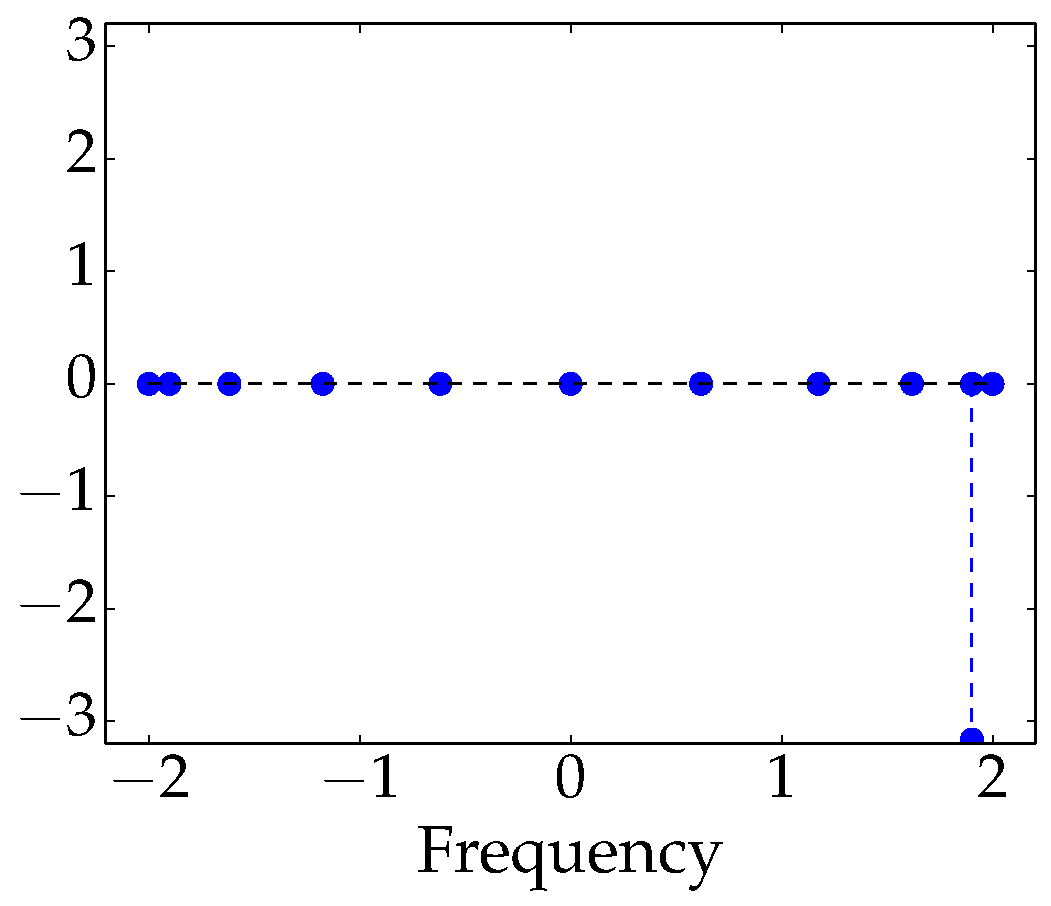
\includegraphics[width=\linewidth]{Figures/ring_different_structure_01_spectrum_GSPA_EN_2.pdf}
		}
	\end{minipage}%
	\caption{(a) Signal defined over an undirected ring graph and (b) its spectrum in the GSP\textsubscript{A} sense, in which the frequency is considered to be the eigenvalues of the adjacency matrix.}%
	\label{fig:diff_struct_GSPA}%
	\vspace{-0.2cm}
\end{figure}

The reader may have noticed a curious consequence from what was previously stated: unless the minimal and characteristic polynomials of $ \mathbf{A} $ are equal, the same frequency may be associated to two or more linearly independent frequency components, as indeed was the case in the example of Fig. \ref{fig:diff_struct_GSPA}. Furthermore, this figure shows that although the signal seems to be smooth, its frequency components are mostly associated with eigenvalues of high magnitude, what is counter-intuitive and provides a motivation to define a clear criterion to distinguish high and low graph frequencies.

The following mathematical reasoning consists of taking a metric which quantifies the expected signal smoothness, and use it to propose or confirm a notion of graph frequency. The metric used by Sandryhaila and Moura was the \emph{total variation}, taken from classical real analysis and defined for differentiable functions as \cite{rudin1987real,mallat1999wavelet}
\begin{equation}
%\label{key}
\Vert f \Vert_V = \int_{-\infty}^{\infty} |f'(t)| \mathrm{d}t.
\end{equation}

For discrete domain functions $ f_N[n] $, the Riemman integral is replaced by first order differences,
\begin{equation}
%\label{key}
\Vert f_N \Vert_V = \sum_p |f_N[n_p + 1] - f_N[n_p]|,
\end{equation}
which clearly quantifies the dissimilarity between contiguous values of the function $ f_N $. With this in mind, it was natural for Sandryhaila and Moura to use this metric in their mathematical formulation of frequency in GSP\textsubscript{A}, wherein they represented the total variation of a finite-length \emph{discrete-time signal} $ \mathbf{x} $ by
\begin{equation}
\label{eq:TV}
TV(\mathbf{x}) = \sum_n | x_n - x_{n-1 \text{ mod } N}|.
\end{equation}

From (\ref{eq:unit_shift}), one can see that (\ref{eq:TV}) may be written in terms of the $ \ell_1 $-norm\footnote{Throughout this paper, the concepts of $ \ell_1 $- and $ \ell_2 $-norm will be frequently used. They are particular cases of the $ \ell_n $-norm of a vector $ \mathbf{x} \in \mathbb{C}^{N} $, defined as $ \Vert \mathbf{x}\Vert_n \overset{\Delta}{=} \left(\sum_{k=0}^{N-1} |x_k|^n\right)^{1/n} $.}
as $ TV(\mathbf{x}) = \Vert \mathbf{x} - \mathbf{C x}\Vert_1 $, by using the directed ring graph adjacency matrix to perform the cyclic shift. From that point, the generalization consisted of using this expression and defining the \emph{total variation on graphs} of a signal $ \mathbf{s} $ defined over the graph $ \mathcal{G} = \{\mathcal{V}, \mathbf{A}\} $ as
\begin{equation}
\label{eq:tv_graphs}
TV_G(\mathbf{s}) \overset{\Delta}{=} \Vert \mathbf{s} - \mathbf{A}^{\text{norm}} \mathbf{s}\Vert_1,
\end{equation}
with $ \mathbf{A}^{\text{norm}} = |\lambda_{max}|^{-1}\mathbf{A} $ and $ \lambda_{max} $ being the eigenvalue of $ \mathbf{A} $ having the highest absolute value. The normalization of the adjacency matrix avoids the excessive magnification of the shifted signal \cite{sandryhaila2014frequency}.

\begin{figure}
	\centering
	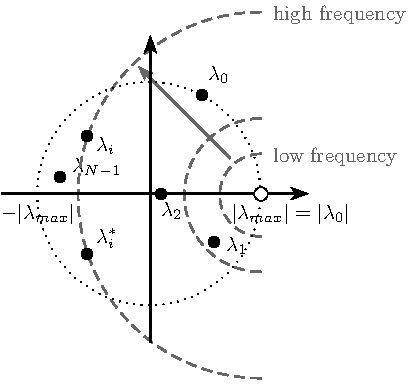
\includegraphics[width=0.35\linewidth]{Figures/graph_frequency_EN.pdf}
	\caption{Frequency ordering of graph signals, from low to high frequencies, in the complex plane \cite{sandryhaila2014frequency}.}
	\label{fig:ordem_freq}
\end{figure}

Let $ \mathbf{A} $ be diagonalizable as in (\ref{eq:gft_01}) with (possibly complex) eigenvalues ordered like so
\begin{equation}
\label{eq:eig_order}
|\lambda_0| \leq |\lambda_1| \leq \dots \leq |\lambda_{N-1}| \overset{\Delta}{=} |\lambda_{max}|,
\end{equation}
associated to the eigenvectors $ (\mathbf{v}_i)_{i=0,\dots,N-1} $, scaled so that $ \Vert \mathbf{v}_i \Vert_1 = 1  \ \forall i$. Taking the total variation (on graphs) of the eigenvector $ \mathbf{v}_k $, one has
\begin{align*}
%\label{key}
TV_G(\mathbf{v}_k) &= \Vert \mathbf{v}_k - \mathbf{A} \mathbf{v}_k \Vert_1  = \Vert\mathbf{v}_k - \frac{1}{|\lambda_{max}|} \lambda_k \mathbf{v}_k \Vert_1 \notag \\
&= \left|1 - \frac{\lambda_k}{|\lambda_{max}|}\right| \Vert \mathbf{v}_k \Vert_1 = \Big| \lambda_k - |\lambda_{max}| \Big| \frac{\Vert \mathbf{v}_k \Vert_{1}}{|\lambda_{max}|}
\end{align*}
so that, since $ \Vert \mathbf{v}_k \Vert_1 = 1 $,
\begin{equation}
\label{eq:TV_ordering}
\Big| \! \lambda_i  - \! |\lambda_{max}|\Big| \! \leq \! \Big|  \lambda_j  - \! |\lambda_{max}|\Big| \! \! \iff \! \! TV_G(\mathbf{v}_i) \leq TV_G(\mathbf{v}_j),
\end{equation}
i.~e. frequency components associated to eigenvalues closer to the real point $ |\lambda_{max}| $ in the complex plane are \emph{smoother} (because they have lower total variation), and therefore are said to be of \emph{low frequency}. Fig. \ref{fig:ordem_freq} illustrates this ordering for graph frequencies, what clarifies the spectrum of the signal in Fig. \ref{fig:diff_struct_a_GSPA} (notice that since the graph is undirected, its adjacency matrix is symmetric and the eigenvalues are real-valued).

%\begin{figure}
%	\centering
%	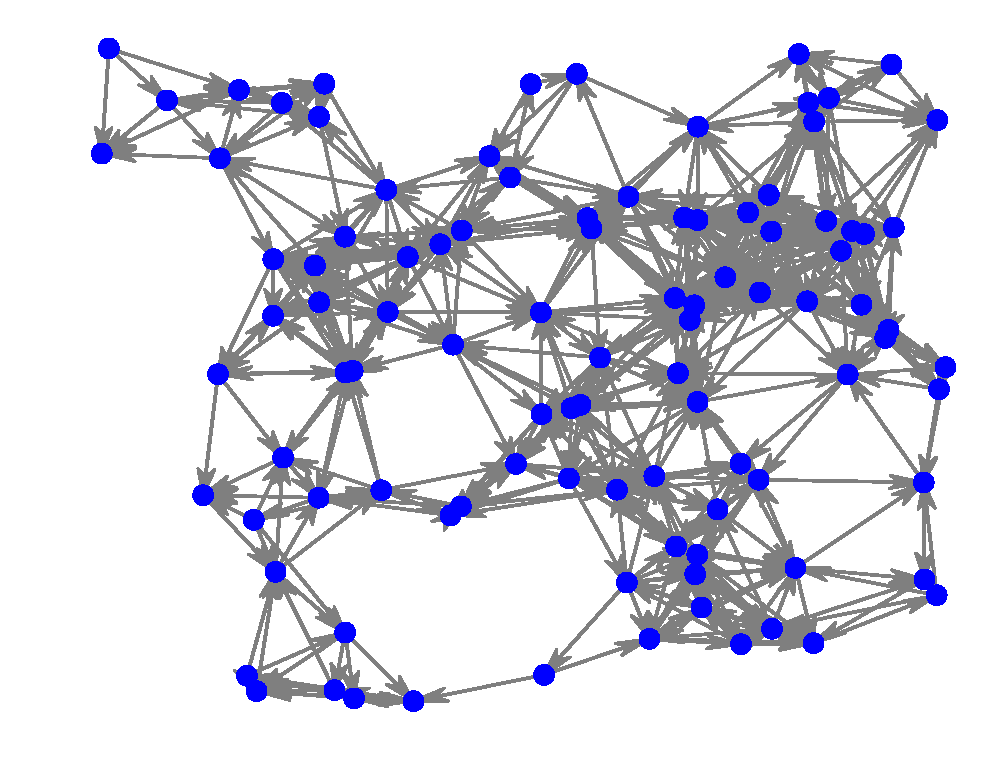
\includegraphics[width=0.6\linewidth]{Figures/showing_random_sensor_spectrum_directed_graph.pdf}
%	\caption{Grafo de sensores direcionado, com 100 v\'ertices, sem la\c cos ou m\'ultiplas arestas.}
%	\label{fig:directed_graph}
%\end{figure}

\begin{figure*}
	\centering
	\subfloat[\label{fig:directed_graph}]{
			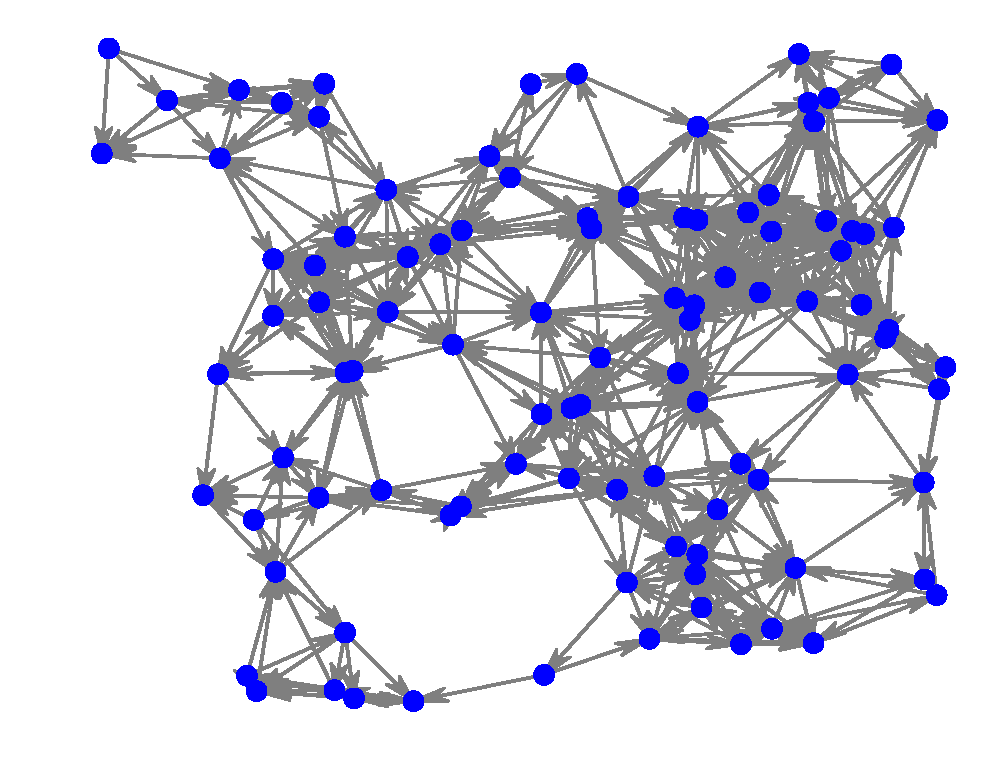
\includegraphics[width=0.33\linewidth]{Figures/showing_random_sensor_spectrum_directed_graph.pdf}
		}
	\subfloat[\label{fig:showing_random_sensor_spectrum_directed_b}]{
		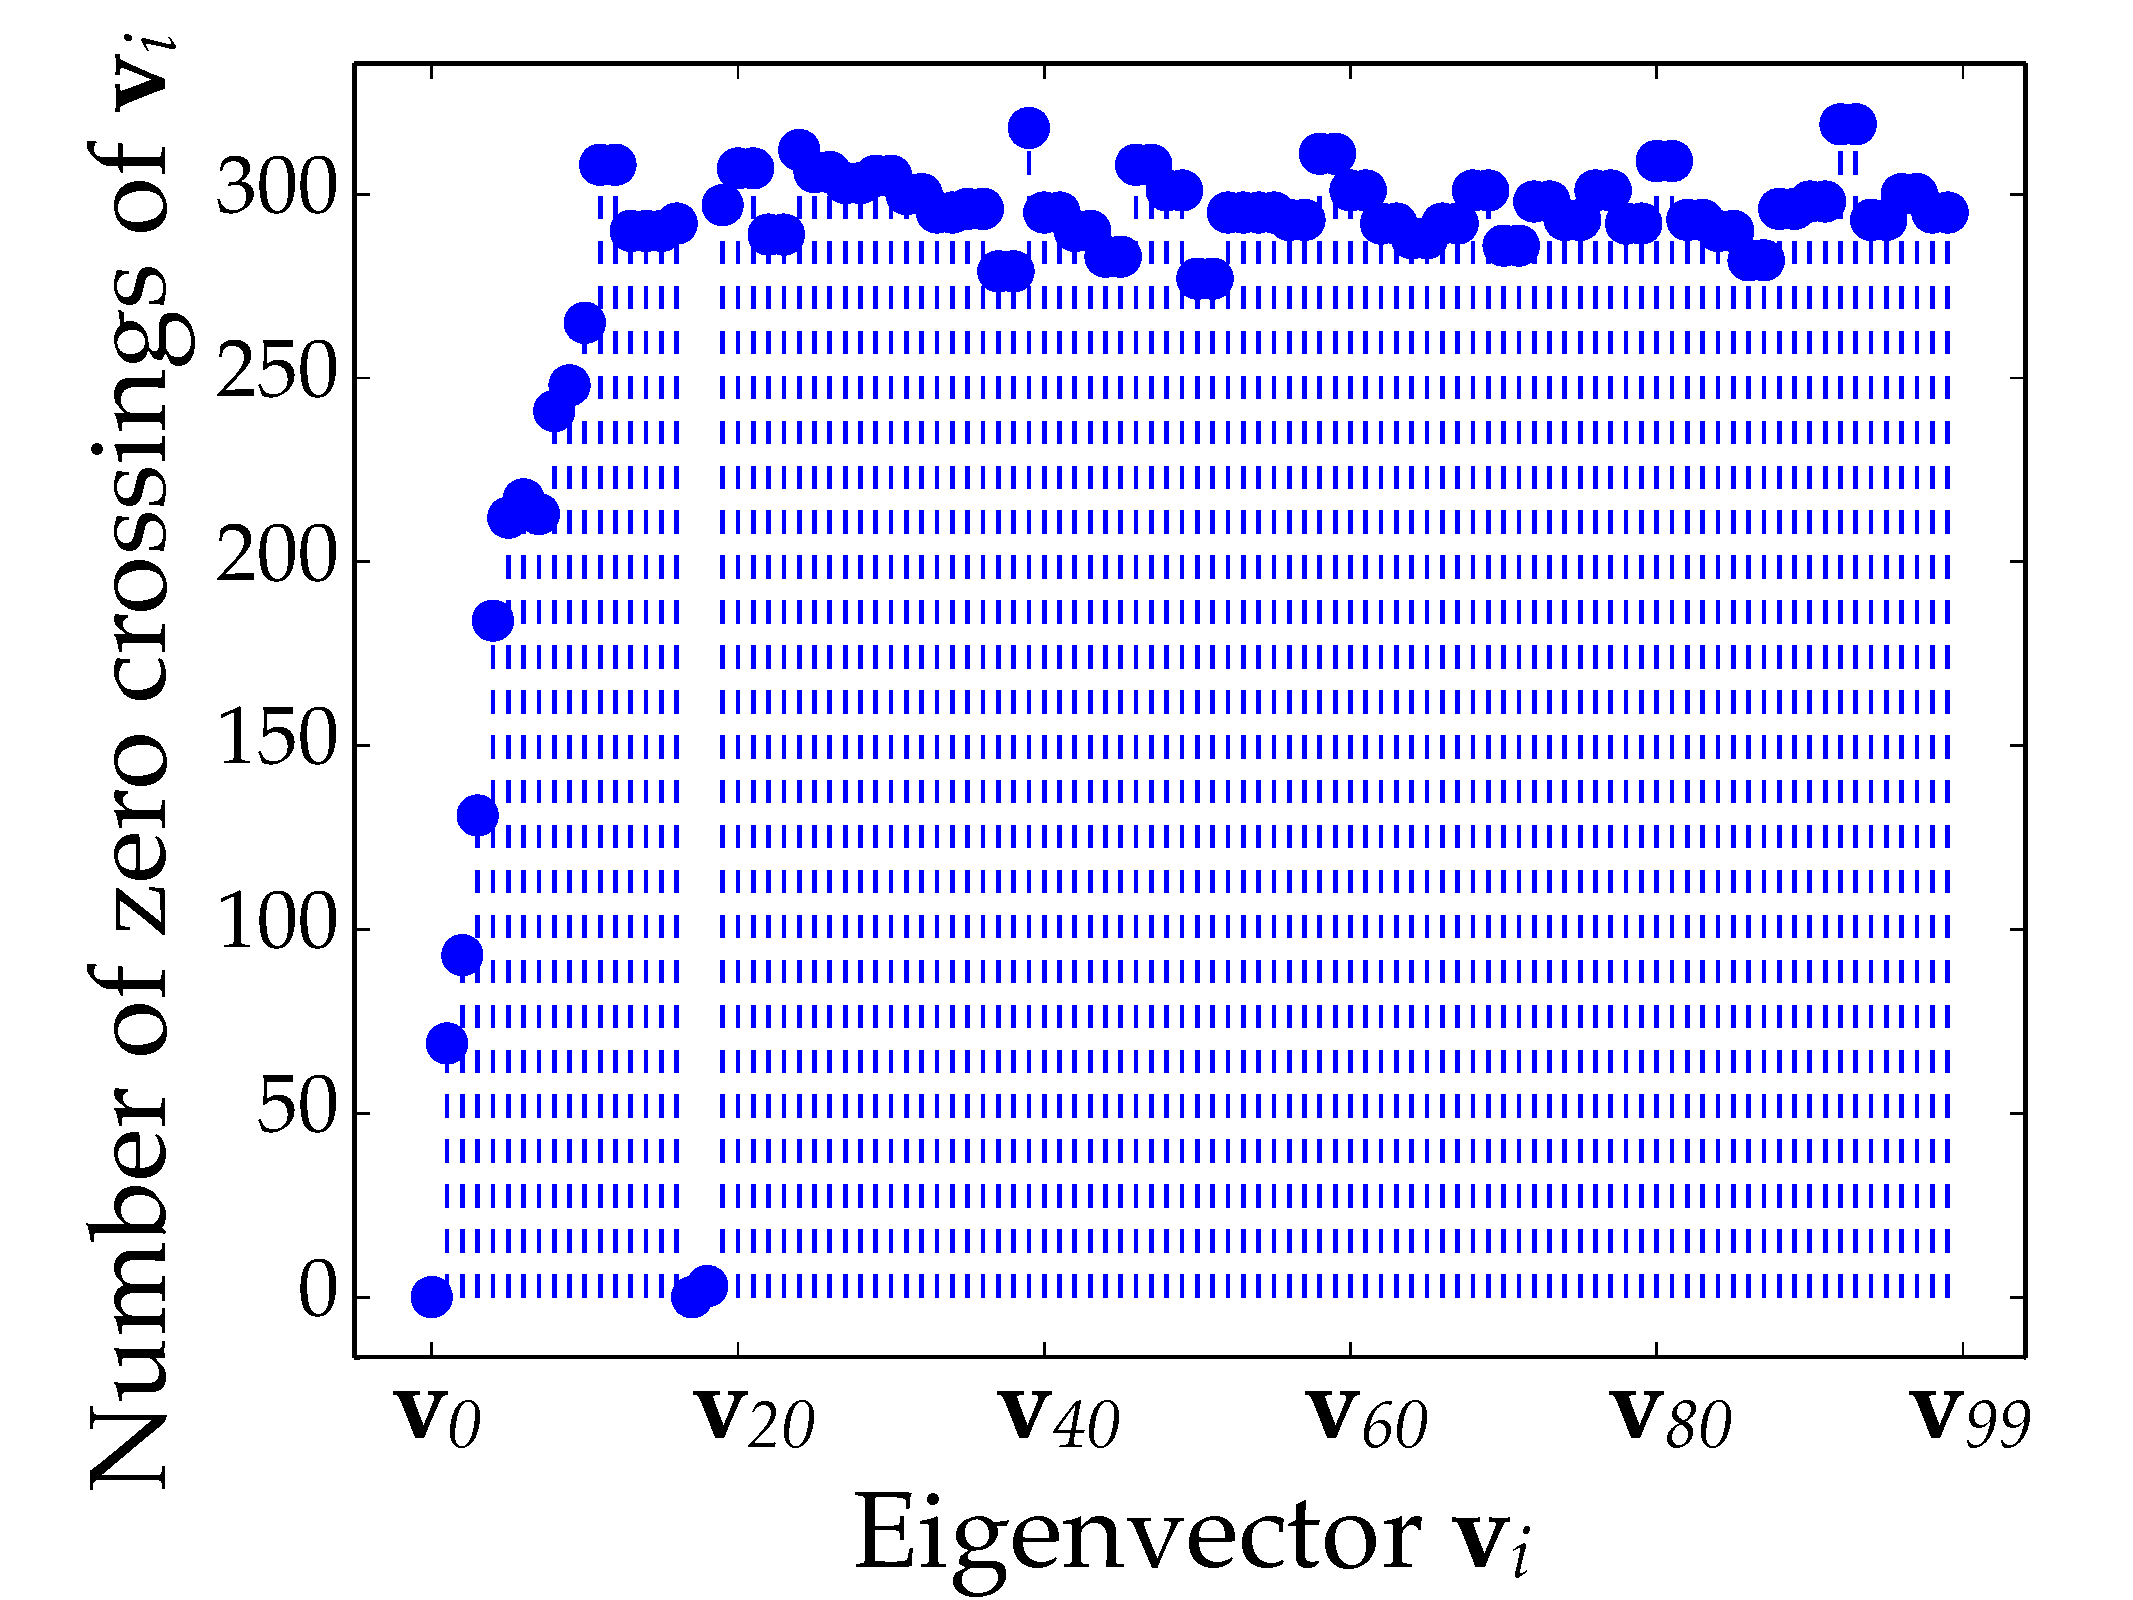
\includegraphics[width=0.33\linewidth]{Figures/showing_random_sensor_spectrum_directed_zero_crossings_1D_edited_EN.pdf}
	}~
	\subfloat[\label{fig:showing_random_sensor_spectrum_directed_c}]{
		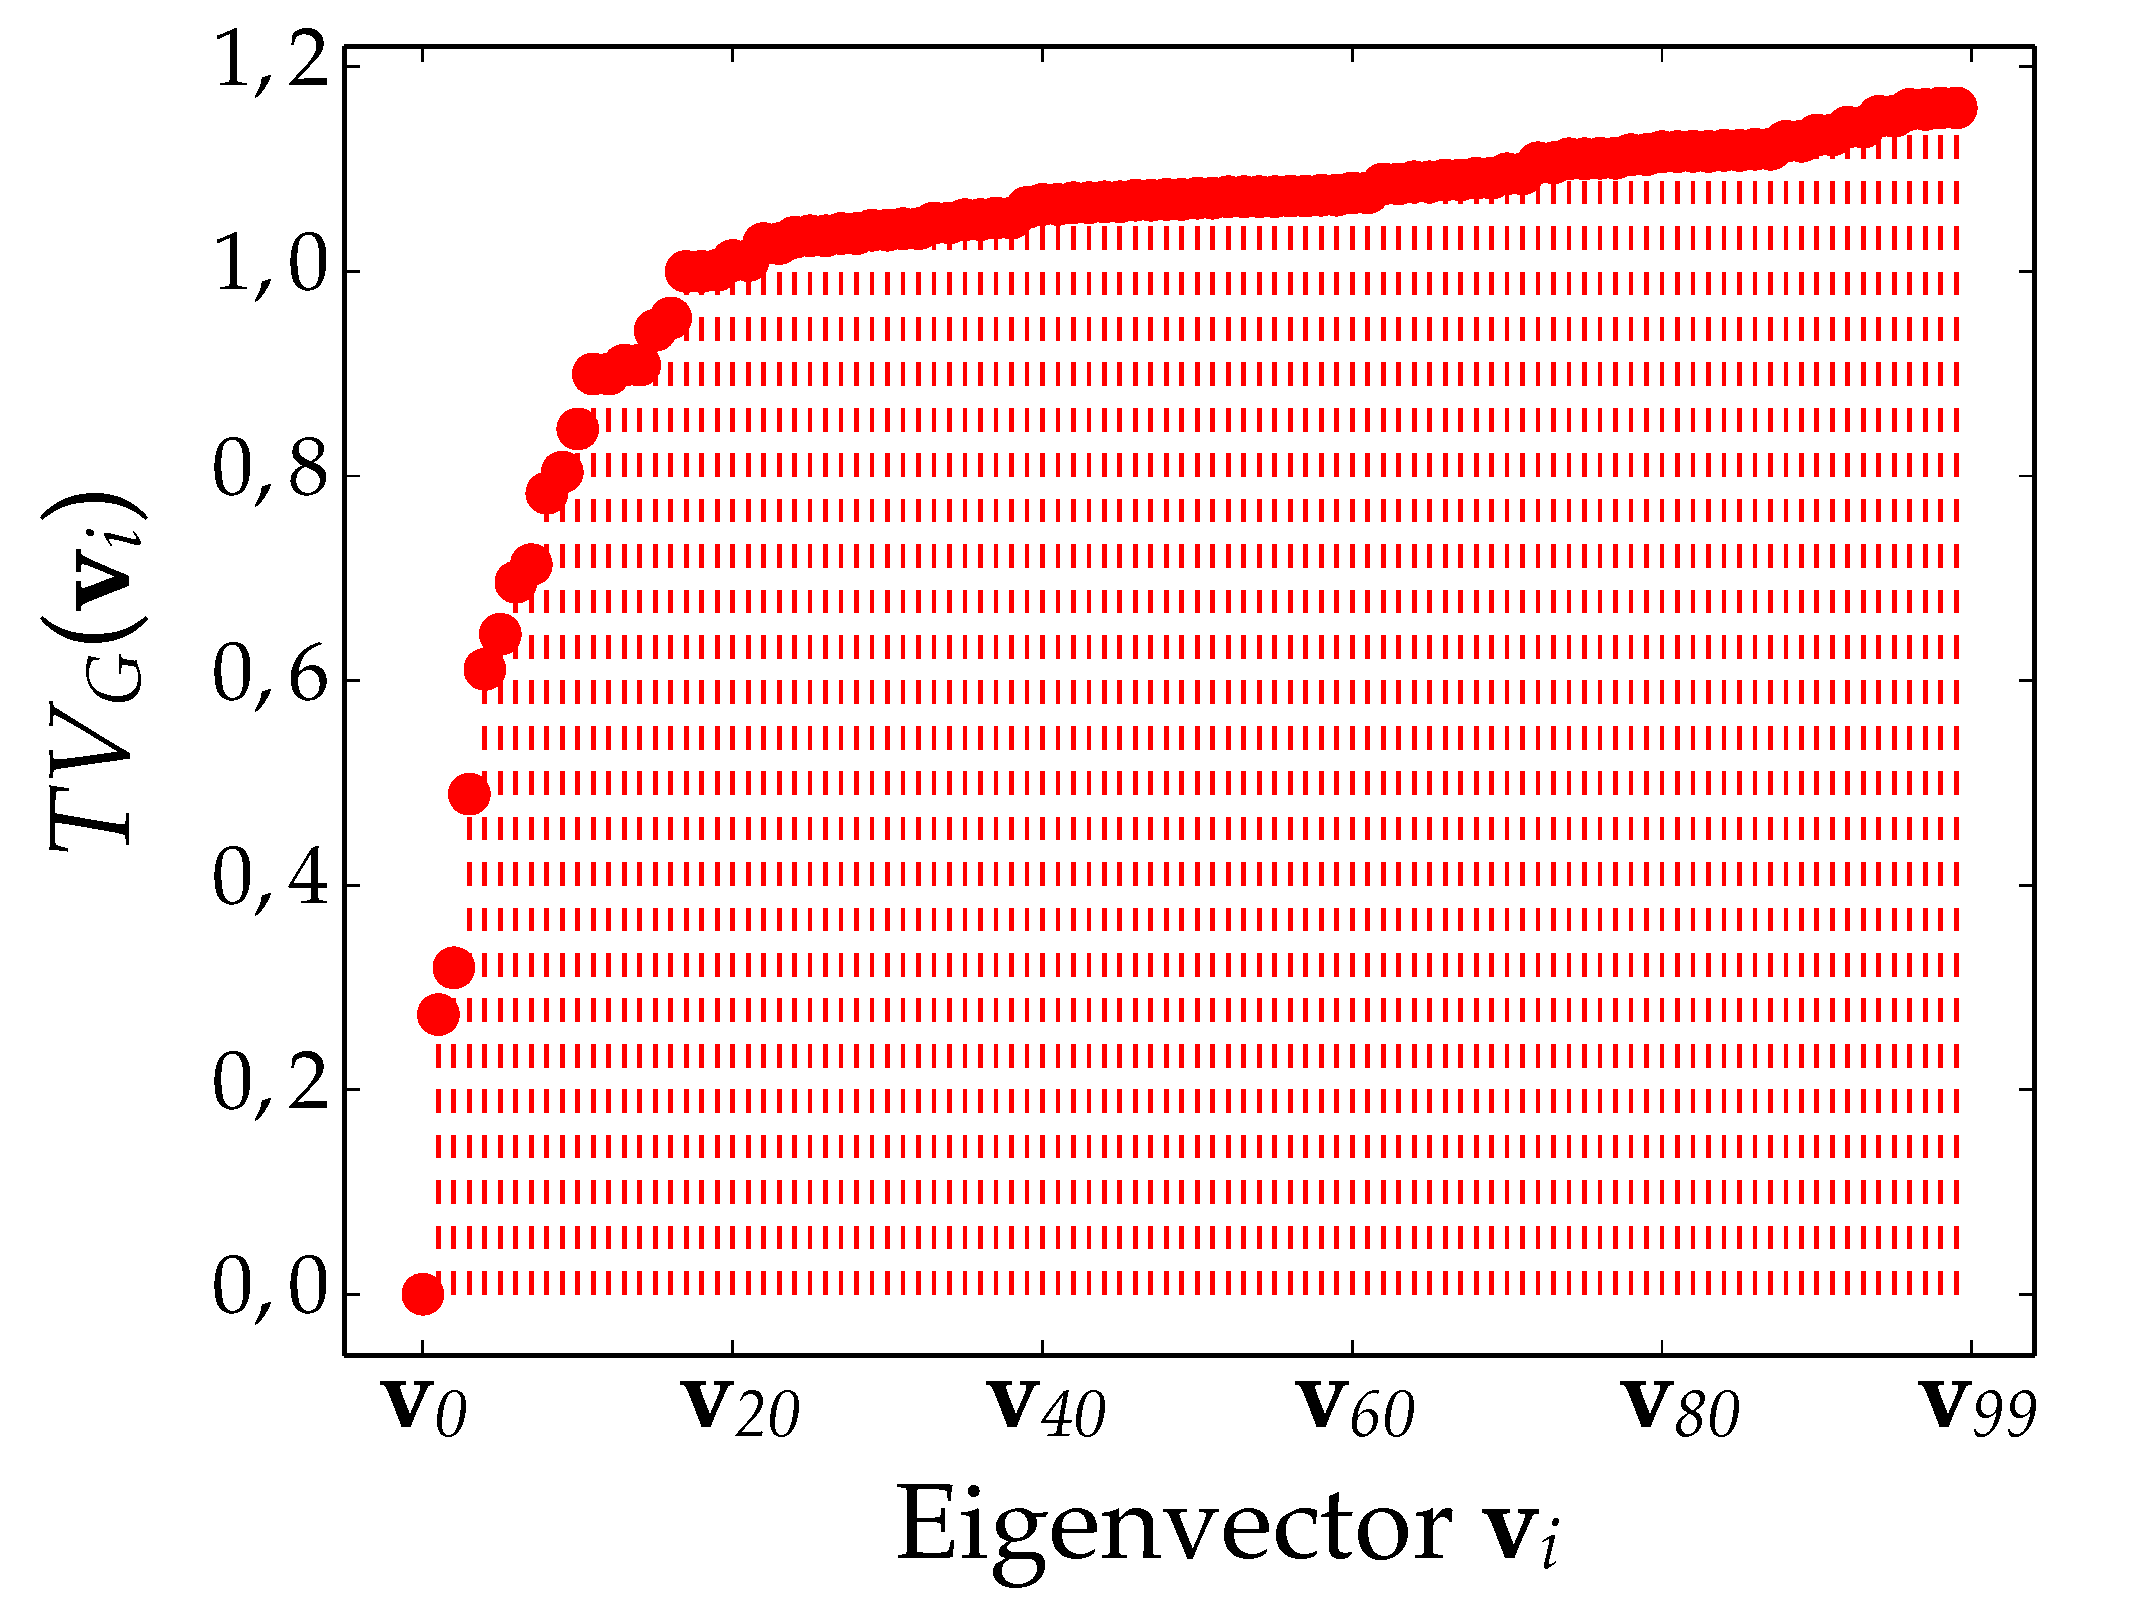
\includegraphics[width=0.33\linewidth]{Figures/showing_random_sensor_spectrum_directed_TV_1D_edited_EN.pdf}
	}
	\caption{(a) Directed sensor graph, with $ N=100 $ vertices and no loops or multiple edges. (b) Number of zero crossings and (b) total variation of the eigenvectors $ (\mathbf{v}_i)_{i=0,\dots,N-1} $ of the adjacency matrix $ \mathbf{A} $ of the graph in \emph{(a)}, ordered so that the respective eigenvalues appear from the closest to the farthest from the real point $ |\lambda_{max}| $ in the complex plane. That is, according to (\ref{eq:TV_ordering}) and Fig. \ref{fig:ordem_freq}, the eigenvectors are disposed in ascending order of frequency.}
	\label{fig:showing_random_sensor_spectrum_directed}
\end{figure*}

Let us take the directed graph in Fig. \ref{fig:directed_graph} to try to verify the consistency of the notion of frequency just derived. For this, along with the total variation on graphs, also the number of zero crossings (i.~e. the number of edges connecting vertices with signal samples of different sign) will be used to \emph{quantify} frequency. This quantity is also related to frequency in classical theory: the more a discrete signal has contiguous samples with different sign, the higher are its frequency components. These two functions, the total variation on graphs and the number of zero crossings, were calculated for each of the adjacency matrix eigenvectors, and the result is shown in Fig. \ref{fig:showing_random_sensor_spectrum_directed}, in which the eigenvectors $ \mathbf{v}_k $ are ordered in such a way that the respective eigenvalues $ \lambda_k $ appear from the closest to the farthest from the real point $ |\lambda_{max}| $ in the complex plane. Both metrics have similar behaviour, but since the number of zero crossings is indifferent to graph signal variations which do not change sign, it was already expected to be less accurate as a figure of merit for frequency. It matters to highlight, however, how the adopted eigenvector ordering indeed implies an ascending frequency order, since both functions in Fig. \ref{fig:showing_random_sensor_spectrum_directed_b} and \ref{fig:showing_random_sensor_spectrum_directed_c} agree on the tendency of growth. More than that, $ TV_G(\mathbf{v}_k) $ grows \emph{monotonically}, as it should do according to (\ref{eq:TV_ordering}).

%It can be seen that both metrics, which are expected to return higher values when having signals with higher frequencies as argument, have similar (but not \emph{equal}) behaviour when evaluated at the eigenvectors $ \mathbf{v}_i $, following what is suggested by (\ref{eq:TV_ordering}) and Fig. \ref{fig:ordem_freq}. However, one can find in Fig. \ref{fig:showing_random_sensor_spectrum_directed} pairs of eigenvectors in which the one expected to have higher frequency appears with lower total variation (notice that the eigenvectors, according to (\ref{eq:TV_ordering}), \emph{should be} in ascending order of frequency). Another curious fact we highlight is that, in both metrics, the eigenvector $ \mathbf{v}_{20} $ and some others have \emph{unexpectedly small values} of total variation and number of zero crossings, what is explicitly shown in Fig. \ref{fig:showing_random_sensor_spectrum_directed_TV_smallest}, in which the 12 smallest values of total variation are shown, among those obtained from all the eigenvectors of $ \mathbf{A} $, as a function of the associated eigenvalues: the eigenvalue with bigger magnitude, in fact, leads to null total variation of its respective eigenvector, but the second smaller total variation is obtained when $ \lambda=0 $. That was not yet fully understood, and further studies are needed to a complete comprehension of the notion of frequency in GSP\textsubscript{A}, and its validity under the metrics used previously.

%\begin{figure}
%	\centering
%	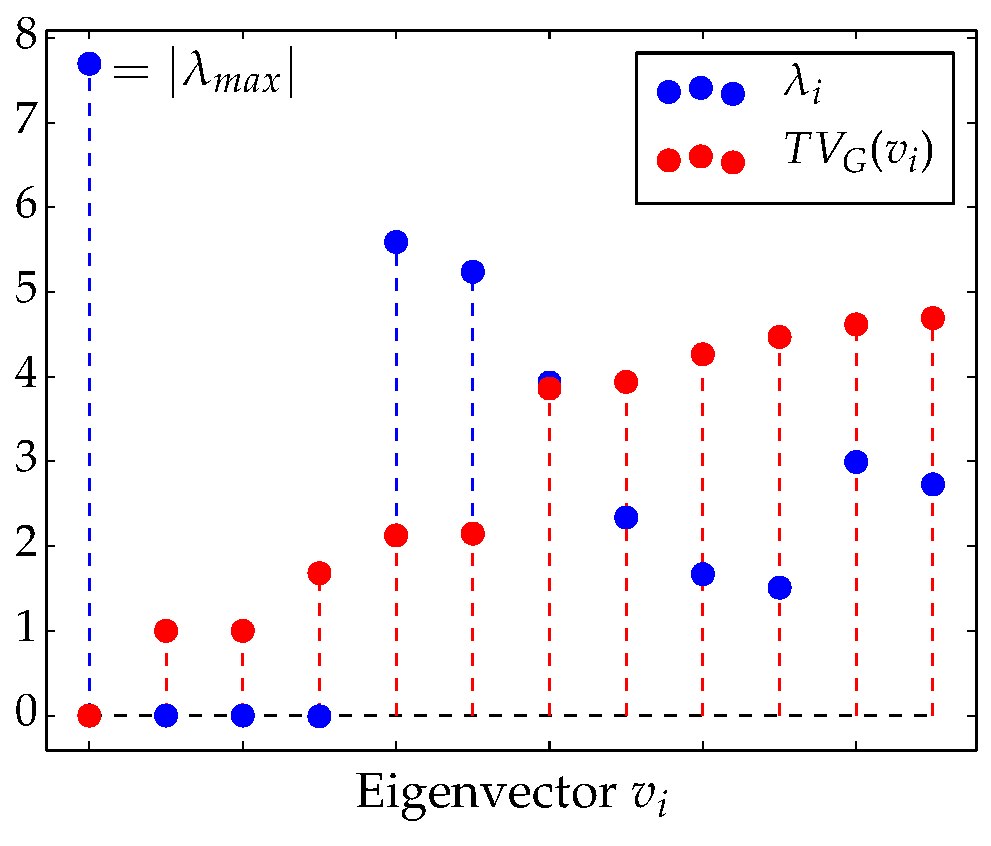
\includegraphics[width=0.65\linewidth]{Figures/showing_random_sensor_spectrum_directed_TV_smallest12_EN.pdf}
%	\caption{The total variation of the adjacency matrix eigenvectors of the graph in Fig. \ref{fig:showing_random_sensor_spectrum_directed} was computed, and the 12 smallest values are shown in red. They are indexed in the horizontal axis by the respective eigenvectors, and the associated eigenvalues are shown in blue.}
%	\label{fig:showing_random_sensor_spectrum_directed_TV_smallest}
%%	\vspace{-0.5cm}
%\end{figure}

It is convenient to conclude this discussion on the graph frequency domain by referring to the frequency response of graph filters. The definition given in Subsection \ref{subsec:filtros} considers the action of a matrix on a signal $ \mathbf{x} $ in the vertex domain of the graph $ \mathcal{G} = \{\mathcal{V}, \mathbf{A}\} $. In order to understand how the filter acts in the GFT domain, hereinafter called frequency domain, one may use (\ref{eq:gft_01}) and the polynomial representation of LSI filters. Let us take the filter $ \mathbf{H} =\sum_{\ell=0}^{L} h_\ell \mathbf{A}^\ell $ and its output to the input $ \mathbf{x} $ given by
\begin{align}\label{eq:resposta_freq_01}
\mathbf{H} \mathbf{x} &= \sum_{\ell=0}^{L} h_\ell \mathbf{A}^\ell \mathbf{x} =
\sum_{\ell=0}^{L} h_\ell \left(\mathbf{V} \mathbf{\Lambda} \mathbf{V}^{-1}\right)^\ell \mathbf{x} \notag \\
&= \mathbf{V} \left(\sum_{\ell=0}^{L} h_\ell \mathbf{\Lambda}^\ell \right) \mathbf{V}^{-1} \mathbf{x}.
\end{align}

Taking the GFT of both sides of the last equation yields
\begin{equation}\label{eq:resposta_freq_02}
\mathbf{V}^{-1} \mathbf{H} \mathbf{x} =
h(\mathbf{\Lambda}) \widehat{\mathbf{x}},
\end{equation}
which indicates that left-multiplication by $ \mathbf{H} $ (action of the filter in the vertex domain) is equivalent to the left-multiplication, in the frequency domain, by the matrix $ h(\mathbf{\Lambda}) $. In other words, $ h(\mathbf{\Lambda}) $ represents the frequency response of $ \mathbf{H} $.


\chapter{The fractional graph shift operator and its applications}
\label{ch:FrGSO}

Over the last decade, theory and applications related to graph signal processing (GSP) have been widely developed and attracted the attention of several scholars~\cite{ortega2018,richard2018,ribeiro2018}. In short, GSP aims to extend concepts and operations of classical digital signal processing (DSP) to scenarios in which the signals lie over irregular domains. Such scenarios include, for instance, sensors arbitrarily positioned in a geographic region and measuring some climatological variable, points of a three-dimensional cloud representing some virtual object and its attributes, people linked according to their interests and proximity relationships in a social network and so on~\cite{chen2014,zhang2014,benzi2016,weiyu2018,saad2018,jiang2021,gama2019,liu2019,zhang2020,ferreira2020,zhang2021,xiao2021,sun2021}. To be more specific, among the issues related to the referred scenarios, one can cite segmentation and attribute compression of 3D point clouds~\cite{zhang2014,zhang2020}, stochastic filtering under asymmetric links in wireless sensor networks~\cite{saad2018}, community detection in social networks~\cite{zhang2021}, anomalous IoT sensor data detection~\cite{xiao2021} and traffic prediction via attention networks~\cite{sun2021}. It is intuitive that the mentioned examples can be modeled as graphs whose vertices are connected by edges inferred from a variety of influence or dependency criteria. This contrasts with the discrete-time domain, over which the samples of a signal are equidistantly placed and have left- and right-side immediate neighbors only; something similar happens in the case of digital images, where the pixels are arranged in a regular rectangular grid.

Two main GSP approaches have been consolidated throughout the last years. The first is based on the spectral graph theory and analyzes signals on undirected graphs with real and non-negative edge weights, by using the graph Laplacian to construct a basis for the signal space~\cite{shuman2013emerging}. The second comes from the algebraic signal processing and uses the weighted adjacency matrix $\mathbf{A}$ as elementary building block~\cite{puschel2008time,puschel2008space}; such an approach, which is adopted in this paper, allows to deal with signals defined over both directed and undirected graphs, and with real- and complex-valued edge weights~\cite{sandryhaila2014big}. \textcolor{black}{In any case, the aforementioned approaches have used $\mathbf{L}$ and $\mathbf{A}$ as elementary building blocks because, among other reasons, these matrices are well established in graph theory and allow some meaningful physical interpretation or some parallel with the classical DSP; while $\mathbf{A}$ can be viewed as a generalization of the discrete-time unit shift, $\mathbf{L}$ is a kind of discrete counterpart to the continuous Laplace-Beltrami (second order) derivative operator on a manifold~\cite{chung1997spectral,Coifman2005}.}

Among the research fronts active in GSP, the one that investigates alternatives to the operators usually employed as building blocks to describe graph signals and systems deserves to be highlighted~\cite{girault2015translation,gavili2017,fan20191,fan2019,mollaebrahim2021,shafipour2018,shafipour2019}. \textcolor{black}{In fact, when the purpose is to consider linear operators in this context, any matrix can be chosen to play the role of elementary building block; multiplying a matrix by a graph signal represented as a vector produces another signal whose samples result from a linear combination of the samples of the original signal. In this scope,} the use of matrices other than the \textit{standard} adjacency matrix and the Laplacian for the mentioned purpose may \textcolor{black}{be more suitable in specific scenarios and to carry out specific (graph) signal processing tasks. Even when the focus is on designing other graph operators (e.g., the graph Fourier transform), the decision about which elementary operator to use has an impact on the expected results.}

\textcolor{black}{Regarding the issue discussed in the last paragraph, some works archived in the GSP literature can be brought to the fore. In~\cite{girault2015translation}, for example, the authors propose an isometric graph translation operator that is described in the spectral domain as a phase shifting operator; this operator shares key properties with the time shift and behaves reasonably in the vertex domain. In~\cite{gavili2017}, the authors define an energy-preserving shift operator that satisfy many properties similar to their counterparts in classical signal processing; the GSP framework based on the referred operator enables the signal analysis along a correlation structure defined by a graph shift manifold. In~\cite{fan20191} and~\cite{fan2019}, the authors employ different features associated with a graph to generate a series of shift operators and design a graph-filter-based classifier. Although the proposed method produces better results than those achieved using conventional graph-filter-based classifiers, it requires dealing with a non-convex optimization problem whose solution involves a relatively high computational cost. In~\cite{mollaebrahim2021}, motivated by the typical scenario of asymmetric communications in wireless sensor networks, the authors study the optimal design of graph shift operators to perform decentralized subspace projection for asymmetric topologies. Obtaining the referred operators can be performed either by solving an optimization problem or by employing a decentralized algorithm based on an Alternating Direction Method of Multipliers (ADMM). In~\cite{shafipour2018} and~\cite{shafipour2019}, the goal is to construct a graph Fourier transform for directed graphs (digraphs), such that the corresponding orthonormal frequency components are as spread as possible in the graph spectral domain. The method uses the Laplacian of an undirected version of the digraph and involves non-convex, orthonormality-constrained optimization problems.} 

\textcolor{black}{This paper is somehow related to the above mentioned works, since its central theme refers to elementary operators on graphs. To be more specific, we consider the} possibility of \textcolor{black}{computing} a non-integer power $\mathbf{A}^a$, $a\in\mathbb{R}$, of the adjacency matrix $\mathbf{A}$, \textcolor{black}{which is taken as} the (unit) graph shift operator~\cite{sandryhaila2014big}. \textcolor{black}{With this,} we introduce the notion of fractional shift (or delay) of signals on graphs, \textcolor{black}{which, to the best of our knowledge, has not yet been addressed in the literature. Differently from the referred papers, in which new operators are created or standard operators are adjusted using strategies potentially expensive from the computational point of view, we propose a relatively simple generalization that fills a theoretical gap concerning the extension to the GSP framework of a well-established concept in the classical signal processing.}

\color{black}
In what follows, the main contributions of this paper are listed:
\begin{itemize}
\item We introduce the fractional graph shift operator $\mathbf{A}^a$ and discuss its several aspects. More specifically, we demonstrate that $\mathbf{A}^a$ can be computed by using the theory of matrix functions, considering the Jordan decomposition of $\mathbf{A}$.
\item We demonstrate that $\mathbf{A}^a$ acts as a graph filter, give its frequency response and discuss issues related to fractionally shifting graph signals containing descontinuities (Gibbs phenomenon).

\item An analogy between the proposed graph fractional operator and that considered in the classical discrete-time case is established; our result suggests that, when a directed ring graph with $N$ vertices is considered, the response of the corresponding graph filter related to $\mathbf{A}^a$ converges to that of the classical fractional delay filter as $N$ grows.

\item We determine the polynomial representation of $\mathbf{A}^a$ and, with that, we demonstrate that, for any graph, such an operator can be implemented as a linear and shift-invariant (LSI) graph filter.
\end{itemize}

This paper is organized as follows. Section~\ref{sec:revgsp} contains a concise review of graph signal processing foundations. In Section~\ref{sec:fracshift}, we introduce the concept of fractional shift on graphs and develop our contributions in detail: we address the computation of $\mathbf{A}^a$ in Subsection~\ref{subsec:comp}, discuss its interpretation in Subsection~\ref{subsec:interpret}, demonstrate its consistency with the ideal fractional delay filter in Subsection~\ref{subsec:consist} and determine its polynomial representation in Subsection~\ref{subsec:poly}. Section~\ref{sec:num} is devoted to numerical results related to the developed theory: we first present a small example regarding the polynomial representation of $\mathbf{A}^a$ in Subsection~\ref{subsec:num1}; we then consider a real-world graph signal (temperature measured by weather stations) and demonstrate that, using $\mathbf{A}^a$, we can obtain filters that  approximate an ideal filter (in the least-squares sense) better than those designed using $\mathbf{A}$ (Subsections~\ref{subsec:lsi} and~\ref{subsec:lsi01}); finally, this possibility is illustrated by means of an example involving the noise removal from the same graph signal (Subsection~\ref{subsec:lsi02}). The paper closes with concluding remarks in Section~\ref{sec:conc}.

\color{black}
\section{Foundations of Graph Signal Processing}\label{sec:revgsp}
In this section, the main concepts and definitions related to GSP are briefly presented. As previously remarked, the GSP framework considered in this paper is the one based on the adjacency matrix. In this sense, if one wishes for a deeper introduction on the matter, please refer to the works of Sandryhaila, Moura \emph{et al.} \cite{chen2015,sandryhaila2013discrete,sandryhaila2013filters,sandryhaila2013gft,sandryhaila2014big,sandryhaila2014frequency}.

\subsection{Graph Signals and Filters}
Let $ \mathcal{G} = \{\mathbf{A}, \mathcal{V}\} $ be a graph defined as a set of vertices $ \mathcal{V} = \{v_0, v_1, \dots, v_{N-1}\}$ possibly connected by weighted edges. The adjacency matrix $ \mathbf{A} $ has in its entry $ A_{ij} $ the weight of the edge going from $ v_j $ to $ v_i $, with $A_{ij} = 0 $ if and only if there is no edge from $ v_j $ to $ v_i $.

A signal $ \mathbf{x} \in \mathcal{S}$ over the graph $ \mathcal{G} $ is defined as
\begin{align}\label{eq:def_sinal}
\mathbf{x}: \ \ &\mathcal{V} \rightarrow \mathbb{C}^{N}, \notag \\
& v_n \rightarrow \mathbf{x}(v_n) = x_n,
\end{align}
where $ \mathcal{S} $ is the space of all signals over $ \mathcal{G} $, that is, the space of discrete functions mapping the set of the $ N $ vertices of $ \mathcal{G} $ into an $ N $-tuple of complex (or real) values. Given a suitable labelling for the vertices of a graph, a signal $ \mathbf{x} $ is represented by the ordered sequence $x_n$ of its values. Graph signals can then be written as ordered $ N $-tuples lying in $ \mathbb{C}^N $ or $ \mathbb{R}^N $.%, cabendo aqui lembrar que a esta representa\c{c}\~ao est\'a ligada necessariamente uma rotula\c{c}\~ao espec\'ifica dos v\'ertices do grafo sobre o qual se define o sinal.

Graphs can be \emph{directed} or \emph{undirected}, depending on whether their edges have or do not have preferred direction. By definition, an adjacency matrix is symmetrical if and only if the corresponding graph is undirected.

A particularly important graph is that shown in Fig.~\ref{fig:graphs}, the directed ring graph with edges having unitary weights. Such a graph can be used to model the discrete-time domain with length $N$ and periodic boundary conditions. Its adjacency matrix is given by
%\begin{figure}%
%	\centering
%	\subfloat[\label{figa_graphs}]{{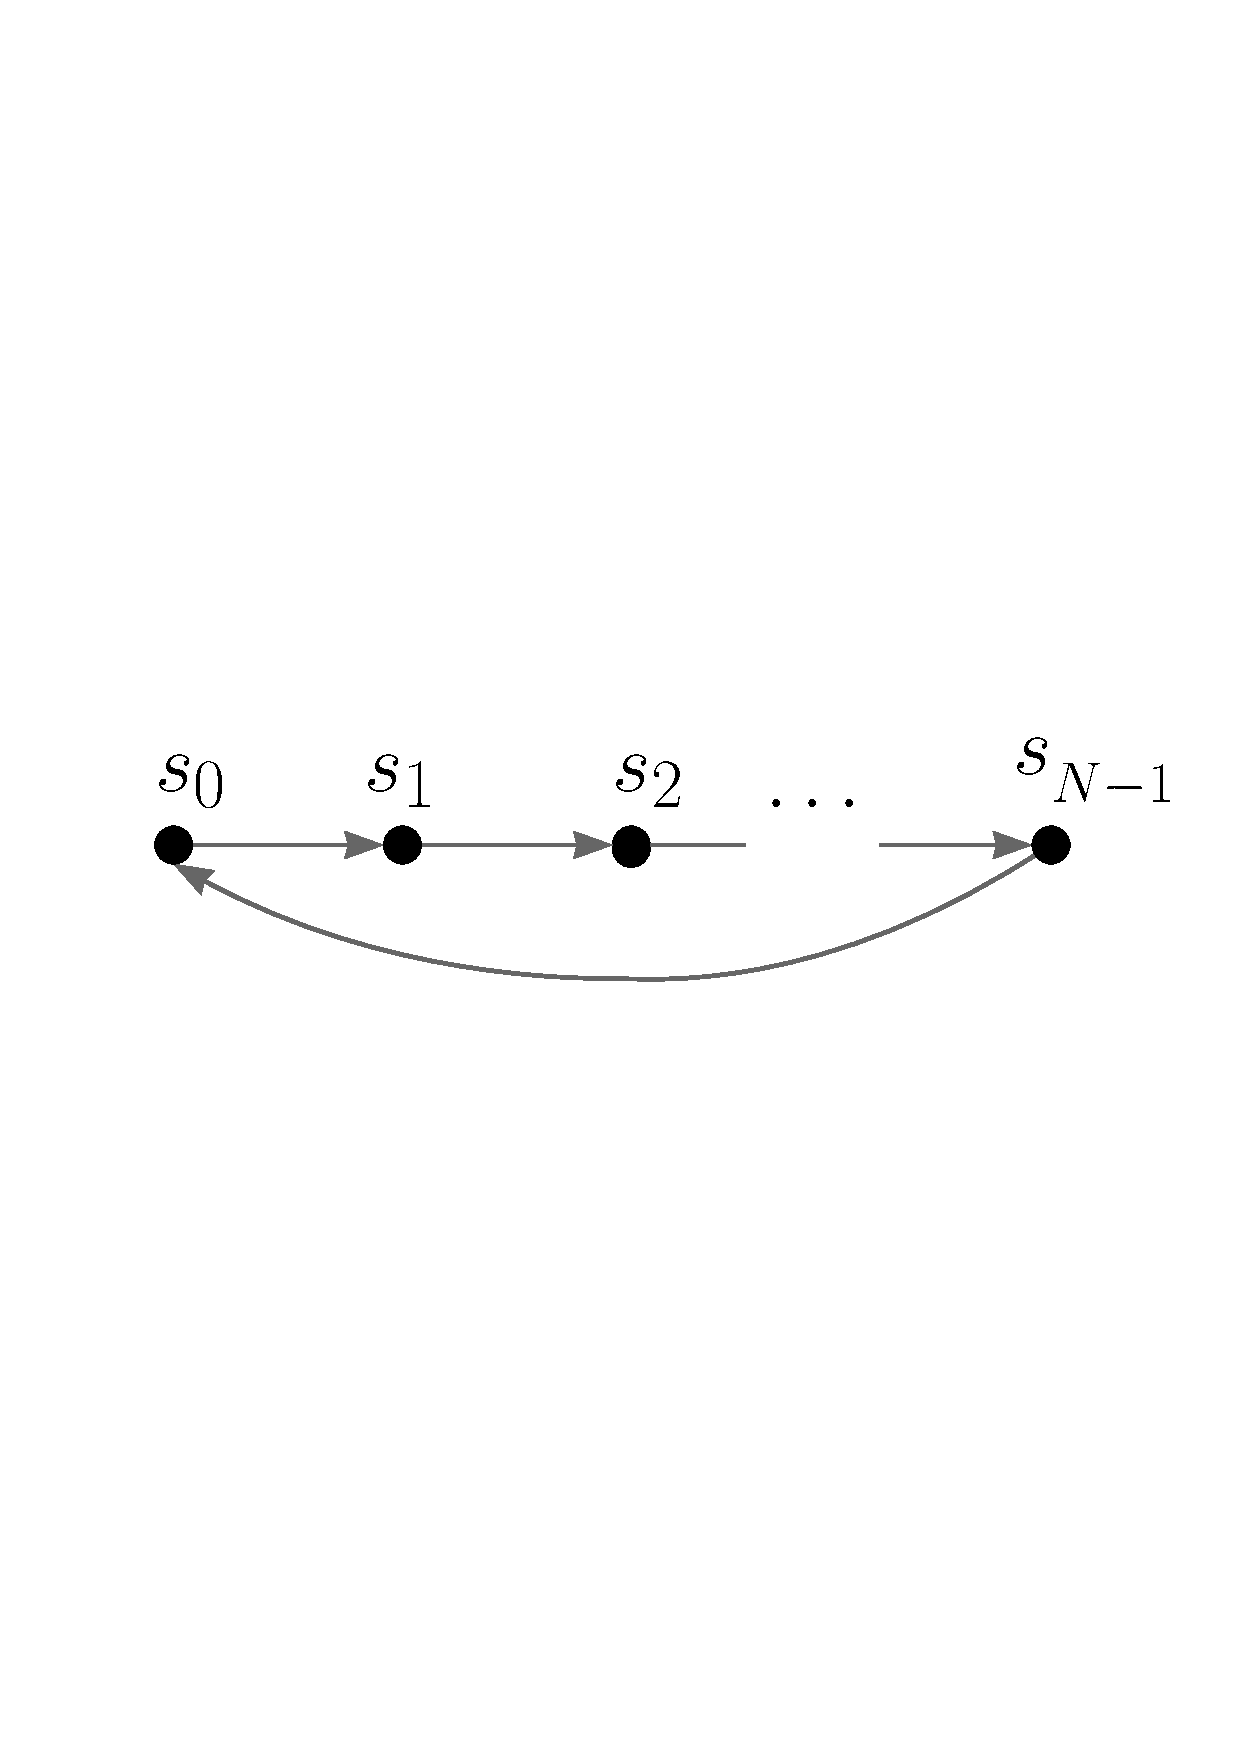
\includegraphics[width=0.45\linewidth]{Figures/signal_ring_graph_white_border.pdf} }}\hspace{0.2cm}%
%	\qquad
%	\subfloat[t][\label{figb_graphs}]{{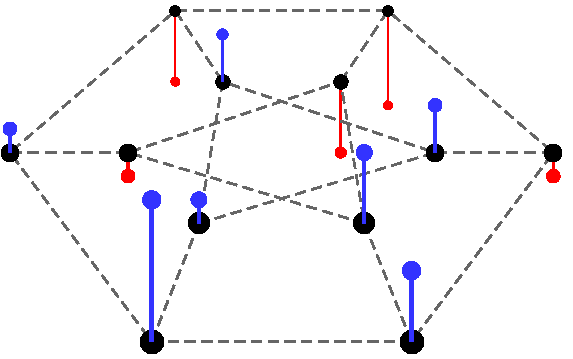
\includegraphics[width=0.4\linewidth]{Figures/signal_duher_graph.pdf} }}\\
%	\subfloat[\label{figc_graphs}]{{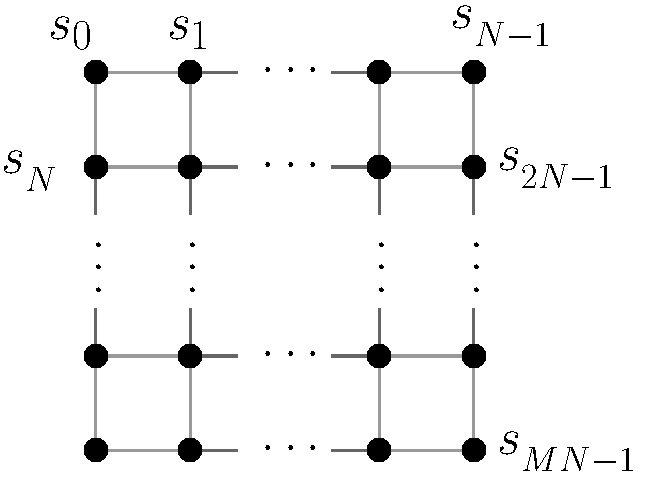
\includegraphics[width=0.45\linewidth]{Figures/image_graph.pdf} }}%
%	\subfloat[\label{figd_graphs}]{{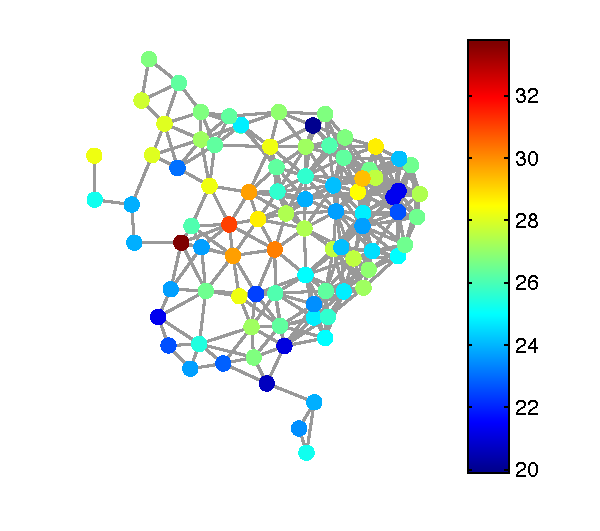
\includegraphics[width=0.4\linewidth]{Figures/graph_temp_bulbo_seco_NE_00h_01Fev2012_cropped.pdf} }}%
%	\caption{Exemplos de representa\c{c}\~oes de sinais sobre (a) um grafo em anel direcionado, (b) um grafo de D\"{u}her n\~ao-direcionado, (c) um grafo n\~ao-direcionado em forma de rede retangular uniforme  e (d) um grafo formado por cidades do Nordeste brasileiro.}%
%	\label{fig:graphs}%
%	\vspace{-0.2cm}
%\end{figure}
\begin{equation}\label{eq:C}
\mathbf{C} =
\begin{bmatrix}
&  &  &   1\\ 
1 &  &   & \\ 
&   \ddots &  & \\ 
&  &   1 & 
\end{bmatrix},
\end{equation}
\noindent and plays an essential role in GSP: if a signal $ \mathbf{x} = (x_0 \ x_1 \ \dots \ x_{N-1})^T $ defined on a ring graph is left multiplied by the adjacency matix, one has $ \widetilde{\mathbf{x}} = (s_{N-1} \ x_0 \ \dots \ s_{N-2})^T $; that is,
\begin{equation}\label{eq:graph_shift_C}
\widetilde{\mathbf{x}} = \mathbf{C} \mathbf{x}
\end{equation}
\noindent is the result of circularly shifting $ \mathbf{x} $ to the right. This property suggests to generalize the unit shift of a signal on an arbitrary graph as being the left product by the corresponding adjacency matrix,
\begin{equation}\label{eq:graph_shift_A}
\widetilde{\mathbf{x}} = \mathbf{A} \mathbf{x},
\end{equation}
\noindent so that $ \mathbf{A} $ can be interpreted as the graph shift operator. In fact, this operator is a delay \emph{filter} for graph signals.

A filter for signals on a graph with $ |\mathcal{V}| = N $ vertices can be defined as being any matrix $ \mathbf{H} \in \mathbb{C}^{N \times N} $ \cite{sandryhaila2013discrete}. Therefore, every graph filter is linear. On the other hand,
\begin{equation}\label{eq:shift_invariance}
\mathbf{HA}\mathbf{x} = \mathbf{AH}\mathbf{x},\:\:\forall \mathbf{x} \in \mathcal{S} \:\:\Leftrightarrow\:\:\mathbf{HA} = \mathbf{AH},
\end{equation}
\noindent that is, $ \mathbf{H} $ is a linear and shift-invariant (LSI) filter if and only if it commutes with the adjacency matrix $ \mathbf{A} $. The following theorem establishes an important property satisfied by every LSI filter~\cite{sandryhaila2013discrete} .
\vspace{0.2cm}
\begin{theorem}
	\label{theo:01}
	Let $ \mathbf{A} $ be the adjacency matrix of a graph. Let us assume that the characteristic polynomial $char_{\mathbf{A}}(x)$ of $\mathbf{A}$ coincides with the respective minimal polynomial $m_{\mathbf{A}}(x) $. Therefore, $ \mathbf{H} $ is a LSI filter if and only if $ \mathbf{H} $ is a polynomial in $ \mathbf{A} $, i.~e.
	\begin{equation}\label{eq:filtro}
	\mathbf{H} = h(\mathbf{A}) = \sum_{\ell=0}^{L} h_\ell \mathbf{A}^\ell,
	\end{equation}
where $ \mathbf{A}^0 $ is the identity matrix and $ L < \deg(m_{\mathbf{A}}) $.
\end{theorem}

The assumption on $char_{\mathbf{A}}(x)$ and $m_{\mathbf{A}}(x)$ in Theorem~\ref{theo:01} does not hold for all adjacency matrices $\mathbf{A}$. Nevertheless, the result in the referred theorem can be extended to all matrices using the concept of \emph{equivalent graph filters}, as clearly explained in~\cite{sandryhaila2013filters}. In short, for any graph $\mathcal{G} = \{\mathbf{A}, \mathcal{V}\}$, every LSI filter has polynomial representation in $\mathbf{A}$. In this sense, Theorem~\ref{theo:01} suggests a convenient analogy with the classical DSP, since every filter for discrete-time signals can be represented as polynomials evaluated in $ z^{-1} $, the unit delay, via the $z$-transform of its impulse response.

\begin{figure}[t!]
	\centering
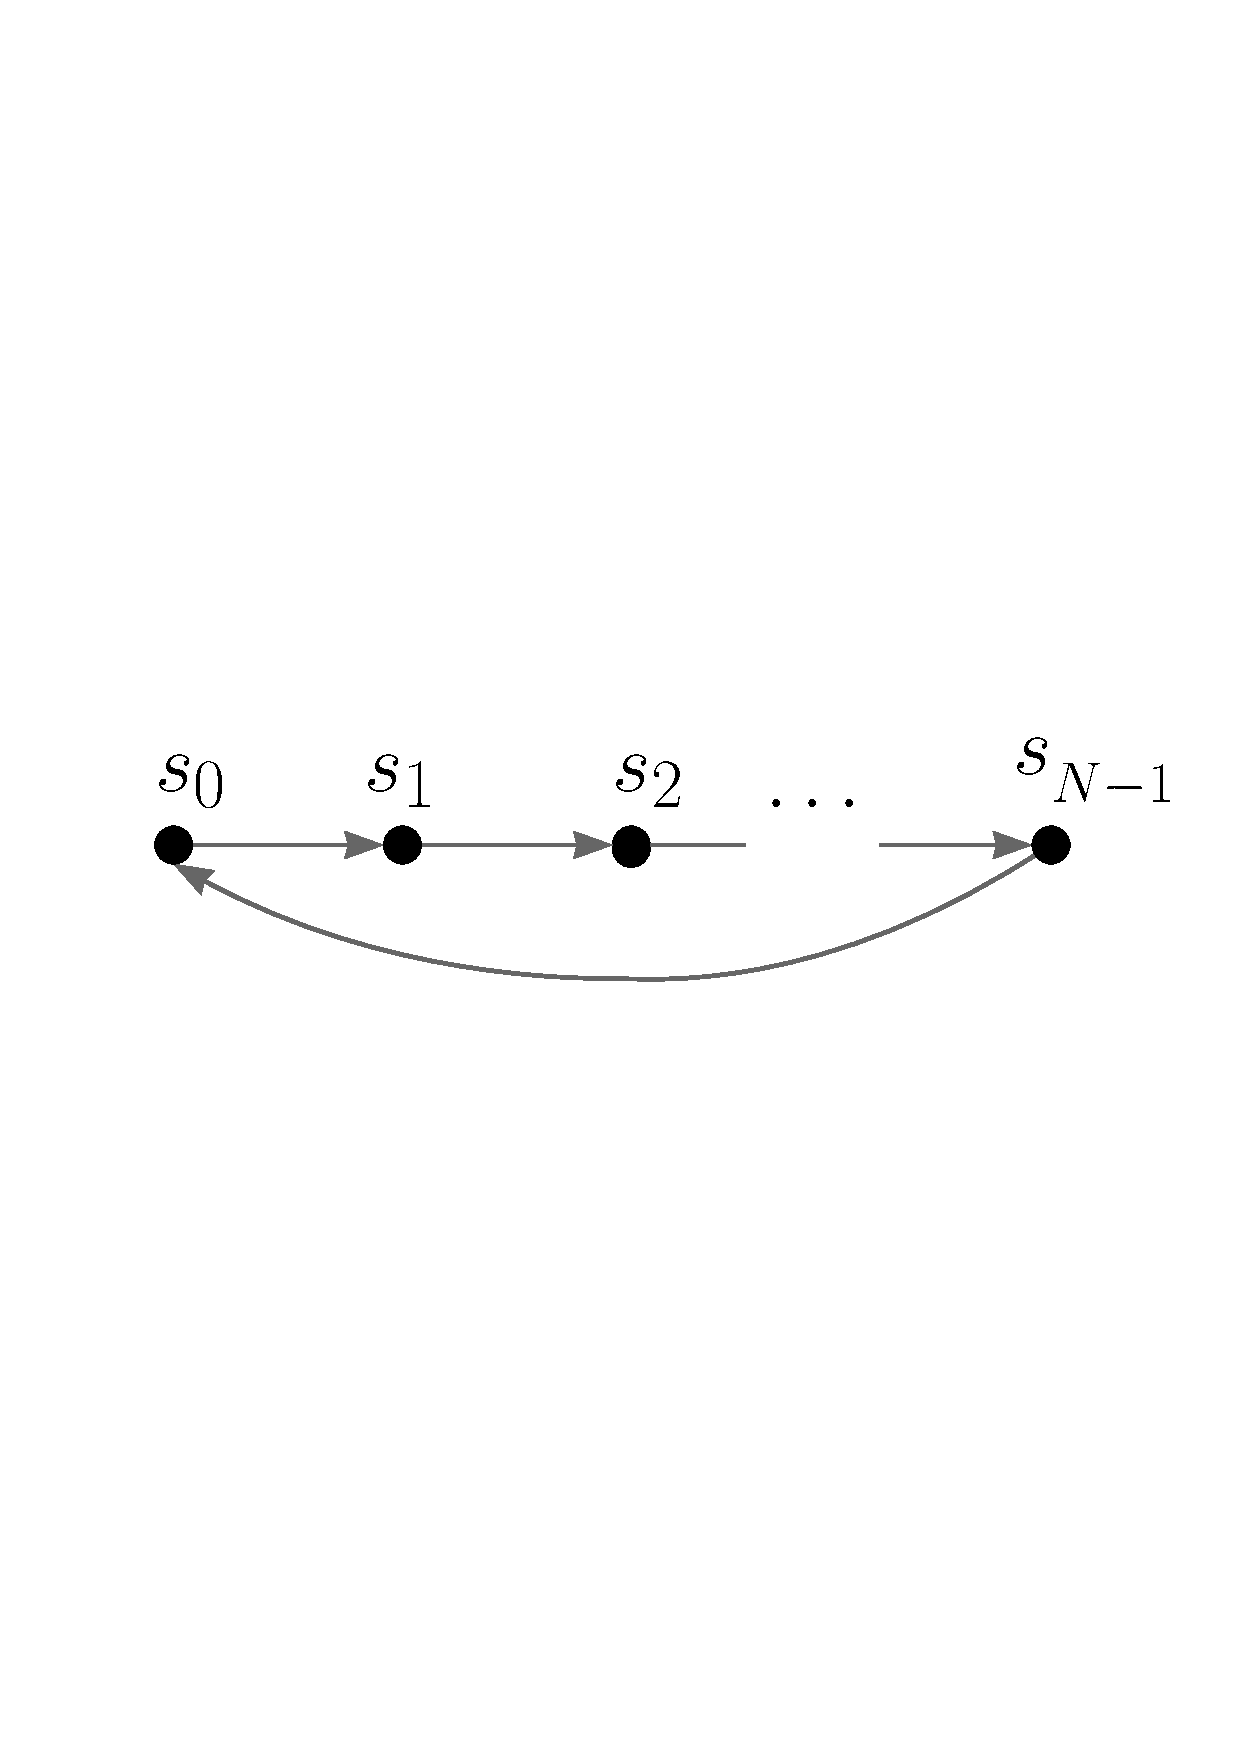
\includegraphics[width=0.3\linewidth]{Figures/signal_ring_graph_white_border.pdf}
	\caption{A directed ring graph.}%
	\label{fig:graphs}%
	\vspace{-0.5cm}
\end{figure}
\subsection{Graph Fourier Transform}

The graph Fourier transform of a signal is its projection on a basis formed by functions invariant to linear and time-invariant (LTI) filtering~\cite{oppenheim1997signals}. Analogously, the graph Fourier transform (GFT) can be defined as the decomposition of a signal on a basis formed by eigenvectors of LSI filtering. Since LSI filters are polynomials in $ \mathbf{A} $ (Theorem \ref{theo:01}), and considering that a matrix and its integer powers share the same eigenvectors, the referred basis coincides with that obtained from the decomposition of $\mathbf{A}$~\cite{sandryhaila2013gft}. In this context, if the corresponding graph has $ N $ vertices, $\mathbf{A} $ admits the Jordan decomposition
\begin{equation}\label{eq:gft_01}
\mathbf{A} = \mathbf{V} \mathbf{J} \mathbf{V}^{-1},
\end{equation}
in which $ \mathbf{V} $ contains the $ N $ Jordan (generalized) eigenvectors of $ \mathbf{A} $ in its columns,
\begin{equation}\label{eq:gft_02}
\mathbf{V} = \left(\mathbf{v}_0 \ \mathbf{v}_1 \ \dots\ \mathbf{v}_{N-1}\right),
\end{equation}
and $\mathbf{J}$ is a block diagonal matrix formed of the so-called Jordan blocks. In particular, if $\mathbf{A}$ is diagonalizable, (\ref{eq:gft_01}) coincides with its eigendecomposition, so that $\mathbf{J}$ reduces to a diagonal matrix whose entries are the eigenvalues of $\mathbf{A}$.

%Additionally, the subspaces generated by the eigenvectors of a given eigenvalue of $ \mathbf{A} $ are irreducible, have null intersection and have the sum of their dimensions totaling $ N $ \cite{sandryhaila2013gft}. Therefore, $ \mathbf{V} $ provides a basis invariant to LSI filtering for the signal space$ \mathcal{S} $ on the graph having $ \mathbf{A} $ as its adjacency matrix.

In this manner, a signal $ \mathbf{x} \in \mathcal{S} $ can be decomposed into its components on the basis $ \mathbf{V} $ as
\begin{align}\label{eq:GFT_inv}
\mathbf{x} &= \widehat{x}_0 \mathbf{v}_0 + \dots + \widehat{x}_{N-1} \mathbf{v}_{N-1} \notag \\
&= \mathbf{V} (\widehat{x}_0 \ \widehat{x}_1 \ \dots \ \widehat{x}_{N-1})^T \notag \\
&= \mathbf{V} \widehat{\mathbf{x}}.
\end{align}
The last expression is then defined as being the synthesis equation of the graph Fourier transform. Consequently, the GFT analysis equation is
\begin{equation}\label{eq:GFT_fwd}
\widehat{\mathbf{x}} = \mathbf{V}^{-1} \mathbf{x}.
\end{equation}

For discrete-time signals, it has been remarked that the corresponding domain can be modeled as a directed ring graph with edges having unitary weights and, therefore, with adjacency matrix $ \mathbf{C} $ given in~(\ref{eq:C}). Since $ \mathbf{C} $ is circulant, it is diagonalized by the discrete Fourier transform (DFT) matrix $ \mathbf{F} $. Thus, one has
\begin{equation}\label{eq:diag_C}
\mathbf{C} = \mathbf{F}^{-1} \mathbf{\Lambda}_{\mathbf{C}} \mathbf{F},
\end{equation}
where $$ \mathbf{\Lambda}_{\mathbf{C}} = \text{diag}\left(
1 \:\
e^{-j \frac{2\pi}{N}} \:\:\
e^{-j \frac{4\pi}{N}}\:\: \
e^{-j \frac{6\pi}{N}} \:\: \cdots \:\:
e^{-j \frac{2\pi (N-1)}{N}}
\right).$$In this case, the GFT matrix becomes $ \mathbf{V}^{-1} = \mathbf{F} $, evidencing the desirable property that the GFT of discrete-time signals coincides with the DFT.

\vspace{0.25cm}
\noindent\textbf{Frequency response of graph filters.} In order to understand how a graph filter acts on the GFT domain, identified as frequency domain,~(\ref{eq:gft_01}) and Theorem \ref{theo:01} are used. The response of the filter $ \mathbf{H} =\sum_{\ell=0}^{L} h_\ell \mathbf{A}^\ell $ to the signal $ \mathbf{x} $ is given by
\begin{align}\label{eq:resposta_freq_01}
\mathbf{H} \mathbf{x} &= \sum_{\ell=0}^{L} h_\ell \mathbf{A}^\ell \mathbf{x} =
\sum_{\ell=0}^{L} h_\ell \left(\mathbf{V} \mathbf{J} \mathbf{V}^{-1}\right)^\ell \mathbf{x} \notag \\[0.5em]
&= \mathbf{V} \left(\sum_{\ell=0}^{L} h_\ell \mathbf{J}^\ell \right) \mathbf{V}^{-1} \mathbf{x}.
\end{align}
Taking the GFT of both sides of the last equation, one has
\begin{equation}\label{eq:resposta_freq_02}
\mathbf{V}^{-1} \mathbf{H} \mathbf{x} =
h(\mathbf{J}) \widehat{\mathbf{x}},
\end{equation}
so that the frequency domain equation corresponding to filtering using $ \mathbf{H} $ is the multiplication by the matrix $ h(\mathbf{J}) $, which represents the frequency response of the filter $ \mathbf{H} $.

\section{Fractional Shift on Graphs}\label{sec:fracshift}
Since the unit shift of a graph signal can be defined as the product by the adjacency matrix of the graph on which it lies, in this work, we propose to define a fractional shift as the product by a non-integer power of $ \mathbf{A} $. Precisely, the signal $\mathbf{x}$ over the graph $\mathcal{G} = \{ \mathbf{A}, {\mathcal{V}} \}$, after being shifted by $a\in[0,1]$, is given by
\begin{equation}
\label{eq:def_frac_delay}
\widetilde{\mathbf{x}}_a = \mathbf{A}^a \mathbf{x}.
\end{equation}
In what follows, we discuss aspects related to the computation of $\mathbf{A}^a$, the interpretation of its application to a graph signal and the consistency of the proposed operator with the classical DSP approach (ideal fractional delay filter).

\subsection{Computation of $\mathbf{A}^{{a}}$}\label{subsec:comp}
The computation of $\mathbf{A}^a$ can be well established by employing results from the theory of matrix functions~\cite{higham2008functions}. In this context, we are interested in evaluating the originally scalar function $f(t)=t^a$, $a\in\mathbb{R}$, but replacing $t$ with $\mathbf{A}$. The most direct way to formally define a function like this uses the Jordan canonical form. With this purpose,~(\ref{eq:gft_01}) is reconsidered; in this equation, the block diagonal matrix $\mathbf{J}$ can be written as
\begin{equation}\label{eq:jcf}
    \mathbf{J}=\textrm{diag}(\mathbf{J}_1,\mathbf{J}_2,\ldots,\mathbf{J}_p),
\end{equation}
where the $k$-th Jordan block $\mathbf{J}_k$ is
\begin{equation}
    \mathbf{J}_k=\mathbf{J}_k(\lambda_k)=\left[\begin{array}{cccc}
    \lambda_k&1&&\\
    &\lambda_k&\ddots &\\
    &&\ddots & 1\\
    &&&\lambda_k
    \end{array}\right]\in\mathbb{C}^{m_k\times m_k}
\end{equation}
and $m_1+m_2+\ldots +m_p=N$. Denote by $\lambda_1,\ldots,\lambda_s$ the distinct eigenvalues of $\mathbf{A}$ and by $n_i$ the \emph{index} of $\lambda_i$ (the order of the largest Jordan block in which $\lambda_i$ appears). The function $f$ is said to be defined on the spectrum of $\mathbf{A}$ if the values
\begin{equation}\label{eq:defspec}
    f^{(j)}(\lambda_i),\quad j=0,1,\ldots,n_i-1,\quad i=1,2,\ldots,s,
\end{equation}
where $f^{(j)}$ denotes the $j^{\textrm{th}}$ derivative of $f$, exist. This is the case of $f(t)=t^a$. The computation of $f(\mathbf{A})=\mathbf{A}^a$ can then be carried out as follows.
\vspace{0.2cm}
\begin{definition}\label{def:jc01}
Let $f$ be defined on the spectrum of $\mathbf{A}\in\mathbb{C}^{N\times N}$ and let $\mathbf{A}$ have the Jordan decomposition~(\ref{eq:gft_01}). Then
\begin{equation}\label{eq:jcf01}
    f(\mathbf{A}):=\mathbf{V}f(\mathbf{J})\mathbf{V}^{-1}=\mathbf{V}\textrm{diag}(f(\mathbf{J}_k))\mathbf{V}^{-1},
\end{equation}
where
\begin{equation}\label{eq:jcf02}
    f(\mathbf{J}_k):=\left[\begin{array}{cccc}
    f(\lambda_k)&f'(\lambda_k)&\cdots &\frac{f^{(m_k-1)}(\lambda_k)}{(m_k-1)!}\\
    &f(\lambda_k)&\ddots &\vdots\\
    &&\ddots & f'(\lambda_k)\\
    &&&f(\lambda_k)\end{array}\right].
\end{equation}
\end{definition}
In the present context, the last definition constitutes a practical way to calculate $\mathbf{A}^a$, because the Jordan form of the adjacency matrix, being necessary for the definition of the corresponding GFT, may already have been computed and thus be available to be used in~(\ref{eq:jcf01}) and~(\ref{eq:jcf02}).


\subsection{Interpreting the graph fractional shift}\label{subsec:interpret}
In order to perform a meaningful interpretation of the graph fractional shift, we consider~(\ref{eq:def_frac_delay}) and the case in which $\mathbf{A}$ is diagonalizable. Using the Jordan decomposition~(\ref{eq:gft_01}), the GFT analysis equation~(\ref{eq:GFT_fwd}) and the computation strategy described in the last subection, we can write
\begin{align}\label{eq:frac_delay_01}
\mathbf{A}^a \mathbf{x} &= \mathbf{V} \mathbf{\Lambda}^a \mathbf{V}^{-1} \mathbf{x} = \mathbf{V}
\begin{bmatrix}
\lambda_1^a &  & \\ 
& \ddots & \\ 
&  & \lambda_N^a
\end{bmatrix}
\widehat{\mathbf{x}} \notag \\[0.5em]
&= \mathbf{V} (\widehat{\mathbf{h}}_a \odot \widehat{\mathbf{x}}) = \text{GFT}^{-1} \{\widehat{\mathbf{h}}_a \odot \widehat{\mathbf{x}}\},
\end{align}
where $\widehat{\mathbf{h}}_a := (\lambda_1^a \ldots \lambda_N^a)$ and $\odot$ represents the point-wise vector product.

Equation~(\ref{eq:frac_delay_01}) shows that $ \mathbf{A}^a $ is a graph filter with frequency response $ \text{diag}(\widehat{\mathbf{h}}_a) $; moreover, if $ \mathbf{x} $ is an $N$-point discrete-time signal (case in which the GFT coincides with the DFT), one observes that the filter in the DFT domain is the vector $ \widehat{\mathbf{h}}_a $ itself. In this case, it has been discussed that the adjacency matrix of the respective graph is diagonalized according with~(\ref{eq:diag_C}), where $ \mathbf{\Lambda}_{\mathbf{C}} $ has as entries the $ N $ roots of unity. The fact that the matrix of eigenvectors of $ \mathbf{C} $ is the Fourier matrix imposes a specific order of the eigenvalues in $ \mathbf{\Lambda}_{\mathbf{C}} $, so that the vector $ \widehat{\mathbf{h}}_a$ is
\begin{align*}
\widehat{\mathbf{h}}_a &= (1 \,\, W_N^a \,\,W_N^{2a}\ldots W_N^{aR} \,\,W_N^{-aR'} \,\,W_N^{a(-R' + 1)}\ldots W_N^{-a}),
\end{align*}
where $ W_N = e^{-j \frac{2\pi}{N}} $ and
\begin{equation}
\begin{cases}
R = \frac{N-1}{2} \text{ and } R' = R, & \text{ if } N \text{ is odd},\vspace{0.2cm} \\
R = \frac{N}{2} - 1 \text{ and } R' = R+1, & \text{ if } N \text{ is even},
\end{cases}
\end{equation}
$n=0,1,\ldots,N-1$. It can be shown that the inverse DFT of $ \widehat{\mathbf{h}}_a $ has components given by~(\ref{eq:DFT_inversa_autovalores}).

\begin{figure}[b]
	\centering
	\subfloat[\label{figa_frac_delay_directed}]{{
			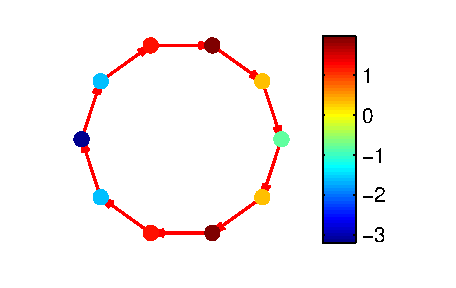
\includegraphics[width=0.40\linewidth]{Figures/d170309_frac_delay_ring_visualization_V5_a.eps}
			}}
	%	\vspace{-0.2cm}
	\subfloat[\label{figb_frac_delay_directed}]{{
			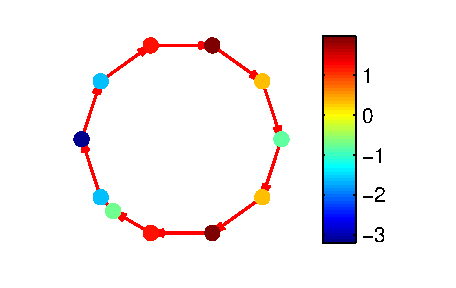
\includegraphics[width=0.40\linewidth]{Figures/d170309_frac_delay_ring_visualization_V5_b.eps}
			}}\\
	\subfloat[\label{figc_frac_delay_directed}]{{
			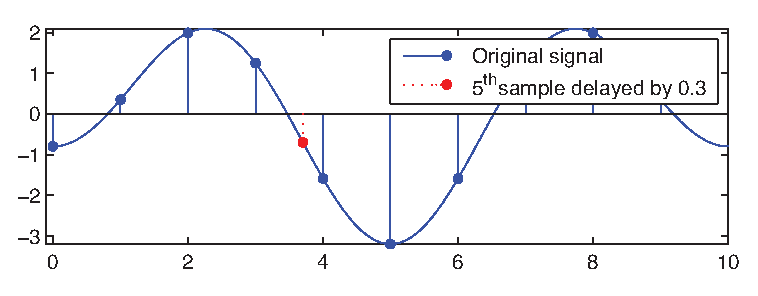
\includegraphics[width=0.85\linewidth]{Figures/d170309_frac_delay_ring_visualization_V5_c1.eps}
			}}% 
	\caption{Fractional shift by $a=0{.}3 $ of a sample of a signal on a directed ring graph with unit weights. (a) Original signal on a directed ring graph. (b) Graph in which the 5$\textsuperscript{th}$ sample delayed by $a=0{.}3 $ appears as an interpolated sample between the 4$\textsuperscript{th}$ and the 5$\textsuperscript{th}$ samples of the original signal. (c) Original discrete signal and the delayed sample.}
	\label{fig:frac_delay_directed}
	%\vspace{-0.3cm}
\end{figure}

\begin{figure*}[h!]
\begin{equation}\label{eq:DFT_inversa_autovalores}
h_a[n]\hspace{-0.03cm}=\hspace{-0.03cm}
\left\{\begin{array}{ll}
%\displaystyle
{\dfrac{1}{N}} \dfrac{\sin (\pi (n-a))}{\sin \left(\frac{\pi}{N} (n-a)\right)}, &\text{ if $N$ is odd},\vspace{0.25cm}\\
%\displaystyle
{\dfrac{1}{N} \cot \left(\dfrac{\pi}{N} (n-a)\right) \sin (\pi (n-a))}{+ \dfrac{j}{N} (-1)^n \sin (\pi a)}, &\text{ if } N \text{ is even}.
\end{array}\right.
\end{equation}
\hrule
\end{figure*}

The product by a fractional power of the adjacency matrix produces the effect illustrated in Fig. \ref{fig:frac_delay_directed}, for a directed ring graph; it can be seen, for example, how the 5\textsuperscript{th} sample of the signal shifted by $a=0{.}3 $ coincides with the value of the continuous-time signal at the same position. On the other hand, the analysis we can perform by observing the \textit{irregular} graph in Fig.~\ref{fig:sinal_Pernambuco} is mostly visual; as we vary the fractional parameter from $0$ (original signal) to $1$, we see in the intermediate snapshots how the signal gradually spreads out from the vertices where, originally, there were already non-zero samples. In this scope, although we employ terms such as delay and shift, which are inherited from classical signal processing, the process observed in the figure looks more like a kind of (fractional) diffusion. In fact, diffusion on graphs have been widely studied~\cite{zhang2008,thanou2017, benzi2021}; it is usually described in terms of a system of ordinary differential equations in time, with the Laplacian matrix of the graph as the coefficient matrix. Fractional diffusion has been used to model certain phenomena that allow long-range interactions and are non-local in nature~\cite{ilic2005,riascos2014,estrada2021,antil2021}. In future works, we intend to investigate the possible relationships between the operator proposed in this paper and the mathematical tools for fractional diffusion in networks. 

Finally, we draw attention to the fact that the signal to be shifted has to be band-limited (see Fig.~\ref{figa_gibbs}). If the signal has abrupt changes in its sample values, this can be viewed as a kind of descontinuity and represents high frequency components, when compared to the predominantly smooth behavior of the signal (see Fig.~\ref{figb_gibbs}). As a consequence, we can observe considerable fluctuations around the disparate samples when the signal is fractionally delayed, an effect similar to the Gibbs phenomenon.

\begin{figure}[t!]
	\centering
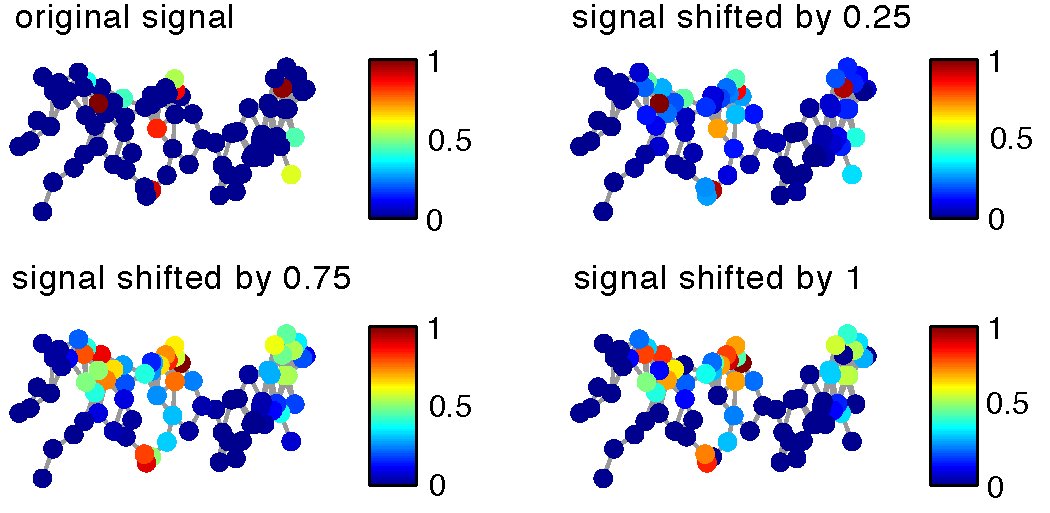
\includegraphics[width=0.95\linewidth]{Figures/signal_PE_V2_PT.pdf}
	\caption{Fractional shift of a signal, (originally) with $10$ non-zero samples, defined on a graph formed by $80$ cities of Pernambuco state, Brazil. Note that the shifted signal is similar to the original signal, if $ a $ is close to $0$, and similar to the unit-shifted signal, if $ a $ is close to $1$.}%
	\label{fig:sinal_Pernambuco}%
	\vspace{-0.2cm}
\end{figure}

\begin{figure}[t!]
	\centering
	\subfloat[\label{figa_gibbs}]{{
			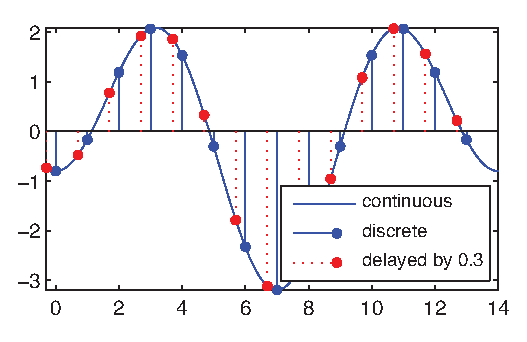
\includegraphics[width=0.8\linewidth]{Figures/d170309_frac_delay_ring_visualization_V2_no_gibbs.eps}
			}}\\
	%	\vspace{-0.2cm}
	\subfloat[\label{figb_gibbs}]{{
			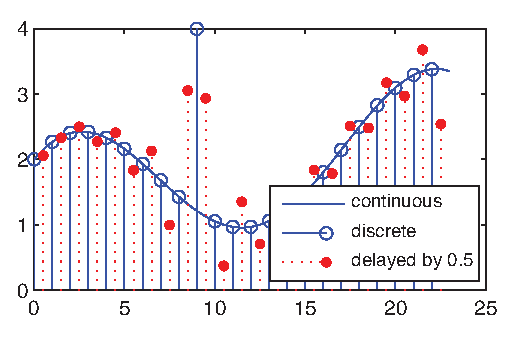
\includegraphics[width=0.78\linewidth]{Figures/frac_delay_ring_TESTS_gibbs_effect.eps}
			}}%
	\caption{Fractional shift for a signal (a) without and (b) with abrupt variations (descontinuities).}%
	\label{fig:frac_delay_gibbs}%
	\vspace{-0.2cm}
\end{figure}

\subsection{Consistency with classical approach: the ideal fractional delay filter}\label{subsec:consist}
In the classical approach to the problem of fractionally shifting a discrete-time signal, the continuous-time version of the signal can be reconstructed by shifting and then resampling with the same sample period~\cite{alan1989discrete,valimaki1995discrete}. Due to the Nyquist-Shannon Theorem, this procedure requires that the signal is band-limited. In this context, it can be shown that, if a discrete-time signal $ \mathbf{x} $ is band-limited, its version shifted by $ a \in [0,1] $ is
$$
x[n-a] = \sum_k x[k] \mathrm{sinc} (n - k - a),
$$
so that the (ideal low-pass) filter used to perform the referred shift has components
\begin{equation}
h_{_{LPF}}[n] = \mathrm{sinc} (n-a).
\end{equation}

The filter $ \mathbf{h}_{_{LPF}} $ is non-causal and unstable (it is not BIBO -- \emph{bounded input, bounded output}, because its impulse response has infinite energy) and, therefore, it is not physically realizable. In this way, fractional delay filter implementations should just \emph{approximate} $ \mathbf{h}_{_{LPF}} $ as much as possible.

In order to evaluate how close to $ h_{_{LPF}}[n] = \mathrm{sinc} (n-a) $, $ 0\leq a \leq 1 $, is $h_a[n]$, for odd $N$ (see the first row of~(\ref{eq:DFT_inversa_autovalores})), the point-wise difference between these signals has been computed for different values of $ N \in [10^1, 10^6]$. In Fig. \ref{fig:convergence}, we show the relative error  (ratio between the energy of the error $(\mathbf{h}_a - \mathbf{h}_{_{LPF}})$ and that of $ \mathbf{h}_{_{LPF}} $), in terms of $ N $ and $a $.

The result suggests that, in fact, $ \mathbf{h}_a $ converges in the mean in $ \ell^2 $ to $ \mathbf{h}_{_{LPF}}$ as $ N $ grows, with relative error less than $ 5\% $ for $ N \approx 30 $. Moreover, the error is greater when $ a $ is close to $ 0{.}5 $, being negligible or null when $ a $ is an integer. In fact, the error is exactly zero for $ a=0$ (or $a=1$) and $ n = a $, since
\begin{equation}\label{eq:lim_h_impar}
\lim_{n \rightarrow a} h_{a}[n] = 1
\Rightarrow
\lim_{n \rightarrow a} \big(h_{a}[n] - \mathrm{sinc}(n-a)\big) = 0.
\end{equation}

The same result is obtained for even $N$, starting from the second row of~(\ref{eq:DFT_inversa_autovalores}). When $a$ is non-integer, $h_a[n] $ is complex, with imaginary part of constant modulus for a fixed $a$. Considering the corresponding real part only, the error was smaller than that taking into account also the contribution of the imaginary part. Fig. \ref{fig:convergence_even_N_real_part} and Fig. \ref{fig:convergence_even_N_abs} show that the errors with and without the imaginary part equally decay as  $ N $ grows, but, using the real part only, the results are significantly better.

\begin{figure}[ht!]
	\centering
	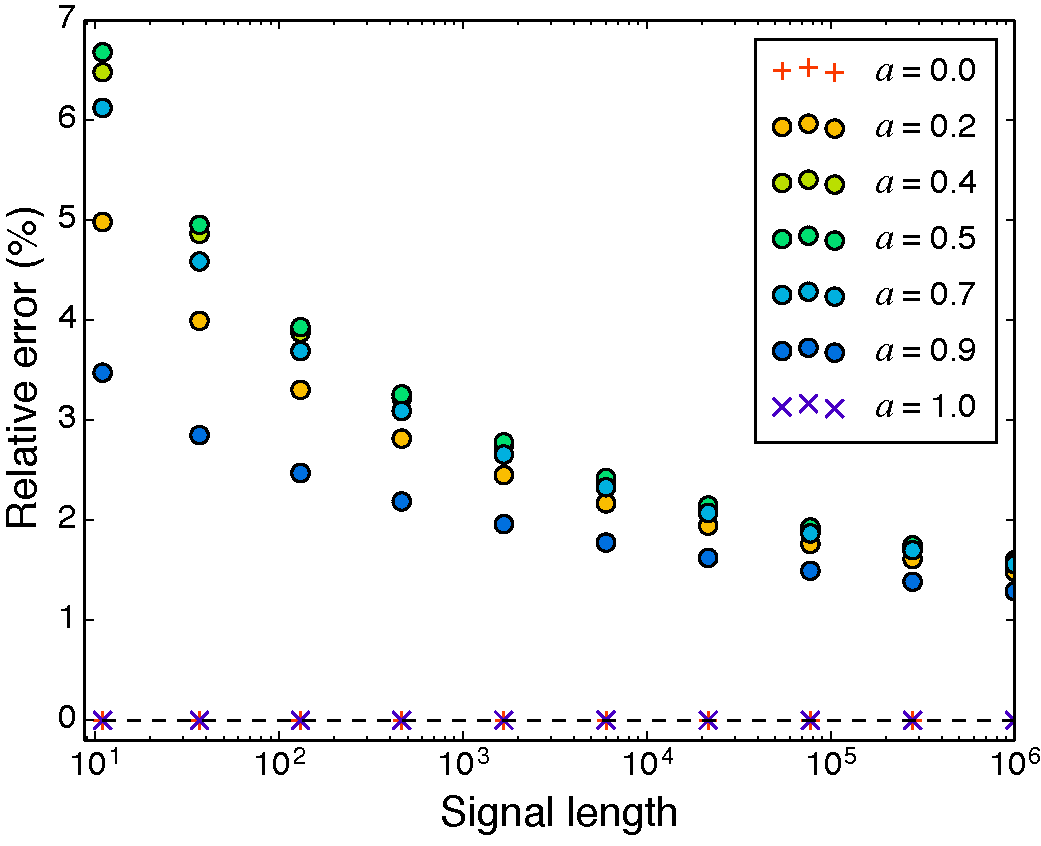
\includegraphics[width=0.81\linewidth]{Figures/convergence_odd_N_V4.pdf}
	\caption{Percent error (normalized by the energy of $ \mathbf{h}_{_{LPF}} $) of $ \mathbf{h}_a $ related to $ \mathbf{h}_{_{LPF}} $, for different (odd) values of $ N $ and the fractional shift parameter $ a $.}
	\label{fig:convergence}
\end{figure}

\begin{figure}[ht!]
	\centering
	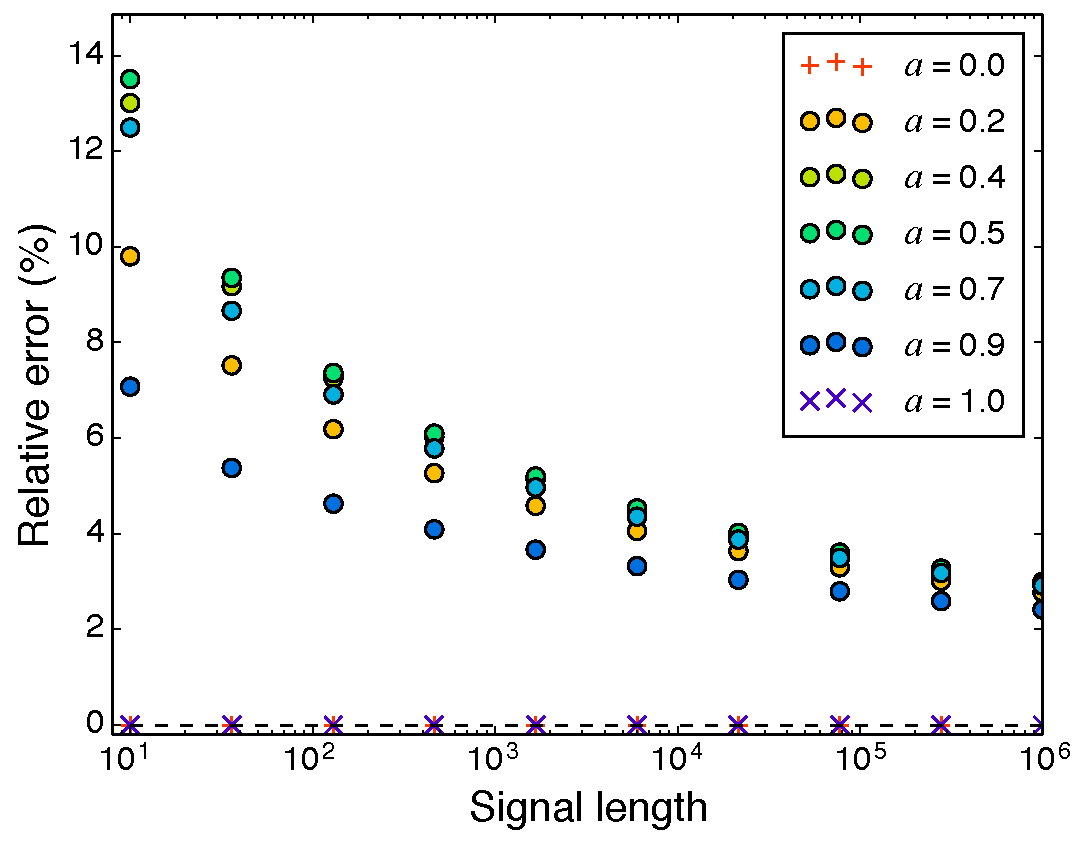
\includegraphics[width=0.81\linewidth]{Figures/convergence_even_N_real_part.pdf}
	\caption{Relative mean error between $ \mathcal{R}e\{\mathbf{h}_a\} $ and $ \mathbf{h}_{_{LPF}} $ for $ N $ even, in terms of the fractional shift parameter $a$.}
	\label{fig:convergence_even_N_real_part}
\end{figure}

\begin{figure}[ht!]
	\centering
	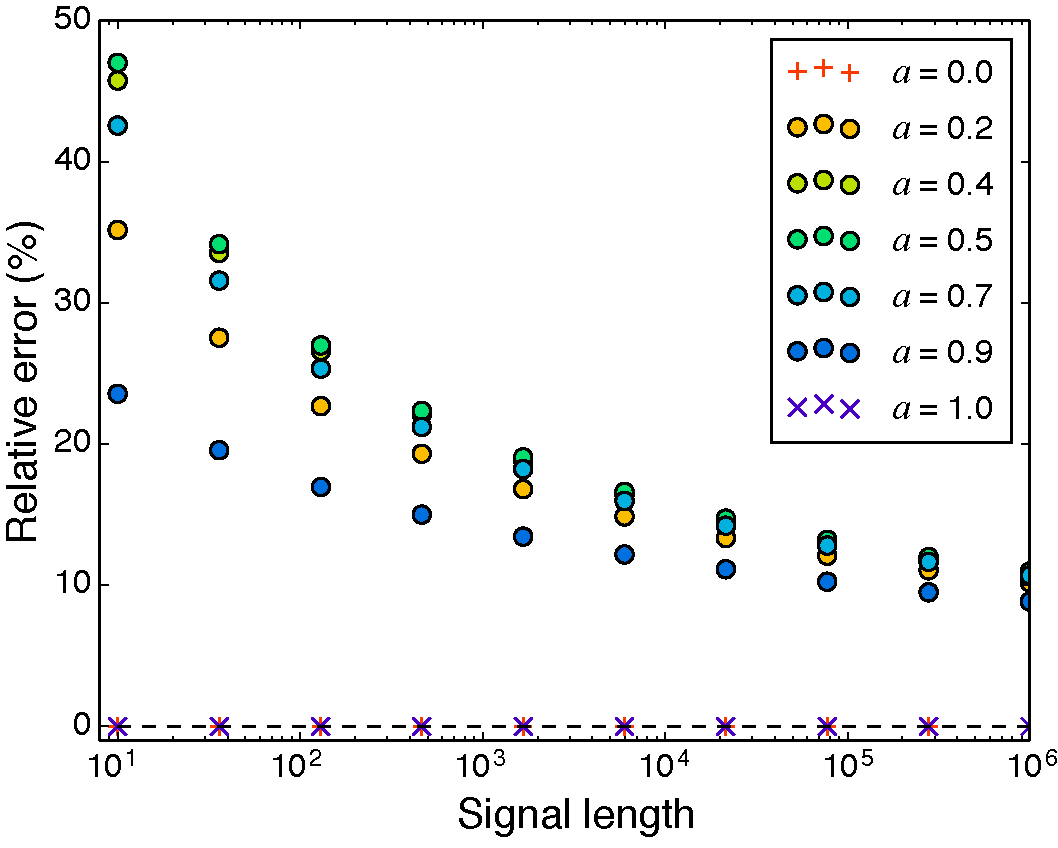
\includegraphics[width=0.81\linewidth]{Figures/convergence_even_N_abs_V2.pdf}
	\caption{Modulus of the relative mean error between $ \mathbf{h}_a $ and $ \mathbf{h}_{_{LPF}} $ for $ N $ even, in terms of the fractional shift parameter $a$.}
	\label{fig:convergence_even_N_abs}
	\vspace{-0.3cm}
\end{figure}

\subsection{Polynomial representation}\label{subsec:poly}
The fractional shift matrix $ \mathbf{A}^a$ necessarily commutes with $ \mathbf{A} $, because $ \mathbf{A}^a\mathbf{A} = \mathbf{A}^{1 + a} = \mathbf{A}\mathbf{A}^a  $, so that $ \mathbf{A}^a $ is an LSI filter for signals on graphs having  $ \mathbf{A} $ as adjacency matrix (see~(\ref{eq:shift_invariance})). Therefore, according to Theorem~\ref{theo:01}, $\mathbf{A}^a$ admits a polynomial representation like the one given in~(\ref{eq:filtro}). In what follows, we evaluate such a possibility for directed ring graphs and for arbitrary graphs.

\vspace{0.25cm}
\noindent\textbf{Directed ring graphs.} The adjacency matrix $ \mathbf{C} $ in~(\ref{eq:C}) of the directed ring graph with unitary weights satisfies $ char_\mathbf{C} = m_\mathbf{C} $ (due to the fact that the eigenvalues of  $\mathbf{C}$ are distinct). Therefore $ \mathbf{H} = \mathbf{C}^a $ can be directly expressed as a polynomial of degree up to  $(N-1)$ in $ \mathbf{C} $. In order to do this, we consider ~(\ref{eq:diag_C}) and the fact that $ \mathbf{F}^{-1} = \mathbf{F}^H $, with $ H $ indicating the conjugate transpose. This allows to show that  $ \mathbf{C}^a = \mathbf{F}^{H} \mathbf{\Lambda}^a_{\mathbf{C}} \mathbf{F}$ is a circulant matrix with the first column given by $ \mathbf{h}_a $ in (\ref{eq:DFT_inversa_autovalores}). Moreover, since the left product of a matrix by $\mathbf{C}$ produces a circular down-shift in each column of the matrix, the $ N $ powers of $\mathbf{C}$ form a basis for the space of $N\times N $ circulant matrices (note that $\mathbf{C}^N =  \mathbf{C}^0$ is the identity matrix). From the above, we conclude that the coefficients of the polynomial representation of $ \mathbf{C}^a $ are the entries of $ \mathbf{h}_a $, i.~e.
\begin{equation}\label{eq:poly_C}
\mathbf{H} = \mathbf{C}^a = \sum_{\ell=0}^{N-1} h_a[\ell] \mathbf{C}^\ell.
\end{equation}

%\subsection{Fun\c{c}\~oes de matrizes}
%
%A teoria de \emph{fun\c{c}\~oes de matrizes} ser\'a aqui utilizada no sentido de mapeamentos $ f: \mathbb{C}^{n \times n}  \rightarrow \mathbb{C}^{n \times n}$ que generalizam, de certa forma, as respectivas fun\c{c}\~oes $ f $ de argumento escalar \cite{higham2008functions}. Pretende-se mostrar a seguir que, utilizando essa teoria, encontra-se para o filtro de deslocamento fracion\'ario proposto uma express\~ao polinomial na matriz de adjac\^encia, de forma que ele \'e LSI. Formalmente, define-se uma fun\c{c}\~ao de matriz como segue \cite{lima2014fractional}.
%
%\begin{definicao}\label{def:01}
%	Seja $ f $ uma fun\c{c}\~ao definida sobre os autovalores de uma matriz $ \mathbf{A} $, de dimens\~ao $ N \times N $, com polin\^omio m\'inimo $ m_{\mathbf{A}}(x) $. Sejam $ \lambda_1, \lambda_2, \dots, \lambda_v $ os autovalores distintos de $ \mathbf{A} $, e $ n_i $ a dimens\~ao do maior bloco de Jordan no qual $ \lambda_i $ aparece. Ent\~ao a fun\c{c}\~ao $ f $ sobre $ \mathbf{A} $ \'e definida como	
%	\begin{equation}\label{eq:matrix_function_01}
%	f(\mathbf{A}) \coloneqq r(\mathbf{A}),
%	\end{equation}
%em que $ r $ \'e o polin\^omio de grau menor que $ \deg m_A $ que satisfaz a interpola\c{c}\~ao
%	\begin{align}\label{eq:matrix_function_02}
%	r^{(j)}(\lambda_i) = f^{(j)}(\lambda_i), \quad
%	&j = 0, 1, \dots, n_i -1 \notag \\
%	&i = 1, 2, \dots, v.
%	\end{align}
%	
%	Se $ n_i = 1 \ \forall i $, $ r $ \'e o polin\^omio interpolador de Lagrange,	
%	\begin{equation}\label{eq:matrix_function_03}
%	r(x) = \sum_{i = 1}^{v} f(\lambda_i) \ell_i (x), \quad
%	\ell_i(x) = \prod_{\substack{k = 1 \\ k \neq i}}^{v} \frac{x - \lambda_k}{\lambda_i - \lambda_k}.
%	\end{equation}
%\end{definicao}
%
%Pode-se mostrar que, para a matriz de adjac\^encia do grafo direcionado em anel com pesos unit\'arios $ \mathbf{C} $, a fun\c{c}\~ao de matriz que generaliza $ f(x) = x^a $, $ 0 \leq a \leq 1 $, \'e
%
%{\color{red} Falta terminar os c\'alculos!}

\noindent\textbf{Arbitrary graphs.} In order to demonstrate how to obtain the polynomial representation of $\mathbf{H}=\mathbf{A}^a$ for arbitrary graphs, we consider another strategy to compute matrix functions. We first remember that, by definition, the minimal polynomial $m_{\mathbf{A}}(t)$ of $\mathbf{A}$ is the unique monic polynomial of lowest degree such that $m_{\mathbf{A}}(\mathbf{A})=\mathbf{0}$. By considering the Jordan canonical form of $\mathbf{A}$, it can be seen that
\begin{equation}
m_{\mathbf{A}}(t)=\prod_{i=1}^s (t-\lambda_i)^{n_i}.
\end{equation}
It follows immediately that $m_{\mathbf{A}}$ is zero on the spectrum of $\mathbf{A}$, that is, the values computed in~(\ref{eq:defspec}) are all zero for $f(t)=m_{\mathbf{A}}(t)$. Given any polynomial $p$ and any matrix $\mathbf{A}\in\mathbb{C}^{N\times N}$, $p$ is clearly defined on the spectrum of $\mathbf{A}$ and $p(\mathbf{A})$ can be defined by substitution. For polynomials $p$ and $q$, $p(\mathbf{A})=q(\mathbf{A})$ if and only if $p$ and $q$ take the same values on the spectrum. Thus the matrix $p(\mathbf{A})$ is completely determined by the values of $p$ on the spectrum of $\mathbf{A}$. The following definition can then be established.
\vspace{0.2cm}
\begin{definition}\label{def:jc02}
Let $f$ be defined on the spectrum of $\mathbf{A}\in\mathbb{C}^{N\times N}$. Then $f(\mathbf{A}):=p(\mathbf{A})$, where $p$ is the unique polynomial of degree less than $\sum_{i=1}^s n_i$ (which is the degree of the minimal polynomial) that satisfies the interpolation conditions
\begin{equation}
    p^{(j)}(\lambda_i)=f^{(j)}(\lambda_i),\quad j=0:n_i-1,\quad i=1:s.
\end{equation}
\end{definition}

The polynomial $p$ above is known as the Hermite interpolating polynomial. In particular, if $n_i=1$, $i=1,\ldots,s$, $p$ corresponds to the Lagrange interpolating polynomial
\begin{equation}
    p(t)=\sum_{i=1}^s f(\lambda_i)l_i(t),\quad l_i(t)=\prod_{j=1,j\neq i}^s \left(\frac{t-\lambda_j}{\lambda_i-\lambda_j}\right).
\end{equation}
In any case, the results briefly presented above lead us to conclude that $\mathbf{A}^a$ can be expressed as a polynomial in $\mathbf{A}$ and, therefore, according to Theorem~\ref{theo:01}, the fractional shift of a graph signal can be implemented as a LSI graph filter.

\section{Numerical Results}\label{sec:num}
In the last section, we have discussed the effect of applying a fractional shift to a graph signal and demonstrated that $\mathbf{A}^a$ admits a polynomial representation. In the first part of this section, we develop a small numerical example to illustrate how the referred representation can be obtained. Secondly, we consider a possibility that, for practical purposes, seems to allow better exploiting the potential for generalization of the proposed fractional operator: replacing $\mathbf{A}$ with $\mathbf{A}^a$ in~(\ref{eq:filtro}) when designing a graph filter. Naturally, the resulting filter, being a polynomial in $\mathbf{A}^a$, could also be expressed as a polynomial in $\mathbf{A}$ and, therefore, it is a LSI filter.

\subsection{Example: Polynomial Representation of $\mathbf{A}^{a}$}\label{subsec:num1}
The graph considered in this example is shown in Fig.~\ref{fig:polyrepres} and has adjacency matrix
\begin{equation}\label{eq:ex001}
%\setlength{\arraycolsep}{3pt}
\mathbf{A}=\left[\begin{array}{ccccc}
5 & 4 & 2 & 1 \\
0 & 1 & -1 & -1\\
-1 & -1 & 3 & 0\\
1 & 1 & -1 & 2
\end{array}\right].
\end{equation}
The entries of $\mathbf{A}$ in~(\ref{eq:ex001}) were chosen so that the Jordan decomposition of such a matrix had integer entries only. The referred decomposition is written using matrices
\begin{equation}\nonumber
%\setlength{\arraycolsep}{3pt}
\mathbf{V}=\left[\begin{array}{ccccc}
-1 & 1&1&1\\
1&-1&0&0\\
0&9&-1&0\\
0&1&1&0
\end{array}\right],\:\:
%\setlength{\arraycolsep}{3pt}
\mathbf{V}^{-1}=\left[\begin{array}{ccccc}
0&1&1&1\\
0&0&1&1\\
0&0&-1&0\\
1&1&1&0
\end{array}\right]
\end{equation}
and
\begin{equation}
%\setlength{\arraycolsep}{3pt}
\mathbf{J}=\left[\begin{array}{ccccc}
1&0&0&0\\
0&2&0&0\\
0&0&4&1\\
0&0&0&4
\end{array}\right].
\end{equation}
Considering $f(t)=t^{0.3}$ and Definition~\ref{def:jc01}, $f(\mathbf{A})=\mathbf{A}^{0.3}$ can be computed according to
\begin{equation}\nonumber
%\setlength{\arraycolsep}{2.5pt}
\mathbf{A}^{0.3}=\mathbf{V}
\left[\begin{array}{ccccc}
f(1)&0&0&0\\
0&f(2)&0&0\\
0&0&f(4)&f'(4)\\
0&0&0&f(4)
\end{array}\right]\mathbf{V}^{-1},
\end{equation}
which gives
\begin{equation}\nonumber
%\setlength{\arraycolsep}{2.5pt}
\mathbf{A}^{0.3}=
\left[\begin{array}{ccccc}
    1.6294  &  0.6294 &   0.3448 &   0.2311\\
         0  &  1.0000 &  -0.2311 &  -0.2311\\
   -0.1137 &  -0.1137  &  1.4020     &    0\\
    0.1137  &  0.1137  & -0.1709  &  1.2311
\end{array}\right].
\end{equation}
The same result can be achieved by using Definition~\ref{def:jc02}, which gives
\begin{align}
    p(\mathbf{A})&=f(\mathbf{A})=\mathbf{A}^{0.3}\nonumber\\
    &=0.6688\mathbf{I}+0.3915\mathbf{A}-0.0654\mathbf{A}^2+0.0051\mathbf{A}^3,\nonumber
\end{align}
the polynomial representation of $\mathbf{A}^{0.3}$.

\begin{figure}
	\centering
	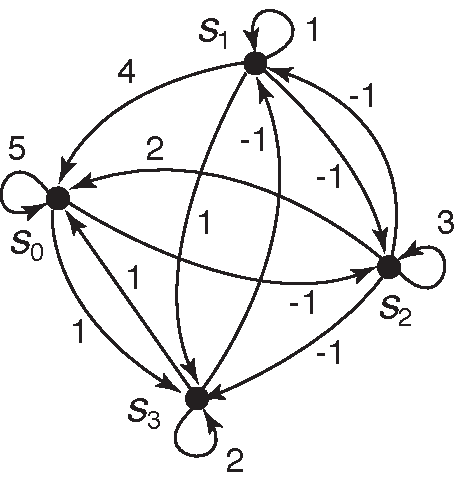
\includegraphics[width=0.55\linewidth]{Figures/graph_jordan.pdf}
	\caption{Directed graph used to illustrate how the corresponding fractional shift operator can be computed and represented in polynomial form.}
	\label{fig:polyrepres}
\end{figure}

\subsection{Least-Square approximation of LSI filters}\label{subsec:lsi}
Before developing a numerical example illustrating the use of $\mathbf{A}^a$ to filter graph signals, we first review a simple design technique that are least-squares approximations of ideal LSI filters~\cite{sandryhaila2014frequency}. Such a method consists of defining the (ideal) filter by specifying the values of $h(\lambda_i)$ (filter response in each eigenvalue of the shift operator), instead of determining the values of $h_{\ell}$ (filter coefficients). Describing the frequency response of the filter for each eigenvalue  $ \lambda_i $, we obtain the linear system of equations
\begin{equation}
\label{eq:siseq}
\begin{aligned}
h(\lambda_0) &= \alpha_0, \\
h(\lambda_1) &= \alpha_1, \\
&\vdots \\
h(\lambda_{N-1}) &= \alpha_{N-1}, \\
\end{aligned}
\end{equation}
or, since $ h(\cdot) $ is a polynomial of degree $ L $,
\begin{equation}\label{eq:syst01}
\begin{aligned}
h_0 + h_1 \lambda_0 + \dots + h_L \lambda^L_0 &= \alpha_0, \\
h_0 + h_1 \lambda_1 + \dots  + h_L \lambda^L_1 &= \alpha_1, \\
&\vdots \\
h_0 + h_1 \lambda_{N-1} + \dots + h_L \lambda^L_{N-1} &= \alpha_{N-1}. \\
\end{aligned}
\end{equation}
Using a Vandermonde matrix constructed from the eigenvalues $\lambda_i$, the system~(\ref{eq:syst01}) can be written in matrix form as
\begin{equation}\label{eq:siseq2}
\setlength{\arraycolsep}{3pt}
\left[\begin{array}{ccccc}
1 & \lambda_0 & \lambda^2_0 & \dots & \lambda^L_0 \\
1 & \lambda_1 & \lambda^2_1 & \dots & \lambda^L_1 \\
& \vdots & & \vdots & \\
1 & \lambda_{N-1} & \lambda^2_{N-1} & \dots & \lambda^L_{N-1} \\
\end{array}\right]
\begin{bmatrix}
h_0 \\
h_1 \\
\vdots \\
h_L
\end{bmatrix} =
\begin{bmatrix}
\alpha_0 \\
\alpha_1 \\
\vdots \\
\alpha_{N-1}
\end{bmatrix}.
\end{equation}
More specifically, if one desires to design a low-pass filter (LPF) whose cutoff frequency is $ \lambda_{i_\text{cut}} $, one could set
\begin{equation}
\label{eq:alfas}
\left\{\begin{array}{ll}
\alpha_i = 1, & \text{for } j = 0,\ldots, i_\text{cut},\\ 
\alpha_i = 0, & \text{for } j = i_\text{cut}+1,\ldots,N-1.
\end{array}\right.
\end{equation}
Since one generally has $ N \geq L+1$, the system of equations~(\ref{eq:siseq2}) is \emph{overdetermined} and does not have an exact solution. A possible strategy is to find coefficients $ h_\ell $, $ \ell=0, \dots, L-1 $, that minimize, in the least-squares sense, the deviation from the ideal filter response. This corresponds to solve the optimization problem
\begin{equation}
\label{eq:opt}
\underset{\{h_\ell\}_{0, \dots, L-1}}{\text{min}} \left( \sum_{n=0}^{N-1} h(\lambda_n) - \alpha_n \right)^2.
\end{equation}

Our proposal is to replace $\mathbf{A}$ with $\mathbf{A}^a$ in~(\ref{eq:filtro}). If this is performed, the only adjustment needed in the technique described above consists of replacing the eigenvalues $\lambda_i$ with their $a^{\text{th}}$ powers $\lambda_i^a$ in~(\ref{eq:syst01}). The effect of such a substitution is illustrated and evaluated in what follows.

\subsection{Example: LS Approximation using $\mathbf{A}^{{a}}$}\label{subsec:lsi01}
In this example, we consider a network formed by $230$ weather stations that measure daily temperature across the United States~\cite{data2011}. Such stations are represented by the vertices of an undirected graph whose edges have been established by using the $8$-nearest neighbor criterion.  The edge connecting vertices $v_n$ and $v_m$ is weighted according with
\begin{equation}
    \mathbf{A}_{n,m}=\frac{e^{-d^2_{n,m}}}{\sqrt{\sum_{k\in\mathcal{N}_n}e^{-d^2_{n,k}}\sum_{\ell\in\mathcal{N}_m}e^{-d^2_{n,\ell}}}},
\end{equation}
where $d_{n,m}$ denotes the geodesical distance between the $n^{\text{th}}$ and the $m^{\text{th}}$ sensors. The snapshot of all measurements taken on February $1^{\text{st}}$, 2003 forms the signal indexed by the referred graph, which is shown in Fig.~\ref{fig:usa00}. From the GFT of the signal, which is plotted in Fig.~\ref{fig:usa01}, it can be seen that its spectral content is concentrated in the low graph frequencies. Note that such frequencies correspond to the eigenvalues of $\mathbf{A}$, which are marked along the horizontal axis of the figure; additionally, the referred marking accompanies the fact that low (resp. high) graph frequencies are associated with higher (resp. lower) eigenvalues~\cite{sandryhaila2014frequency}.

\begin{figure}%
	\centering
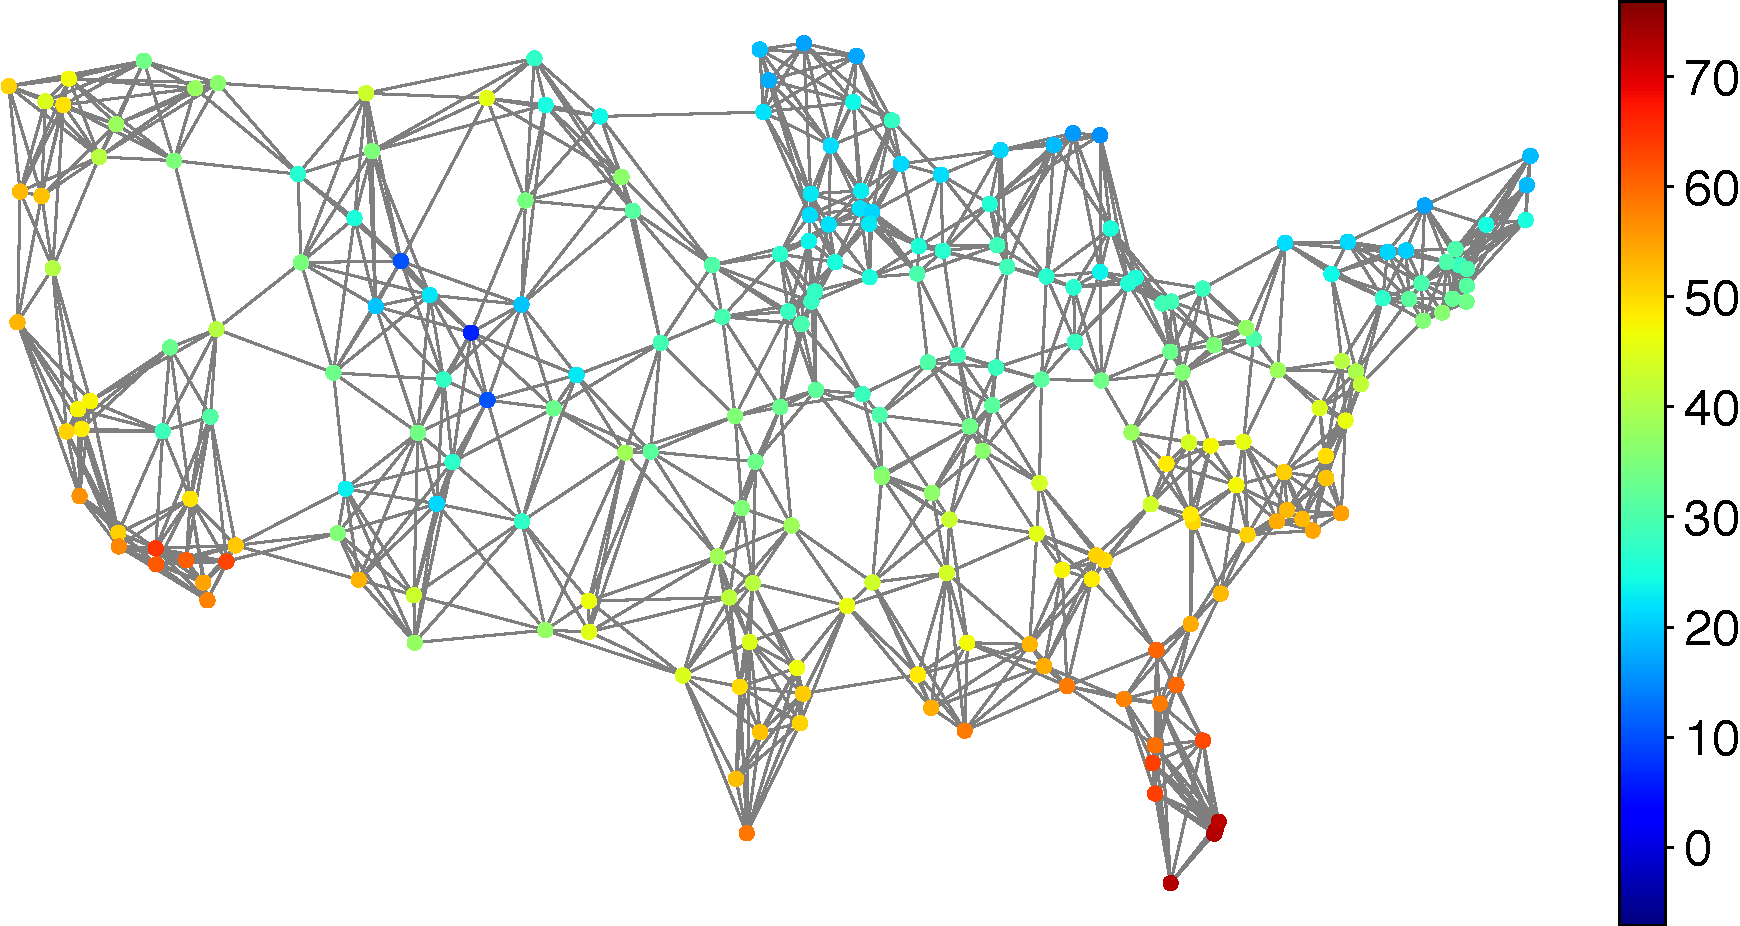
\includegraphics[width=\linewidth]{Figures/GNorm_estacoes_temperatura.pdf}
	\caption{Graph of a network formed by $230$ weather stations measuring the temperature across the United States. The snapshot of all measurements taken on February $1^{\text{st}}$, 2003 is the corresponding graph signal.}%
	\label{fig:usa00}%
	\vspace{0.14cm}
\end{figure}

\begin{figure}[ht!]%
	\centering
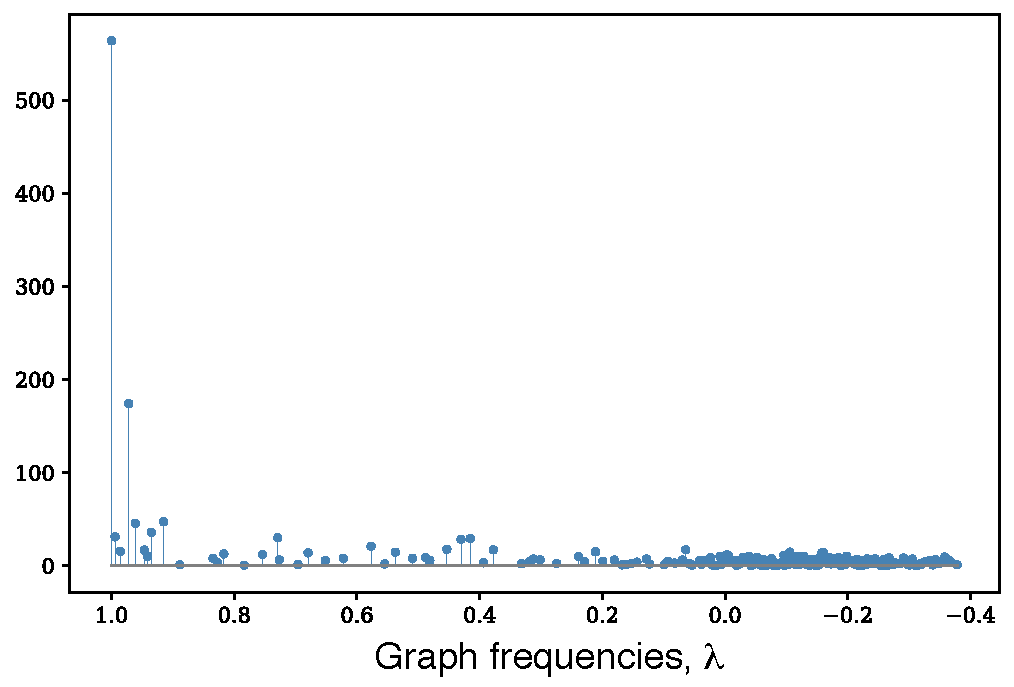
\includegraphics[width=0.88\linewidth]{Figures/GNorm_estacoes_GFT_Temperatura.pdf}%\vspace{-0.1cm}
	\caption{Magnitude of the graph Fourier transform of the signal in Fig~\ref{fig:usa00}. The graph frequencies correspond to the eigenvalues of $\mathbf{A}$; low (resp. high) graph frequencies are associated with higher (resp. lower) eigenvalues.}%
	\label{fig:usa01}%
	%\vspace{-0.2cm}
\end{figure}

\begin{figure}[ht!]
	\centering
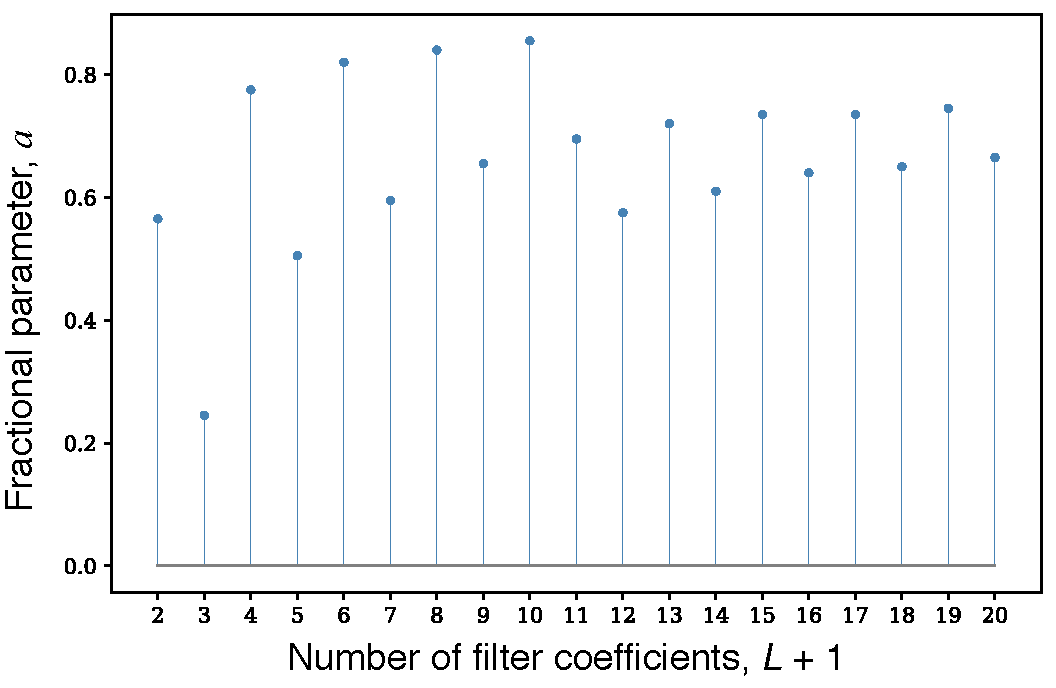
\includegraphics[width=0.9\linewidth]{Figures/ERROR_ordens_fracionarias.pdf}
	\caption{Fractional parameters providing the minimum approximation errors, for different values of $L$, between the ideal LPF and the filter designed by using the fractional graph shift operator $\mathbf{A}^a$.}%
	\label{fig:usa02}%
	%\vspace{-0.5cm}
\end{figure}

We then use the strategy explained in Subsection~\ref{subsec:lsi} to design a filter that approximates an ideal low-pass filter with $\lambda_{i_\text{cut}}=0.2$. In this case, $i_\text{cut}=39$ so that the $40$ lowest graph frequencies are (ideally) preserved after the signal is filtered. We considered approximations with $L$ ranging from $1$ to $19$, that is, filters with $2$ to $20$ coefficients. For each of these values, we varied the fractional parameter $a$ from $0$ to $1$ and, in~(\ref{eq:siseq2}), after replacing $\lambda_i$ with $\lambda_i^a$, $i=0,1,\ldots,N-1$, and solving~(\ref{eq:opt})\footnote{The optimization problem~\ref{eq:opt} has been solved using the Linear Algebra module \emph{linalg} for Scipy, a free and open-source Python library used for scientific and technical computing. In all experiments performed, the least mean squares algorithm converged and the time required for this was negligible, considering the addressed application scenario.}, we registered the value of $a$ providing the minimum error between the designed filter and the ideal filter. At the end of this procedure, the graph shown in Fig.~\ref{fig:usa02} was produced. Observing the figure, we verify that, for any value of $L$, the best approximation is provided when $a\neq1$. This is enough to conclude that, for the graph considered in the example, the use of a fractional version $\mathbf{A}^a$, $a\neq 1$, of $\mathbf{A}$ always provides a better result than the one obtained with the non-fractional matrix. A visual comparison between these alternatives can be performed from Fig.~\ref{fig:usa03}, where we show the (minimum) errors we have just referred to together with the errors when the original (non-fractional) matrix $\mathbf{A}$ is employed.

In Fig.~\ref{fig:usa04}, we can observe the ideal filter response superimposed on the responses obtained when $\mathbf{A}$ and $\mathbf{A}^a$ are used to design a filter with $L+1=10$ coefficients. In this case, the fractional parameter providing the minimum error is $a=0.855$. In the figure, we notice that the filter designed with $\mathbf{A}^a$ has fluctuations that deviate less from the ideal filter, when compared to those related to the filter designed using $\mathbf{A}$. This can be observed mainly in the passband and constitutes a visual result coherent with the obtained approximation errors. Graphs with similar behaviour are obtained for other values $L$.

\begin{figure}[t!]
	\centering
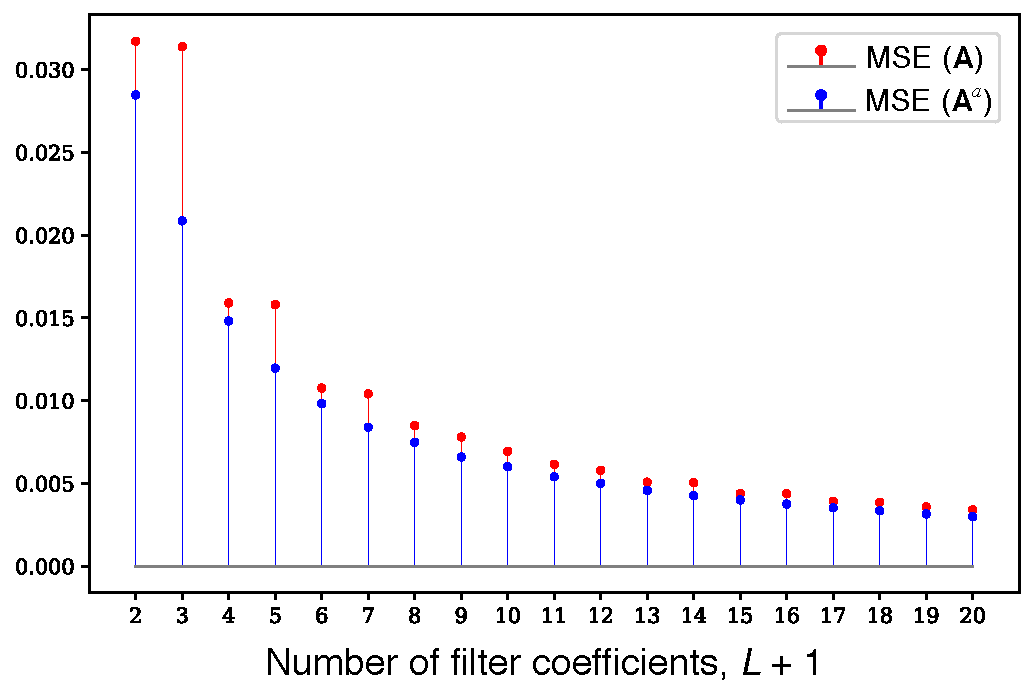
\includegraphics[width=0.9\linewidth]{Figures/ERROR_mse_min.pdf}
	\caption{Minimum approximation (mean squared) errors, for different values of $L$, between the ideal LPF and the filters designed by using the fractional graph shift operator $\mathbf{A}^a$ and the non-fractional operator $\mathbf{A}$.}%
	\label{fig:usa03}%
	%\vspace{-0.2cm}
\end{figure}

\begin{figure}[t!]
	\centering
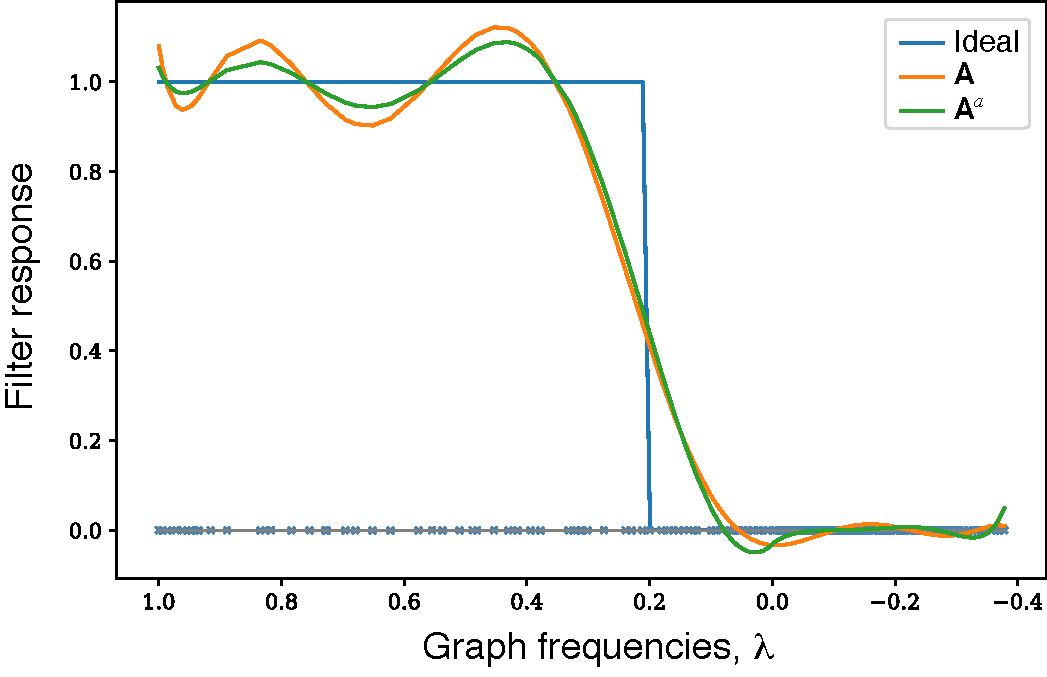
\includegraphics[width=0.88\linewidth]{Figures/ERROR_estacoes_resposta_grau10.pdf}%\vspace{-0.4cm}
	\caption{Ideal filter response superimposed on the responses obtained when $\mathbf{A}$ and $\mathbf{A}^a$, $a=0.855$, are used to design a filter with $L+1=10$ coefficients.}
	\label{fig:usa04}%
	%\vspace{-0.2cm}
\end{figure}

\subsection{Example: Noise Removal}\label{subsec:lsi02}
In this example, we start from the same graph signal considered in Subsection~\ref{subsec:lsi01}. We add to the samples of the referred signal random uniformly-distributed values whose amplitude corresponds to a percentage of the range of the signal itself. Such a synthetic noise addition is intended to simulate what happens in many practical scenarios, in which measurements performed on a sensor network are subject to different sources of distortion. The resulting noisy signal is then filtered by using the filters shown in Fig.~\ref{fig:usa04}, as an attempt to reduce the influence of the noise and recover the original signal.

In our experiment, we varied the aforementioned percentage from $1\%$ to $50\%$ and, for each of these values, we generated $100$ noisy signals. We then filtered such signals and compared the resulting signals with the original (non-noisy) signal by the computation of mean-squared errors. The results, which can be viewed in Fig.~\ref{fig:usa05}, show that the filter designed using $\mathbf{A}^{0.855}$ allows to recover the signal with average reconstruction error always smaller than that related to the filter designed using $\mathbf{A}$. \textcolor{black}{In this context, it is relevant to remark that the (best) fractional parameter $a=0.855$ has been found using the strategy described in the second paragraph of Subsection~\ref{subsec:lsi01}, which depends on the error between the designed filter and the ideal filter only. Therefore, the referred choice does not require us to know the original signal, which is not available in the real-world.} This illustrates the potential gain that can be achieved, in this application scenario, when considering the possibility of fractionalization of the graph shift operator.

\textcolor{black}{Finally, it is also interesting to mention that only one or a few nodes could have had their measurements corrupted by noise or changed due to other factors; this would represent a scenario in which certain sensors would be malfunctioning. In order to obtain some preliminary results taking into account the above described assumption, we carried out additional simulations. To be more specific, we basically repeated our previous tests, but assuming that only a number from $1$ to $12$ nodes had their values nullified or increased by $20$ times. We then performed a low-pass filtering, expecting that the high-frequency component associated with the referred measurement changes would be attenuated and that the smooth behavior of the signal would be recovered. In general, the results obtained using the proposed fractional operator were better or at least equivalent to those obtained with the corresponding ordinary operator. In a future work, we intend to address this issue in more detail.}

\begin{figure}[t!]
	\centering
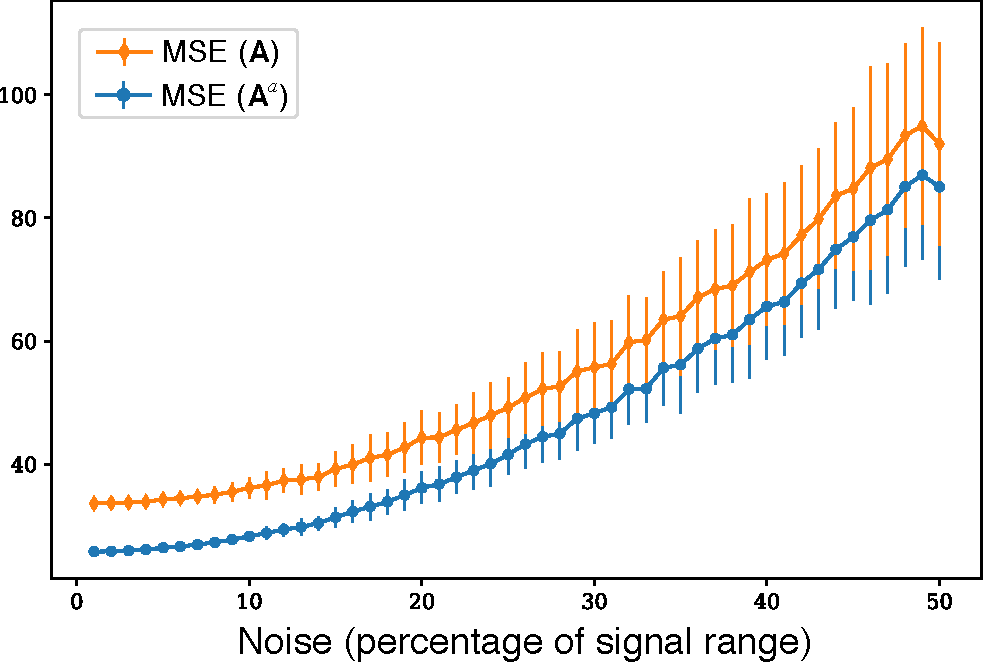
\includegraphics[width=0.95\linewidth]{Figures/ERROR_errobar_filtrados.pdf}
	\caption{Reconstruction (mean squared) errors after a noise removal procedure is performed by using graph filters with $L+1=10$ coefficients and designed from $\mathbf{A}$ and $\mathbf{A}^a$, $a=0.855$.}%
	\label{fig:usa05}%
	\vspace{-0.1cm}
\end{figure}

\section{Concluding Remarks}\label{sec:conc}
In this paper, we have investigated the fractional shift of graph signals. The key-point for our developments is the fact that, in the GSP theory, the unit shift is defined from the adjacency matrix of a graph. Interpreting the fractional shift as a filtering operation, we demonstrated that, for ring graphs, its application produces the expected effect of approximating the classical ideal interpolating filter, exhibiting satisfactory results for band-limited signals. We have also shown that the referred fractional operator can be implemented as an LSI graph filter for arbitrary graphs and developed real-world examples that illustrated the benefits of using $\mathbf{A}^a$ to design graph filters for noise removal. Our current investigations include the study of the fractionalization of other operators on graphs (e.g., graph Fourier transform and Laplacian), other types of generalization for the same operators and further applications of the fractional graph shift. \textcolor{black}{In particular, we have been studying the use of $\mathbf{A}^a$ to design filters for anomaly detection on graphs (malfunctioning nodes in a sensor network, for instance) and evaluating the feasibility of introducing a kind of generalized degree index, so that long range interactions can be considered.}


\chapter{The fractional quaternion discrete Fourier transform and its applications}
\label{ch:FrQDFT}

Linear discrete transforms are building blocks for a multitude of techniques in the field of signal processing, being almost as important as they are diverse. Among the factors which distinguish one from the others, there is the algebraic structure over which they are defined, e.~g. a finite field and its extensions (such as in number-theoretic \cite{blahut2010fast,pedrouzo2017number,chandra2014exact,lima2013} and arithmetic \cite{knockaert1994generalized, rajapaksha2014vlsi} transforms), or the real and complex fields (as in the usual discrete Fourier transform). As the algebra is extended (for instance, from $ \mathbb{R} $ to $ \mathbb{C} $), it is possible to encode more information into each signal sample. Such was the motivation behind Sangwine's definition \cite{sangwine1996fourier} of discrete two-dimensional quaternion transforms, based on their continuous counterparts previously defined by Ell \cite{ell1993quaternion}: to apply these four-dimensional numbers --- the quaternions, an extension of the complex field --- to color image processing. Since then, quaternion transforms have been useful not only to image processing \cite{ell2007hypercomplex,chen2018quaternion,li2013quaternion,evans2000hypercomplex,silva2018}, but also to other fields, such as bivariate signal analysis \cite{flamant2017spectral,flamant2017time,flamant2018complete}.

Fractional transforms are yet another class of tools of great use. The fractional Fourier transform has been applied to time-frequency analysis, compression, digital watermarking, filtering, encryption, let alone its utility in Optics \cite{bultheel2002shattered,figueiredo2018}. Regarding quaternion transforms, a couple of competent works have already addressed their fractionalization \cite{guanlei2008fractional, wei2013different, roopkumar2016quaternionic} and some applications have been proposed \cite{chen2018quaternion}. However, the authors are not aware of papers approaching fractional quaternion discrete transforms from an eigenstructure analysis point of view. This reasoning may unfold new theoretical insights and implementation techniques, and such is the motivation for this work.

In this paper, the eigenstructure of the quaternion discrete Fourier transform (QDFT) matrix is investigated and shown to be closely related to that of the unitary discrete Fourier transform (DFT). This result offers an approach for defining the fractional version of the QDFT (referred to as FrQDFT). Following the central goal of defining the transform through eigendecomposition theory, a generalization is proposed in the form of a multiparametric fractional quaternion discrete Fourier transform (MFrQDFT). For illustrative purposes, this work proposes and briefly explores an encryption scheme for color images with opacity layer, fully harnessing the holistic processing of 4-layered 2D signals through the MFrQDFT.

The proposed method for image encryption fits in the class of schemes that use linear transforms alongside non-linear blocks \cite{hsue2018enhancing}, to implement confusion and diffusion. The currently available methods in the state-of-the-art literature respond to a diverse range of needs, as fast implementation through parallel computing \cite{wang2019fast}, increased safety and robustness by using matrix semi-tensor product \cite{wang2020image} or one-time keys \cite{liu2010}, just to name a few examples. The main scope of this paper is not the encryption scheme \textit{per se}, but rather the FrQDFT eigenscructure and the MFrQDFT definition, the latter having the image encryption as a framework to showcase some of its possibilities. Nevertheless, the proposed encryption algorithm is described and evaluated to some extent. Although being an illustrative scenario, it stands on tools adopted currently by the literature. For example, the chosen method for key generation involved the use of chaotic maps, known to help achieving high bit sensibility and large key space. It follows works such as the one by Liu and Wang \cite{liu2011color}, which proposed a color image encryption scheme using two chaotic maps and one-time keying, aiming to achieve large key space and cycle lengths. Another work by Liu and Wang \cite{liu2012} employed a piecewise linear chaotic map and DNA encoding for ensuring the initial conditions of the encryption change according to the image, whereas Wang \textit{et al.} \cite{wang2010chaotic} used a Lorentz chaotic map and a perceptron model applied to image encryption. The proposed scheme uses a chaotic tent map to generate a pseudo-random sequence, from which the secret parameters are extracted.


This paper is structured as follows. Section \ref{sec:autoestrutura} presents the usual definition of the QDFT and proves the central theorem of this work, regarding how the DFT and QDFT share symmetric eigenvectors; it closes with comments on the quaternion representation of color images with opacity layer. Section \ref{sec:FrQDFT} discusses the fractionalization of the QDFT from an eigenstructure point of view and demonstrates some properties purely based on matrix algebra. Section \ref{sec:multi} proposes a multiparametric extension of the fractional transform and presents an application involving encryption of color images with opacity layer. The main results are summarized in Section \ref{sec:conclusao}, and the paper closes with a brief Appendix on basic quaternion algebra.


\section{Eigenstructure of the QDFT}
\label{sec:autoestrutura}
Quaternion Fourier transforms (QFT) have received quite a few definitions. Some are one-dimensional \cite{flamant2017spectral}, while others are intrinsically two-dimensional \cite{guanlei2008fractional}; the latter group can yet be divided into those having kernels oriented towards generic pure unit quaternions\footnote{The reader may refer to the Appendix to a brief revision on the set of quaternion numbers $ \mathbb{H} $, their algebra and terminology.}, and those using canonic imaginary units, such as $ \qi $ and $ \qj $. The 2D-transformed signals may be placed \textit{between} the two kernels or beside them. In fact, Ell \cite[sec. 3.2]{ell2014quaternion} lists 8 possibilities for the 2D-QFTs.

In this paper, we use the QDFT of axis $ \qmu $ as defined in \cite[sec. 3.3.1]{ell2014quaternion}. Let $ \qmu $ be a unit pure quaternion. Then, the $ m$-th entry of the QDFT of vector $ \mathbf{v} $ is

\begin{equation}
\label{eq:QDFT_fwd}
\!\widehat{v}_m \!=\! \text{QDFT}\{ \mathbf{v} \}_m \!\overset{\Delta}{=}\! \frac{1}{\sqrt{N}} \!\sum_{n=0}^{N-1}  \exp \left( -\qmu \frac{2\pi}{N} nm \right) v_n \!\in\! \mathbb{C}_{\qmu},\!
\end{equation}
in which $ \mathbb{C}_{\qmu} $ denotes the set of numbers $ a + \qmu b $, $ a,b \in \mathbb{R} $, isomorphic to the complex set. It matters to notice that, due to the lack of commutativity in quaternion multiplication, the position of the kernel relative to the signal in (\ref{eq:QDFT_fwd}) is relevant and must be kept consistent along all computations. Hence, the inverse transformation must be computed with the kernel on the same relative position,
\begin{equation}
\label{eq:QDFT_inv}
v_n = \text{QDFT}^{-1}\{ \widehat{\mathbf{v}} \}_n = \frac{1}{\sqrt{N}}\sum_{m=0}^{N-1}  \exp \left( \qmu \frac{2\pi}{N} nm \right) \widehat{v}_m.
\end{equation}

The synthesis and analysis equations may be written in matrix form as
\begin{equation}
\label{eq:QDFT}
\widehat{\mathbf{v}} = \text{QDFT}\{ \mathbf{v} \} = \mathbf{F} \mathbf{v},
\end{equation}
\begin{equation}
\label{eq:QDFT_mtx_inv}
\mathbf{v} = \text{QDFT}^{-1}\{ \widehat{\mathbf{v}} \} = \mathbf{F}^{-1} \widehat{\mathbf{v}},
\end{equation}
where $ \mathbf{F} $ is the unitary QDFT matrix, with entries $ \{\mathbf{F}\}_{n,m} = \sqrt{N}^{-1} \exp \left( -\qmu \frac{2\pi}{N} nm \right)$. Since $ \exp \left( -\qmu \frac{2\pi}{N} \right) $ is an $ N $-th root of unity, such as $ \exp \left( -\qi \frac{2\pi}{N} \right) $, it follows that $ \mathbf{F} $ shares many properties of the DFT matrix, such as invertibility (simple calculations show that $ \mathbf{F}^{-1} = \mathbf{F}^{H} $), what guarantees validity of the inversion formulae in (\ref{eq:QDFT_inv}) and (\ref{eq:QDFT_mtx_inv}).

The two-dimensional QDFT can be defined in a similar fashion, although more options regarding kernel positioning are available, since for any pure quaternions $ \qmu \neq \qnu $, one may verify that generally $ e^{\qnu \alpha} e^{\qmu \beta} \neq e^{\qnu \alpha + \qmu \beta} $. Ell and Sangwine \cite{ell2014quaternion} presented the \textit{eight} distinct ways of building a 2D-QFT, which translate directly into options for 2D-QDFT. One of such possibilities is to transform the quaternion-valued matrix $ \mathbf{X} \in \mathbb{H}^{N\times M}$ according to the equation
\begin{equation}
\label{eq:2DQDFT-01}
\hat{X}_{u,k} = 
\text{2D-QDFT}\{ \mathbf{X} \}_{u,k} \!\overset{\Delta}{=}\! \frac{1}{\sqrt{MN}} \!\sum_{n=0}^{N-1} \sum_{m=0}^{M-1}  \exp \left( -\qmu \frac{2\pi}{N} nu \right) X_{n,m} \exp \left( -\qnu \frac{2\pi}{M} mk \right).
\end{equation}
This formulation of the 2D-QDFT translates into the following matrix equation,
\begin{equation}
\label{eq:2DQDFT-02}
\hat{\mathbf{X}} = \mathbf{F}^{(\qmu)} \mathbf{X} \mathbf{F}^{(\qnu)},
\end{equation}
where the Fourier matrices are similar to the one used in (\ref{eq:QDFT}), except from the pure quaternion which serves as transform axis (shown in the parenthesis). This is a consequence of the \textit{separability} of the 2D-QDFT, by which this transform may be conceived as the successive application of two 1D-QDFTs: once in the rows of $ \mathbf{X} $, once in the columns. Therefore, some results and properties derived for the 1D-QDFT may naturally extend to the two-dimensional case.

Although the quaternion eigenvalue problem has been extensively studied and proven to be challenging \cite{de2002quaternionic,flaut2002eigenvalues,jiang2004algorithm,farid2011eigenvalues}, the investigation of the eigenstructure of matrix $ \mathbf{F} $ may benefit from the similarities between the QDFT and the DFT. As a result of Theorem \ref{th:01}, one is able to deduce the QDFT eigenstructure out of even and odd DFT eigenvectors, by using a variation of Pei's reasoning regarding the 2D-QDFT \cite{pei2010eigenfunctions}.

\begin{theorem}
\label{th:01}
Let $ \mathbf{v} $ be an eigenvector of the unitary DFT with eigenvalue $ \lambda $.
\begin{itemize}
\item[(a)] If $ \mathbf{v} $ has even symmetry (in which case $ \lambda = \pm 1 $), then it is also an eigenvector of the QDFT with eigenvalue $ \lambda $.
\item[(b)] If $ \mathbf{v} $ has odd symmetry (in which case $ \lambda = \pm \qi $), then it is also an eigenvector of the QDFT (of axis, let us say, $ \qmu $) with eigenvalue $ -\lambda \qi \qmu$, i.~e. $ \pm \qmu $.
\end{itemize}
\end{theorem}

\begin{proof}
\begin{itemize}
\item[(a)] If $ \mathbf{v} $ has even symmetry, i.~e. $ v_n = v_{N-n} $ for $ n=1,\dots,N-1 $, then
\begin{equation}
%\label{key}
\sum_{n=0}^{N-1} v_n \sin \frac{2\pi}{N} nm = 0,
\end{equation}
therefore,
\newcommand{\correctinghspace}{-1.8cm}
\begin{equation}
%\small
\label{eq:15}
\begin{aligned}
\sqrt{N} \text{QDFT}\{ \mathbf{v} \}_m &= \sum_{n=0}^{N-1} v_n e^{-\qmu \frac{2\pi}{n} nm} \\
&\hspace{\correctinghspace}
=\sum_{n=0}^{N-1} v_n \left( \cos \frac{2\pi}{n} nm - \qmu \sin \frac{2\pi}{n} nm \right) \\
&\hspace{\correctinghspace}
= \left( \sum_{n=0}^{N-1} v_n \cos \frac{2\pi}{n} nm \right) - \underbrace{\left(  \sum_{n=0}^{N-1} v_n \sin \frac{2\pi}{n} nm \right)}_{=0} \qmu \\
&\hspace{\correctinghspace}
= \left( \sum_{n=0}^{N-1} v_n \cos \frac{2\pi}{n} nm \right) - \underbrace{\left(  \sum_{n=0}^{N-1} v_n \sin \frac{2\pi}{n} nm \right)}_{=0} \qi \\
&\hspace{\correctinghspace}
= \sqrt{N} \text{DFT}\{ \mathbf{v} \}_m = \sqrt{N} \lambda v_m \\
&\hspace{\correctinghspace}
\Rightarrow \text{QDFT}\{ \mathbf{v} \} = \lambda \mathbf{v}.
\end{aligned}
\end{equation}
\item[(b)] If $ \mathbf{v} $ has odd symmetry, i.~e. $ v_n = -v_{N-n} $ for $ n=1,\dots,N-1 $ and $ v_0 = 0 $, then
\begin{equation}
%\label{key}
\sum_{n=0}^{N-1} v_n \cos \frac{2\pi}{N} nm = 0,
\end{equation}
hence,
\begin{equation}
\small
\label{eq:17}
\begin{aligned}
\sqrt{N} \text{QDFT}\{ \mathbf{v} \}_m &= \sum_{n=0}^{N-1} v_n e^{-\qmu \frac{2\pi}{n} nm}\\
&\hspace{\correctinghspace}
=
\sum_{n=0}^{N-1} v_n \left( \cos \frac{2\pi}{n} nm - \qmu \sin \frac{2\pi}{n} nm \right) \\
&\hspace{\correctinghspace}
= {\underbrace{\left( \sum_{n=0}^{N-1} v_n \cos \frac{2\pi}{n} nm \right)}_{=0} - \left(  \sum_{n=0}^{N-1} v_n \sin \frac{2\pi}{n} nm \right) \qmu }\\
&\hspace{\correctinghspace}
= - \left(  \sum_{n=0}^{N-1} v_n \sin \frac{2\pi}{n} nm \right) \qmu.
\end{aligned}
\end{equation}

But, from the odd symmetry assumption,
\begin{equation}
%\label{key}
\begin{aligned}
\sqrt{N}\lambda v_m = \sqrt{N}\text{DFT}\{ \mathbf{v} \}_m &= \sum_{n=0}^{N-1} v_n e^{-\qi \frac{2\pi}{n} nm}= - \left(  \sum_{n=0}^{N-1} v_n \sin \frac{2\pi}{n} nm \right) \qi,
\end{aligned}
\end{equation}
therefore (remember that $ \lambda $ and $ v_m $ commute)
\begin{equation}
\label{eq:19}
\sum_{n=0}^{N-1} v_n \sin \frac{2\pi}{n} nm = \sqrt{N}v_m \lambda \qi.
\end{equation}
From (\ref{eq:17}) and (\ref{eq:19}),
\begin{equation}
\label{eq:20}
\begin{aligned}
\sqrt{N}\text{QDFT}\{ \mathbf{v} \}_m &=  -\sqrt{N}\text{DFT} \{ \mathbf{v} \}_m \qi \qmu \\
&\hspace{\correctinghspace}
= -\sqrt{N}v_m \lambda \qi \qmu \\
&\hspace{\correctinghspace}
\Rightarrow \text{QDFT}\{ \mathbf{v} \} = -\lambda \qi \qmu \mathbf{v}.
\end{aligned}
\end{equation}
\end{itemize}
\end{proof}

The results of Theorem \ref{th:01} are summarized in Table \ref{tab:01}.
This analysis can immediately be extended to the two-dimensional case if one considers the separability of the 2D-QDFT, mentioned after (\ref{eq:2DQDFT-02}). If $ (\mathbf{e}^{(\qmu)}, \lambda_{\qmu}) $ and $ (\mathbf{e}^{(\qnu)}, \lambda_{\qnu}) $ are (column-)eigenvector-eigenvalue pairs of the matrices $ \mathbf{F}^{(\qmu)} $ and $ \mathbf{F}^{(\qnu)} $, respectively, then the 2D signal $ \mathbf{e}^{(\qmu)} \mathbf{e}^{(\qnu)^T}  $ is a 2D-QDFT eigenvector with eigenvalue $ \lambda_{\qmu} \lambda_{\qnu} $ \cite{candan2011}. Therefore, this 2D-QDFT has eight (possibly) distinct eigenvalues: $ \pm 1, \pm \qmu, \pm \qnu, \pm \qmu \qnu $.

\begin{table}[b!]
\center
\captionof{table}{DFT and QDFT eigenvectors.}
\label{tab:01}
\begin{tabular}{ccc}
\toprule
\shortstack{Eigenvector\\ symmetry} & \shortstack{Eigenvalue\\(DFT)} & \shortstack{Eigenvalue\\(QDFT)} \\
\midrule
Even & $ \pm 1 $ & $ \pm 1 $ \\
Odd & $ \pm \qi $ & $ - (\pm \qi) \qi \qmu = \pm \qmu $\\
\bottomrule
\end{tabular}
\end{table}

\subsection{2D-QDFT and color images with opacity layer}
\label{subsec:2D_QDFT}
The 2D-QDFT has been commonly used to process color images, which are represented as matrices of pure quaternions \cite{lu20072d,ell2006hypercomplex,chen2018multiple}. In this representation, each color channel of a certain pixel corresponds to an imaginary component of the pure quaternion. Although this mapping is useful and adequate, it neglects the quaternion scalar part (always set to zero), causing a difference in dimensionality between input and output of the 2D-QDFT: while the image is a 2D signal with three-dimensional components, its spectrum has four-dimensional entries. It surely is not a problem \textit{per se}, rather is an inconvenience, also found when processing real signals with the DFT.

An application free from this inconvenience is the analysis of color images with opacity (or alpha) layer, as in files in PNG format (portable network graphics). In this case, each pixel $ (R,G,B,\alpha) $ is mapped into $ q = \alpha + R \qi + G \qj + B \qk $, forming the quaternion-valued matrix $ \mathbf{X} $. Let us compute the 2D-QDFT by separately transforming the rows and columns using (\ref{eq:2DQDFT-02}), with the same transform axis on both sides,
\begin{equation}
\label{eq:2DQDFT}
\text{2D-QDFT}\{\mathbf{X} \} = \mathbf{F} \mathbf{X} \mathbf{F}^T.
\end{equation}

One should notice that the transformation in (\ref{eq:2DQDFT}) does \textit{not} consist on the successive application of the \textit{same} QDFT to the rows and columns of matrix $ \mathbf{X} $. Due to the noncommutative nature of quaternion multiplication, as it was previously mentioned, different transforms are obtained when choosing between left- or right-multiplications, even though the transform axis is kept unchanged. The operation in (\ref{eq:2DQDFT}) performs a \textit{left} QDFT on the columns and a \textit{right} QDFT on the rows, as it is clear from (\ref{eq:2DQDFT-01}). A 2D-QDFT consisting of the \textit{same} transformation applied in both dimensions must use multiplications with the same orientation, e.~g.
\begin{equation}
\label{eq:2DQDFTv2}
\mathbf{F} \left( \mathbf{F}\mathbf{X}^T \right)^T.
\end{equation}

Fig. \ref{fig:2D_QDFTv1} shows the QDFT -- according to (\ref{eq:2DQDFT}) -- of Fig. \ref{fig:dice}, as another PNG image. As an illustration of the difference in using (\ref{eq:2DQDFT}) or (\ref{eq:2DQDFTv2}), caused by the lack of commutativity in quaternion multiplication, the mean squared error (MSE) between the two spectra was computed. The result was approximately 1070. % Cálculo feito com o script trying_separable_2DQDFT.py


%{\color{red}(Mantemos isso?) \'E curioso observar que, ao processar imagens em PNG utilizando a 2D-QDFT, tanto o sinal (imagem) de entrada como o de sa\'ida s\~ao compostos por quaternions (geralmente) n\~ao-puros, o que permite usar a mesma representa\c c\~ao no dom\'inio do sinal e da transformada. Ao usar a 2D-DFT para processar imagens em escala de cinza, ou a 2D-QDFT para imagens em RGB, o dom\'inio espectral difere daquele do sinal original.}

\begin{figure}
\centering
\subfloat[\label{fig:2D_QDFTv1}]{
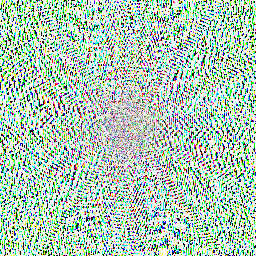
\includegraphics[width=0.3\linewidth]{Figures/2D_QDFTv1.png}
}~
\subfloat[\label{fig:2D_QDFTv2}]{
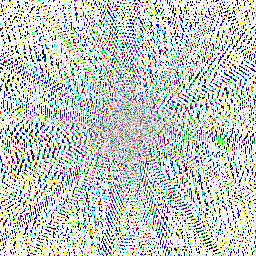
\includegraphics[width=0.3\linewidth]{Figures/2D_QDFTv2.png}
}
\caption{(a) 2D-QDFT of the PNG image in Fig. \ref{fig:dice}, according to (\ref{eq:2DQDFT}), with axis $ \qmu = \frac{1}{\sqrt{3}}(\qi + \qj + \qk) $. (b) 2D-QDFT of the same image, same transform axis, following the approach in (\ref{eq:2DQDFTv2}).}
\label{fig:QDFT}
\end{figure}

\section{Fractional Quaternion Discrete Fourier Transform}
\label{sec:FrQDFT}
%Incluir defini\c{c}\~ao da transformada, a qual sugiro que seja identificada pelo acr\^onimo FrQDFT (do ingl\^es \emph{fractional quaternions discrete Fourier transform}), empregando o conte\'udo desenvolvido na se\c{c}\~ao anterior e abordar as principais propriedades.

The proposed fractionalization method explores the eigenvector sharing between the DFT and the QDFT: as long as one possesses an orthogonal eigenvector matrix $ \mathbf{E} $ for the DFT, it can be used for the QDFT matrix diagonalization and its subsequent fractionalization. For instance, the eigendecomposition of the DFT matrix allows to find its fractional counterpart by raising each eigenvalue to a non-integer parameter $ a $, i.~e.

\begin{equation}
\label{eq:FrDFT}
\mathbf{F}_{\text{DFT}}^a = \mathbf{E} \mathbf{\Lambda}^a \mathbf{E}^T,
\end{equation}
where $ \mathbf{\Lambda} $ is the diagonal matrix containing the DFT eigenvalues.

Oliveira and Lima \cite{de2017discrete} stress that a FrDFT expressed as in (\ref{eq:FrDFT}) will numerically approximate its continuous version if and only if the columns of $ \mathbf{E} $ approximate samples of continuous Hermite-Gaussian functions. In \cite{de2017discrete}, the authors present two methods to generate such an orthogonal eigenbasis, one of which (the generating matrix method) is the one adopted in this work.

\begin{figure*}
\centering
\subfloat[\label{fig:dice}]{
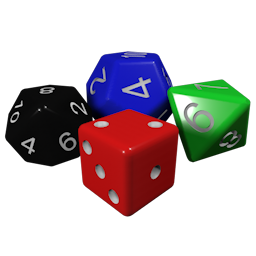
\includegraphics[width=0.25\linewidth]{Figures/dice_256x256.png}
}~
\subfloat[]{
\includegraphics[width=0.35\linewidth]{Figures/dice_256x256_layers.pdf}
}~
\subfloat[]{
\includegraphics[width=0.35\linewidth]{Figures/dice_256x256_layers_frqdft.pdf}
}~
\caption{(a) Test PNG image. Visualization of each layer in the (b) test image and (c) in its FrQDFT spectrum, computed with transform axis $ \qmu = \frac{1}{\sqrt{3}}(\qi + \qj + \qk) $ e $ a=0{.}3 $.}
\end{figure*}

Once one is able to compute an orthogonal eigenbasis $ \mathbf{E} $ containing Hermite-Gaussian-like DFT eigenvectors, for instance by means of the generating matrix method, Theorem \ref{th:01} assures that matrix $ \mathbf{E} $ is also an eigenvector matrix for the QDFT. As a consequence, the transform matrix $ \mathbf{F} $ may be decomposed and written as
\begin{equation}
\label{eq:QDFTmtx}
\mathbf{F} = \mathbf{E} \mathbf{\Gamma} \mathbf{E}^T,
\end{equation}
in which the diagonal matrix $ \mathbf{\Gamma} $ is obtained by replacing $ \qi $ with $ \qmu $ in $ \mathbf{\Lambda} $ (Table \ref{tab:01}). Therefore, the \textit{fractional} quaternion Fourier transform, or simply FrQDFT, is obtained by raising each eigenvalue in $ \mathbf{\Gamma} $ to a so-called fractional order $ a \in \mathbb{R} $, so that
\begin{equation}
\label{eq:QDFTmtxa2}
\text{FrQDFT}_a\{ \mathbf{v} \} \overset{\Delta}{=} \mathbf{F}^a \mathbf{v},
\end{equation}
%\ref{eq:QDFTmtx}
where
\begin{equation}
\label{eq:QDFTmtxa}
\mathbf{F}^a = \mathbf{E} \mathbf{\Gamma}^a \mathbf{E}^T.
\end{equation}

The FrQDFT, as defined in (\ref{eq:QDFTmtxa2}) and (\ref{eq:QDFTmtxa}), possesses all the classical properties of a fractional Fourier transform:

\begin{itemize}
\item \textit{Reduction to the ordinary quaternion transform}: if $ a=1 $, then the synthesis equation in (\ref{eq:QDFTmtxa2}) equals (\ref{eq:QDFT}), coinciding with the QDFT. The proof is imediate.

\item \textit{Reduction to the identity}: if $ a=0 $, the FrQDFT reduces to the identity operator, represented as $ \mathbb{I} $.

\begin{proof}
From the orthogonality of the eigenvector matrix $ \mathbf{E} $,
\begin{equation}
%\label{key}
\mathbf{F}^0 = \mathbf{E} \mathbf{\Gamma}^0 \mathbf{E}^T = \mathbf{E} \mathbf{E}^T = \mathbb{I}.
\end{equation}
\end{proof}

\item \textit{Index addititivy}: applying the FrQDFT twice, using $ a $ and $ b $ as fractional orders, equals applying a single FrQDFT with fractional order $ a+b $. Equivalently, $ \mathbf{F}^a \mathbf{F}^b = \mathbf{F}^{a+b} $.

\begin{proof}
\begin{equation}
%\label{key}
\begin{aligned}
\mathbf{F}^a \mathbf{F}^b &= \mathbf{E} \mathbf{\Gamma}^a \mathbf{E}^T
\mathbf{E} \mathbf{\Gamma}^b \mathbf{E}^T \\
&= \mathbf{E} \mathbf{\Gamma}^a \mathbf{\Gamma}^b \mathbf{E}^T,
\end{aligned}
\end{equation}
but, since $ \mathbf{\Gamma} $ is a diagonal matrix, $ \mathbf{\Gamma}^a \mathbf{\Gamma}^b =
\mathbf{\Gamma}^{a+b} $, hence
\begin{equation}
%\label{key}
\mathbf{F}^a \mathbf{F}^b = \mathbf{E} \mathbf{\Gamma}^a \mathbf{\Gamma}^b \mathbf{E}^T = \mathbf{E} \mathbf{\Gamma}^{a+b} \mathbf{E}^T =
\mathbf{F}^{a+b}.
\end{equation}
\end{proof}

\item \textit{Unitary matrix}: the matrix $ \mathbf{F}^a $ is unitary, i.~e.
\begin{equation}
%\label{key}
\mathbf{F}^a (\mathbf{F}^a)^H = \mathbb{I},
\end{equation}
in which $ (\cdot)^H $ denotes the Hermitian (conjugate transpose) operator.
%\footnote{The \textit{quaternion} conjugation is considered, i.~e. se $ q = a + b\qi + c\qj + d\qk = r \exp (\qmu \theta) $, ent\~ao seu conjugado \'e $ \bar{q} = a - b\qi - c\qj - d\qk = r \exp (-\qmu \theta) $}

\begin{proof}
Since all FrQDFT eigenvalues $ \gamma_n $ are fourth roots of unity in the 1-$\qmu $ plane (i.~e. $ \gamma_n = \pm 1, \pm \qmu $ and, therefore, it has unit module), they can be written as $ \gamma_n = \exp \qmu \theta $ (in which $ \theta = 0, \pm \frac{\pi}{2}, \pi $). Hence
% ent\~ao podem ser escritos na forma $ \gamma_n = \exp \qmu \theta $ (em que $ \theta = 0, \pm \frac{\pi}{2}, \pi $). Assim,
\begin{equation}
%\label{key}
\overline{\gamma^a_n} = \gamma_n = \exp (-a \qmu \theta) = \gamma^{-a}_n,
\end{equation}
consequently
\begin{equation}
\label{eq:24}
(\mathbf{\Gamma}^a)^H = \mathbf{\Gamma}^{-a}.
\end{equation}

From (\ref{eq:24}) and (\ref{eq:QDFTmtxa}),
\begin{equation}
%\label{key}
\begin{aligned}
%\label{key}
(\mathbf{F}^a)^H &=  \left((\mathbf{E} \mathbf{\Gamma}^a) \mathbf{E}^T \right)^H =  \mathbf{E} \left(\mathbf{E} \mathbf{\Gamma}^a  \right)^H =
\mathbf{E} (\mathbf{\Gamma}^{a})^H \mathbf{E}^T = \mathbf{E} \mathbf{\Gamma}^{-a} \mathbf{E}^T = \mathbf{F}^{-a},
\end{aligned}
\end{equation}
and, following the index additivity and the reduction to identity properties,
\begin{equation}
%\label{key}
\begin{aligned}
%\label{key}
\mathbf{F}^a (\mathbf{F}^a)^H = \mathbf{F}^a \mathbf{F}^{-a} = \mathbf{F}^0= \mathbb{I}.
\end{aligned}
\end{equation}
\end{proof}
\end{itemize}

Before proceeding, it matters to notice that other approaches have been used to define fractional transforms, specially suited for image encryption. Lima \textit{et al.} \cite{figueiredo2018} applied the generating matrix method to obtain eigenvectors --- in a fashion similar to this work --- and define multiorder reality-preserving discrete fractional transforms. Roopkumar \cite{roopkumar2016quaternionic}, on the other hand, defined a {continuous} one-dimensional quaternion fractional Fourier transform by using a reasoning similar to the symplectic decomposition of quaternions: adding together two traditional fractional Fourier operators with certain imaginary unit, with one of them multiplied by an orthogonal pure quaternion. None of the approaches, to the best of the authors knowledge, made use of eigenstructure analysis to define the FrQDFT and prove some of its properties.

\section{The multiparametric FrQDFT with Application to Color Image Encryption}
\label{sec:multi}
Frequently, fractional transforms are employed in both grayscale \cite{tao2010image} and color image \cite{kang2018reality, kang2018color} encryption. By setting the secret key to be the transform fractional order, alongside the use of multiple encryption or multiparametric transforms, one is able to create ciphers with sufficiently large key spaces and highly sensible to small key changes. This section presents an illustrative application of the FrQDFT, creating a holistic encryption scheme for PNG images based on the proposition of a multiparametric FrQDFT.

The definition of the multiparametric FrQDFT, referred to as MFrQDFT, consists of employing a different fractional order for each eigenvalue in $ \mathbf{\Gamma} $. The vector of fractional orders is represented by $ \mathbf{a} = [a_0, a_1, \dots, a_{N-1}] $. The MFrQDFT of a column vector $ \mathbf{v} $ is
\begin{equation}
\label{eq:MFrQDFT}
\text{MFrQDFT}\{ \mathbf{v} \} = \mathbf{E} \mathbf{\Gamma^a} \mathbf{E}^T \mathbf{v} = \mathbf{F^a} \mathbf{v}.
\end{equation}

The symbols $ \mathbf{\Gamma^a} $ and $ \mathbf{F^a} $ in (\ref{eq:MFrQDFT}) are abuses of notation. One must comprehend $ \mathbf{\Gamma^a} $ as the diagonal matrix obtained after raising the $ n $-th entry in the diagonal of $ \mathbf{\Gamma} $ to the $ n $-th component in $ \mathbf{a} $. On the other hand, $ \mathbf{F^a} $ indicates the matrix $ \mathbf{E} \mathbf{\Gamma^a} \mathbf{E}^T $. As it was done in Subsection \ref{subsec:2D_QDFT}, the 2D-MFrQDFT of a quaternion matrix $ \mathbf{X} $, e.~g. representing a PNG matrix, is written as
\begin{equation}
\label{eq:2DMFrQDFT}
\text{2D-MFrQDFT}\{\mathbf{X} \} \overset{\Delta}{=} \mathbf{\widehat{X}} = \mathbf{F^a} \mathbf{X} \mathbf{F^a}^T,
\end{equation}
with inverse transform obtained from the properties listed in Section \ref{sec:FrQDFT}
\begin{equation}
\label{eq:2DMFrQDFTinv}
\text{2D-MFrQDFT}^{-1}\{ \mathbf{\widehat{X}} \} = (\mathbf{F^a}^H) \mathbf{\widehat{X}} (\overline{\mathbf{F^a}}).
\end{equation}

\begin{figure*}
\centering
\includegraphics[width=0.9\linewidth]{Figures/esquema_EN.pdf}
\caption{Proposed encryption scheme, exploring the 2D-MFrQDFT.}
\label{fig:cifragem}
\end{figure*}

\begin{figure*}
\centering
\subfloat[\label{fig:ciphered01}]{
\includegraphics[width=0.2\linewidth]{Figures/sage_Encrypted_image.png}
}~
\subfloat[\label{fig:ciphered02}]{
\includegraphics[width=0.25\linewidth]{Figures/Decrypted_image_error_0.png}
}~
\subfloat[\label{fig:ciphered03}]{
\includegraphics[width=0.2\linewidth]{Figures/sage_Decrypted_image_error_minus1dot6.png}
}~
\caption{(a) Encrypted image. (b) Image decrypted with the correct key $ s_0 $. (c) Image decrypted with the wrong key $ \widetilde{s_0} = s_0 + \epsilon $, with $ \epsilon = -1{,}6 \cdot 10^{-80} $.}
\end{figure*}

\subsection{Encryption scheme using MFrQDFT}

The chosen implementation for the PNG image encryption algorithm mixed a block of random-phase modulation (RPM, also called phase mask in \cite{chen2018multiple} and \cite{singh2008optical}) and multiparametric transform. As suggested by \cite{hsue2018enhancing}, a non-linear step of random power is also used. Fig. \ref{fig:cifragem} depicts the system building blocks.

The plaintext image is initially converted into a quaternion matrix $ \mathbf{X} $, which is input to a 2-round processing with RPM $ + $ 2D-MFrQDFT. The random-phase modulation consists of element-wise multiplication by a matrix of random unit quaternions. This role is fulfilled by matrices $ \mathbf{A} $ and $ \mathbf{B} $ in Fig. \ref{fig:cifragem}. The \textit{inverse} RPM (in decryption) is achieved using the \textit{conjugate} of the matrix used during encryption.

The random-power block (RP) is the final step in the encryption method. It creates non-linearity by raising randomly selected entries of the matrix $ \mathbf{X} $ to a random parameter $ \beta \in \ ]0,1[$. This selection is performed by a binary matrix $ \mathbf{R} $, so that the output of the RP block to an input quaternions matrix $ \mathbf{M} $ is
\begin{equation}
%\label{key}
\text{RP}(\mathbf{M})_{i,j} =
\begin{cases}
(\mathbf{M}_{i,j})^\beta & \text{if } \mathbf{R}_{i,j} = 1, \\
\mathbf{M}_{i,j} & \text{if } \mathbf{R}_{i,j} = 0.
\end{cases}
\end{equation}
During decryption, one must use the same matrix $ \mathbf{R} $ and an exponent $ \beta^{-1} $.

A chaotic map was used to generate a pseudorandom sequence $ \mathbf{s} $ of numbers between 0 and 1, from which all of the encryption parameters were drawn: the fractional order vectors $ \mathbf{a} $ and $ \mathbf{b} $ of the two 2D-MFrQDFTs, the parameter $ \beta $ and the matrix $ \mathbf{R} $\footnote{For each entry $ \mathbf{R}_{i,j} $, a corresponding element $ s_k $ of $ \mathbf{s} $ was taken and $ \mathbf{R}_{i,j} $ was set to 1 if and only if $ s_k > 0{,}5 $, $ \mathbf{R}_{i,j} = 0 $ otherwise.} for the RP block. The random-phase modulation matrices were produced beforehand and could be left public in the scheme documentation. The encryption of a $ 256 \times 256 $-pixels image, therefore, requires a sequence of length $ 256 + 256 + 256^2 + 1  $. The secret key consists of the seed $ s_0 $ of the chaotic map, a floating point variable between 0 and 1.
%It is clear how the key space and the scheme security depend on the seed floating-point precision and the chosen chaotic map randomness.
As a consequence, the key space is determined by the smallest deviation $ \epsilon $ from $ s_0 $ so that, using the wrong key $ \widetilde{s_0} = s_0 \pm \epsilon $ in decryption, it still leads to a noisy image without any detectable trace of original information.

The key space dimension, denoted by $ [K] $, is the ratio between the range of all possible keys and the range of wrong keys \textit{which still lead to partial image reconstruction}. The latter is $ [s_0 - \epsilon, s_0 + \epsilon] $, following the previous definition of $ \epsilon $. Since $ s_0 \in \ ]0,1[ $,
\begin{equation}
%\label{key}
[K] = \frac{1 - 0}{s_0 + \epsilon - (s_0 - \epsilon)} = \frac{1}{2 \epsilon}.
\end{equation}

When testing the encryption scheme, the \textit{tent map} \cite{singh2008optical} was chosen as tool for generating the $ \mathbf{s} $ sequence; it is recursively defined as
\begin{equation}
%\label{key}
s_{n+1} =
\begin{cases}
\gamma s_n & \text{if } 0 \leq s_0 < 0{.}5, \\
\gamma(1 - s_n) & \text{if } 0{.}5 \leq s_0 \leq 1.
\end{cases}
\end{equation}
with $0 <  \gamma \leq 2 $.

The tent map parameters were set to $ s_0 = 0{.}3 $ and $ \gamma = 1{.}8 $, for no particular reason other than obeying the range of values for chaotic behaviour. The proposed encryption algorithm was used on the image in Fig. \ref{fig:dice}, what yielded the ciphered output in Fig. \ref{fig:ciphered01}.

In order to evaluate the key space dimension, the ciphered image was decrypted using keys $ \widetilde{s_0} = s_0 \pm \epsilon $ for different values of $ \epsilon \in [-10 \times 10^{-80}; 10 \times 10^{-80}]$, with the aid of multiple precision tools provided by the \textit{RealField} class in the SageMath software. By the end of each decryption, it was computed the MSE between the supposedly recovered image and the original one, what is plotted in Fig. \ref{fig:MSE}. The graph does not change smoothly because each tweak in $ s_0 $ propagates along the whole sequence $ \mathbf{s} $, what affects randomly all the decryption parameters. This is, of course, consequence of the nature of a chaotic map. As shown in the graph, the smallest MSE (still using wrong keys, with $ \epsilon \neq 0 $) was 39dB, obtained with $ \epsilon = -1{,}6 \times 10^{-80} $.

Fig. \ref{fig:ciphered02} and \ref{fig:ciphered03} show the decrypted images using $ \epsilon = 0 $ and $ \epsilon = -1{,}6 \times 10^{-80} $, respectively. It can be seen that the wrong key which caused the smallest MSE still produced a seemingly random PNG image, a desirable property for an encryption scheme. Since the smallest deviation used in this test was $ 0{,}83 \times 10^{-80} $, it follows that the key space dimension is, at least, equal to
\begin{equation}
%\label{key}
[K] = \frac{1}{2 \times 0{,}83 \times 10^{-80}} \approx 6{,}0 \times 10^{79},
\end{equation}
what means the key length must be
%o que significa que cada chave deve ter comprimento de
\begin{equation}
%\label{key}
\lceil 79 \log_2 10 \rceil = 263\text{ bits},
\end{equation}
a value greater than 256 bits, assumed to be appropriate for symmetric encryption schemes, by information security reports such as ECRYPT \cite{smart2018algorithms}. It is also clear from these computations and Fig. \ref{fig:ciphered03} how sensitive the scheme is to small key changes: the smallest modification within the precision of $ 10^{-80} $ in the seed $ s_0 $ was enough to provide a completely noisy decrypted image (cf. Fig. \ref{fig:ciphered03}). The high key sensitivity is also indicated by the sharp dip in the MSE $\times $ Error graph in Fig. \ref{fig:MSE}.
%, \'e um tamanho de chaves apropriado para manter sistemas de cifra sim\'etrica em uso por um per\'iodo estimado de 30 a 50 anos.
%.
%
%%A Fig. \ref{fig:RPM} ilustra a oculta\c c\~ao gradual de informa\c c\~ao visual, ao menos nos pixels n\~ao-nulos, ap\'os cada itera\c c\~ao do bloco de RPM. A cada itera\c c\~ao, uma matriz aleat\'oria diferente \'e usada.
%
\begin{figure}
\centering
\includegraphics[width=10cm]{Figures/MSEdb_FrQDFT_EN.pdf}
\caption{Mean squared error, in dB, between the original and the decrypted images as function of the key error $ \epsilon $.}
\label{fig:MSE}
\end{figure}
%

Such an encryption scheme would not only be safe against brute-force attacks, given its key space dimension, but also known-plaintext attack. The reason for this is the non-linearity provided by the random-power block, as argued intensely by Hsue \cite{hsue2018enhancing}. Resistance to chosen-plaintext attacks, however, is not guaranteed, although simple adjustments could be done in future works to address this problem: the vector of fractional orders $ \mathbf{a} = \{ a_0, a_1, \dots, a_{N-1} \} $ could be made dependent on both the plain image and external parameters (such as the secret seed $ s_0 $). Such tweak in the algorithm would block the extraction of information from comparing chosen plain images with their encrypted counterparts \cite{chai2019color, hu2017chaotic, murugan2016image}, making the scheme resistant to chosen-plaintext and chosen-ciphertext attacks \cite{wang2012novel}; with resistance also to the weaker attacks of brute-force and known-plaintext.

Alongside the investigation of key space dimension and sensitivity, histogram analysis play an important role in describing the performance of encryption schemes. A practical cipher should present an output symbol distribution ideally independent from the cleartext, so that no information is leaked through histogram visualization  \cite{zhang2014symmetric}.
% "An ideal encrypted image should have a
% uniform and completely different histogram against the plain-image for preventing the adversary from extracting any mean-
% ingful information from the fluctuating histogram of the cipher-image." (zhang2014symmetric)
In the case of a PNG image, four histograms are drawn, one for each layer. Fig. \ref{fig:testing_hist} depicts a test PNG image split into its color and opacity components and the corresponding histograms, both prior and after encryption. A group of 13 $ 256\times 256 $-pixels PNG images were encrypted using the proposed method and the histograms of the ciphered output were collected, what is shown in Fig. \ref{fig:allhistograms}. No matter how diverse the input images may be, the histograms present continuously the same profile, what indicates decoupling of information between plain and ciphered images. Although a deeper study on the properties and safety standards of the proposed encryption scheme is needed for full description of its capacity, the analysis presented fit in the scope of this paper and fulfill the goal of presenting the MFrQDFT with a clear and illustrative application.
%{\color{blue}Each image was ciphered using one of the following randomly defined keys (IMPLEMENTAR): $s_0 = $}. % For quantity analyses of each key, we employ variances of histograms to evaluate uniformity of ciphered images. The low-
% er value of variances indicates the higher uniformity of ciphered images. We also calculate the two variances of ciphered
% images which are encrypted by different secret keys on the same plaintext image. The closer of the two values of variances
% indicates the higher uniformity of ciphered images when the secret keys are varying. The variance of histograms is presented
% as follows:

%Histogram analysis: point out that the conversion from float to int, used prior to histogram-making, did not incur in information loss, because the MSE between the original image and the decrypted, AFTER CONVERSION, was
%MSE:  7.380345314385882e-25
%MSEint:  7.380345314385882e-25


\newcommand{\constlength}{0.33}

\begin{figure}[htbp]
\centering
\subfloat[]{\includegraphics[width=0.3\linewidth]{Figures/alphatest_resized_decrypted.png}}~
\subfloat[]{\includegraphics[width=\constlength\linewidth]{Figures/alphatest_resized_decrypted_RGBA_layers.pdf}}~
\subfloat[]{\includegraphics[width=\constlength\linewidth]{Figures/alphatest_resizeddecrypted_histograms.pdf}}\\
\subfloat[]{\includegraphics[width=0.25\linewidth]{Figures/alphatest_resized_encrypted_img.png}}~
\subfloat[]{\includegraphics[width=\constlength\linewidth]{Figures/alphatest_resized_encrypted_RGBA_layers.pdf}}~
\subfloat[]{\includegraphics[width=\constlength\linewidth]{Figures/alphatest_resized_encrypted_histograms.pdf}}
\caption{(a) Test image in PNG format, with 256$ \times $256 pixels. (b) Color and opacity layers of the \textit{decrypted} image (which coincides with the original in (a)). (c) Histograms of each layer of the \textit{decrypted} image. (d) Encrypted image, in PNG format. (e) Color and opacity layers of the \textit{encrypted} image. (f) Histograms of each layer of the \textit{encrypted} image.}
\label{fig:testing_hist}
\end{figure}

\newcommand{\fixedlength}{0.32}
\newcommand{\smallerlength}{0.15}
\begin{figure}[htbp]
\centering
\subfloat[]{\includegraphics[width=\smallerlength\linewidth]{Figures/dice_256x256_decrypted.png}}~
\subfloat[]{\includegraphics[width=\fixedlength\linewidth]{Figures/dice_256x256_encrypted_histograms.pdf}}~
\subfloat[]{\includegraphics[width=\smallerlength\linewidth]{Figures/another_dice_resized_decrypted.png}}~
\subfloat[]{\includegraphics[width=\fixedlength\linewidth]{Figures/another_dice_resized_encrypted_histograms.pdf}}\\
\subfloat[]{\includegraphics[width=\smallerlength\linewidth]{Figures/candle_resized.png}}~
\subfloat[]{\includegraphics[width=\fixedlength\linewidth]{Figures/candle_encrypted_histograms.pdf}}~
\subfloat[]{\includegraphics[width=\smallerlength\linewidth]{Figures/pipe_resized.png}}~
\subfloat[]{\includegraphics[width=\fixedlength\linewidth]{Figures/pipe_encrypted_histograms.pdf}}\\
\subfloat[]{\includegraphics[width=\smallerlength\linewidth]{Figures/dog_resized.png}}~
\subfloat[]{\includegraphics[width=\fixedlength\linewidth]{Figures/dog_encrypted_histograms.pdf}}~
\subfloat[]{\includegraphics[width=\smallerlength\linewidth]{Figures/parrot_resized.png}}~
\subfloat[]{\includegraphics[width=\fixedlength\linewidth]{Figures/parrot_encrypted_histograms.pdf}}\\
\subfloat[]{\includegraphics[width=\smallerlength\linewidth]{Figures/colorparrots_resized.png}}~
\subfloat[]{\includegraphics[width=\fixedlength\linewidth]{Figures/colorparrots_encrypted_histograms.pdf}}~
\subfloat[]{\includegraphics[width=\smallerlength\linewidth]{Figures/bouquet_resized.png}}~
\subfloat[]{\includegraphics[width=\fixedlength\linewidth]{Figures/bouquet_encrypted_histograms.pdf}}
%\caption{Legenda.}
\end{figure}

\stepcounter{figure}
\begin{figure}[htbp]
\centering
\ContinuedFloat
\subfloat[]{\includegraphics[width=\smallerlength\linewidth]{Figures/switzerland_resized.png}}~
\subfloat[]{\includegraphics[width=\fixedlength\linewidth]{Figures/switzerland_encrypted_histograms.pdf}}~
\subfloat[]{\includegraphics[width=\smallerlength\linewidth]{Figures/london_resized.png}}~
\subfloat[]{\includegraphics[width=\fixedlength\linewidth]{Figures/london_encrypted_histograms.pdf}}\\
\subfloat[]{\includegraphics[width=\smallerlength\linewidth]{Figures/russia_resized.png}}~
\subfloat[]{\includegraphics[width=\fixedlength\linewidth]{Figures/russia_encrypted_histograms.pdf}}~
\subfloat[]{\includegraphics[width=\smallerlength\linewidth]{Figures/globe_resized.png}}~
\subfloat[]{\includegraphics[width=\fixedlength\linewidth]{Figures/globe_encrypted_histograms.pdf}}\\
\subfloat[]{\includegraphics[width=\smallerlength\linewidth]{Figures/phones_resized.png}}~
\subfloat[]{\includegraphics[width=\fixedlength\linewidth]{Figures/phones_encrypted_histograms.pdf}}
\caption{Set of 13 PNG test images, 256$ \times $256 pixels, alongside the histograms of each layer (colors and opacity) of their encrypted version. Images downloaded from the online free database \texttt{https://purepng.com/}, under CC0 license.}
\label{fig:allhistograms}
\end{figure}

Finally, as stated at the beginning of the paper, there are a multitude of studies on image encryption, each addressing particular aspects and problems. Therefore, it is adequate to acknowledge the position of this proposed encryption algorithm in the literature landscape. Without providing an extensive and complete analysis, for lack of space, some remarks can be done. The key space dimension in related works vary from circa $ 10^{54} $, around 160 bits, in a work by Wang \textit{et al.} with flexible key space \cite{wang2015novel}, to more than 400 bits, in a paper by Zhang \textit{et al.} \cite{zhang2015new}, an interval which includes the 260 bits of the proposed algorithm. Regarding time of encryption, Wang \textit{et al.} \cite{wang2015novelchaotic} used Arnold cat map and dynamic random growth to obtain large running speed of the encryption and decryption algorithm. This is an aspect our proposed scheme is not optimized for, although great improvement in processing time can be achieved if the eigenvector and eigenvalue matrices of the QDFT are stored in the memory, taking the eigendecomposition out of the encryption process. As a final comment, the main advantages of the scheme proposed in this paper are its modularization, the holistic processing of color images with opacity layer, the lack of long iterations and the ease to describe, comprehend and implement.

\section{Conclusions}
\label{sec:conclusao}
This paper investigated the eigenstructure of the quaternion discrete Fourier transform. Although quaternion matrix decomposition is a challenging topic, the problem for the QDFT was solved by proving that this transform and the DFT share symmetric eigenvectors, what allowed for the construction of an orthogonal eigenbasis of the QDFT, using Hermite--Gaussian-like DFT eigenvectors \cite{de2017discrete}. This result led to the definition of a fractional QDFT, which was proven to hold properties similar to those of the FrDFT, its complex-valued counterpart.

The FrQDFT was further generalized by introducing the MFrQDFT, a multiparametric version. Exploring the 4D nature of quaternions, a holistic encryption scheme for color images with opacity layer was proposed, as an illustrative application of the 2D-MFrQDFT, and shown to provide satisfactorily large key space and key sensitivity, resistance to known-plaintext attack and ease of description and implementation. Future works could possibly expand this analysis and address whether some hypercomplex image moments, such as ternary radial harmonic Fourier moments and quaternion polar harmonic \cite{wang2019ternary,wang2018quaternion}, could be used for image encryption, eventually in specific scenarios and applications.


\chapter{Quaternion graph signal processing}
\label{ch:QGSP}

The application of GSP as a tool to transform graph-based data, as the reader may recall, leaves some characteristics of the underlying graph to be determined by the very problem at hand. That is, whether one must consider real or complex edge weights, directed or undirected graphs, whether loops or multiple edges shall be allowed, all of these modeling choices arise from the data and the relations within. This creates the oportunity to investigate what choices for graph characteristics have so far been left untouched, and what implications they may bring with them.

This Chapter focuses on one of these potential modeling choices. In Chapter \ref{ch:reviewGSP} it was presented the motivation and fundamentals of graph signal processing, while Chapter \ref{ch:FrGSO} delved into the exploration of a fractional graph shift. The following pages will attempt to further extend the borders of GSP by pondering the problem of signal processing on graphs with quaternion-valued edge weights, referred to as \textit{quaternion graph signal processing}.

\red{Pesquisar sobre dados reais que sugiram grafos e sinais quaternionicos?}

\section{Laying the foundations for QGSP}

Since QGSP is the development and application of GSP tools to the context of quaternion-valued signals and graph edge weights, it starts by extending the usual definition of graph signal from the complex-valued case to
\begin{align}\label{eq:qgsp_defs}
\mathcal{G} &= \{\mathcal{V}, \mathbf{A}\}  \ | \ \mathbf{A} \in \mathbb{H}^{n \times n}, \notag \\
s: &\ \mathcal{V} \rightarrow \mathbb{H}^{n \times 1} \ | \ s(v_i) = s_i.
\end{align}
Not surprisingly, writing down the mathematical definitions above is easy enough. The challenges lie in the consequences: what does it mean to have a smooth quaternion graph signal? Does the well known benefit of quaternion signal processing, namely holistic manipulation of multiple channels of information, tranfer to graph signal processing? How is one able to design LSI filters in QGSP?

In order to properly address these questions and establish the foundations of QGSP, a few milestones were set to be conquered:
\begin{itemize}[noitemsep]
\item an algorithm to compute the direct and inverse (quaternion) graph Fourier transforms,
\item a definition of frequency ordering,
\item a method to design filters tailored to certain problems.
\end{itemize}

\subsection{Eigendecomposing the shift operator}
At the very center of vertex-frequency analysis in GSP lies the definition that a basis of eigenvectors of the chosen graph shift operator act as Fourier components for the space of graph signals. This can be directly translated to QGSP, after taking into account the results presented in Chapter \ref{ch:reviewQuat}, regarding diagonalization of quaternion matrices.

\begin{definition}
Given the graph $\mathcal{G} = \{\mathcal{V}, \mathbf{A}\}  $,  with adjacency matrix $ \mathbf{A} \in \mathbb{H}^{n \times n}$, the \textit{quaternion graph Fourier transform} (QGFT) is the projection of a graph signal onto the eigenspace of $\mathbf{A}$.
\end{definition}

The first step to reach the QGFT is, therefore, the generation of a basis of (possibly generalized) eigenvectors of the adjacency matrix. This work has dealt only with the case of diagonalizable graph matrices, but the use of the Jordan canonical form is an option for non-diagonalizable shift operators \cite{Longxuan1996}.

On one hand, from the Corollary \ref{cor:diagonalizable} it is known that the diagonalizability of an adjacency matrix $\mathbf{A}$ both implies and requires that of its complex adjoint matrix $\rchi_A$. Let us write $\mathbf{A} = \mathbf{V} \mathbf{\Lambda} \mathbf{V}^{-1}$. On the other hand, Theorem \ref{th:02} guarantees that the eigenvalues of the adjacency matrix can be taken as half the ones of its complex adjoint matrix. More specifically, they can be taken as the union of the set of eigenvalues with positive imaginary part (recall they are complex-valued) and the set of half the eigenvalues with null imaginary part.

However, once the desired eigenvalues from $\rchi_A$ have been defined, how does one assemble $\mathbf{V}$ out of the eigenvectors of $\rchi_A$? That is answered by Equation (\ref{eq:eigvalueequation}), which is rewritten below for convenience:
\begin{equation*}
\begin{pmatrix}
\mathbf{A}_1 & \mathbf{A}_2\\ 
- \overline{\mathbf{A}}_2 & \overline{\mathbf{A}}_1
\end{pmatrix}
\begin{pmatrix}
\mathbf{v}_1 \\ 
- \overline{\mathbf{v}}_2
\end{pmatrix} =
\begin{pmatrix}
\mathbf{v}_1 \\ 
- \overline{\mathbf{v}}_2
\end{pmatrix}
\lambda.
\end{equation*}
On the left-hand side of the equation, we find $\rchi_A$ and one of its eigenvectors, which is written in terms of the symplectic decomposition of a quaternionic column vector $\mathbf{v} = \mathbf{v}_1 + \mathbf{v}_2 \qj$. As it turns out, $\mathbf{v}$ is precisely the eigenvector of $\mathbf{A}$ associated to the eigenvalue $\lambda$. This is proven in Appendix \ref{ch:AppendixA} and constitutes a minor contribution of this thesis. The answer to the question raised a few lines above, to sum up, is that once one has the chosen eigenvalues of $\rchi_A$, it is possible to assemble $\mathbf{V} \in \mathbb{H}^{n \times n}$ out of the respective eigenvectors of $\rchi_A$ by simply spliting these $2n$-long eigenvectors into two $n$-long halves: the first half corresponds to $\mathbf{v}_1$ (the simplex part of the eigenvector $\mathbf{v}$), while the second half is $- \overline{\mathbf{v}}_2$ (with $\mathbf{v}_2$ being the perplex part of $\mathbf{v}$).

So far we are able to obtain $\mathbf{V}$ from $\mathbf{A}$, using the complex adjoint form to solve the quaternion diagonalization handling only complex-valued matrices. However, the question of how to get $\mathbf{V}^{-1}$, if it exists, poses itself imediately. After all, the direct QGFT must have the shift operator's eigenvectors as \textit{rows} of the transform matrix, since the graph signals are represented as column vectors. Besides, the QGFT must be invertible, so regardless of the representation of graph signals, one must be able to compute the inverse of $\mathbf{V}$. Let us address this point.

\subsection{Inversion of the eigenvector matrix and frequency ordering}
The inversion of quaternion matrices have been tackled by many researchers, yielding a few algorithms aiming at solving it. \red{(INSERT REFERENCES)} All seemed too costly to practical use in medium to large graphs. Based on theorems \ref{th:equiv01} and \ref{th:equiv02},
the algorithm \ref{alg:qinv} is proposed to provide a reasonable balance between processing speed and broad applicability.

The reasoning goes as follows. According to theorem \ref{th:equiv02}, a necessary and sufficient condition for the invertibility of a matrix $\mathbf{V} \in \mathbb{H}^{n \times n}$ is the existance of $\rchi^{-1}_{V}$. Moreover, from theorem \ref{th:equiv01}, if $\rchi^{-1}_{V}$ exists and has the form of a complex adjoint matrix, let us say $\rchi_{V}^{-1} = \rchi_{M}$, then it follows that $\mathbf{M} = \mathbf{V}^{-1}$, since the theorem guarantees that
\begin{equation}
\rchi_{V} \rchi_{M} = \rchi_{V} \rchi_{V}^{-1} = \mathbf{I}_{2n \times 2n} = \rchi_{I_{n \times n}}
\Rightarrow \mathbf{V} \mathbf{M} = \mathbf{I}_{n \times n},
\end{equation}
letting $\mathbf{I}_{m \times m}$ be the identity matrix of order $m$\footnote{For simplicity, this notation is slightly loose, representing both a complex- and a quaternion-valued identity matrix, since in both cases their entries have zero-valued or zero-normed imaginary parts.}.

\newcommand{\algorithmspacing}{0.5}
\begin{algorithm}
\label{alg:qinv}
Compute the inverse of a quaternion-valued matrix, if a sufficient condition for its existence is met:
\vspace*{-\algorithmspacing\baselineskip}
\begin{leftbar}
\noindent\textbf{\upshape Input:} $\mathbf{V} \in \mathbb{H}^{n \times n}$. \textbf{\upshape Output:} $\mathbf{V}^{-1}$ or {\upshape None}.

\begin{algorithmic}[1]
\State $\rchi_V \gets \mathrm{to\_complex\_adjoint}(\mathbf{V})$
\If{$\det(\rchi_V) = 0$} 
    \State \Return {\upshape None}
\Else
    \State $\mathbf{U} \gets \mathrm{inverse}(\rchi_V)$
    \If{$\mathbf{not} \ \mathrm{has\_complex\_adjoint\_form}(\mathbf{U})$}
        \State \Return {\upshape None}
    \Else
        \State $\mathbf{V}^{-1} \gets \mathrm{from\_complex\_adjoint}(\mathbf{U})$
        \State \Return $\mathbf{V}^{-1}$
    \EndIf
\EndIf
\end{algorithmic}
\end{leftbar}
\vspace*{-\algorithmspacing\baselineskip}
\noindent These functions were used in the algorithm to improve readability:
\vspace*{-\algorithmspacing\baselineskip}
\begin{itemize}[noitemsep]
\item $\mathrm{to\_complex\_adjoint}$: converts a quaternion matrix to its complex adjoint form.
\item $\mathrm{from\_complex\_adjoint}$: converts a complex adjoint matrix to its quaternion-valued form.
\item $\mathrm{inverse}$: computes the inverse of a complex-valued matrix.
\item $\mathrm{has\_complex\_adjoint\_form}$: checks if the matrix has the complex adjoint form, i.~e. is a block matrix as the one in Definition \ref{def:complexadjoint}.
\end{itemize}
\end{algorithm}

At this point, all steps required to generate the QGFT, assuming the graph adjacency matrix is diagonalizable, have been addressed. However, the transform still remains of little use until a clear definition of frequency ordering is presented, otherwise the lack of sense of low and high frequencies make the signal spectrum meaningless.

Since the quaternions form a normed algebra --- and the reader may refer back to (\ref{eq:modulusq}) --- it is natural to borrow from classical GSP the definition of the graph total variation as a \textit{metric} for frequency. In fact, even the elegant property of frequency ordering in the complex plane follows from GSP to QGSP. Let us see why.

Let $ \mathbf{A} \in \mathbb{H}^{n \times n}$ be diagonalizable, with standard eigenvalues ordered like so
\begin{equation}
\label{eq:eig_order_q}
|\lambda_0| \leq |\lambda_1| \leq \dots \leq |\lambda_{N-1}| \overset{\Delta}{=} |\lambda_{max}|,
\end{equation}
associated to the eigenvectors $ (\mathbf{v}_i)_{i=0,\dots,n-1} $.
Now, let us notice that the graph total variation, defined in (\ref{eq:tv_graphs}), does not have to use $ \ell_1 $-norm for it to quantify the notion of frequency. In fact, let us use the general $ \ell_p $-norm for a moment, with $p \geq 1$, represented as $ \Vert \mathbf{v}\Vert_p \overset{\Delta}{=} \left(\sum_{k=0}^{n-1} |v_k|^p\right)^{1/p} $, for $\mathbf{v} \in \mathbb{H}^n$, and define the graph total variation of the graph signal $\mathbf{s}$ as
\begin{equation}
\label{eq:tv_graphsq}
TV_{G, p}(\mathbf{s}) \overset{\Delta}{=} \left\Vert \mathbf{s} - \frac{1}{|\lambda_{max}|}\mathbf{A} \mathbf{s} \right\Vert_p.
\end{equation}

If we take the important step of scaling the eigenvectors $\mathbf{v}_i$ so they have unit $\ell_p$-norm, i.~e. making $\Vert \mathbf{v}_i\Vert_p = 1$, then the associative and distributive properties of quaternion multiplication allow us to do

\begin{equation}
\begin{aligned}
TV_{G, p}(\mathbf{v}_k) &=
\left\Vert \mathbf{v}_k - \frac{1}{|\lambda_{max}|} \mathbf{A} \mathbf{v}_k \right\Vert_p =
\left\Vert\mathbf{v}_k - \mathbf{v}_k \frac{1}{|\lambda_{max}|} \lambda_k \right\Vert_p \\
&= \left\Vert\mathbf{v}_k \left( 1 -  \frac{1}{|\lambda_{max}|} \lambda_k \right) \right\Vert_p \\
&=
\underbrace{\Vert \mathbf{v}_k \Vert_p}_{= 1} \left|1 - \frac{\lambda_k}{|\lambda_{max}|}\right| = \Big| \lambda_k - |\lambda_{max}| \Big| \frac{1}{|\lambda_{max}|}.
\end{aligned}
\end{equation}
% Since $(1 -  \nicefrac{1}{|\lambda_{max}|} \lambda_k)$ is just a constant complex factor that multiplies each entry in the vector $\mathbf{v}_k$, its modulus may be taken out of the sum in the $\ell_p$-norm computation,
What leads to exactly the same frequency ordering obtained in the classical GSP derivation,
\begin{equation}
\label{eq:TV_ordering_q}
\Big| \! \lambda_i  - \! |\lambda_{max}|\Big| \! \leq \! \Big|  \lambda_j  - \! |\lambda_{max}|\Big| \! \! \iff \! \! TV_{G, p}(\mathbf{v}_i) \leq TV_{G, p}(\mathbf{v}_j).
\end{equation}

In other words, once the eigenvectors are individually \textit{normalized}, i.~e. scaled to have unit $\ell_p$-norm, then the farther an eigenvalue lies from the point $|\lambda_{max}|$ in the real line of the complex plane, the greater is its eigenvector graph total variation $TV_{G, p}$. By definition, it means the greater is the frequency it represents. Besides, notice how the scaling implies that the value of $TV_{G, p}$ depends solely on the eigenvalues, not on $p$.

In order to interpret the spectrum domain, the eigenvalues are sorted in ascending order of their respective eigenvector total variation: this sorts the frequency from lowest to highest. When not explicitly mentioned, it is assumed a value of $p = 1$ for all occurrences of $\ell_p$-norm.

\subsection{On the existence of a class of graphs with diagonalizable adjacency matrix}

A relevant topic of discussion, when laying the foundations for QGSP, is to ponder the question on the existence of a class of graphs with diagonalizable shift operators. It is a reasonable point of investigation, since in classical GSP one can confidently take advantage of some classes of graphs to make sure the shift operator is diagonalizable beforehand, which saves time and effort. Some examples are undirected real-weighted graphs and directed ring graphs with equal edge weights.

The reader may notice that undirected quaternion graphs do not possess necessarily a diagonalizable adjacency matrix. Indeed, the fact that $\mathbf{A}$ is symmetric has no effect of proving the diagonalizability of its complex adjoint,
\begin{equation}
\begin{pmatrix}
\mathbf{A}_1 & \mathbf{A}_2\\ 
- \overline{\mathbf{A}}_2 & \overline{\mathbf{A}}_1
\end{pmatrix}.
\end{equation}

The subjacent reason as to why undirected real-weighted graphs have diagonalizable adjacency matrices is that these real-valued matrices are symmetric, or more generally \textit{normal}, i.~e. they commute with (because are equal to) their transpose. In the case of complex-valued matrices, being normal (i.~e. commuting with their Hermitian transpose) also suffices for proving their diagonalizability. So, in order to find quaternion graphs analogous to undirected real-weighted graphs, in the sense of having a sufficient condition for diagonalizable shift operators, their adjacency matrix must possess \textit{normal} complex adjoint matrices. Fortunately, Theorem \ref{th:equiv01} states the condition:
 $ \rchi_{A}$ is normal ($ \rchi_{A}^H \rchi_{A} = \rchi_{A} \rchi_{A}^H $) or Hermitian ($\rchi_{A}^H = \rchi_{A}$) if and only if so is $ \mathbf{A}$.
 
 Zhang claims the proof of Theorem \ref{th:equiv01} is by direct verification, but let us go through a way to visualize part of the proof within the context of GSP.
 
\begin{proof}
The part of the Theorem about to be verified is: \emph{is it true that Hermitian quaternion-valued matrices have Hermitian complex adjoints?} Equivalently,
\begin{equation}
\mathbf{A}^H = \mathbf{A}, \ \mathbf{A} \in \mathbb{H}^{n \times n} \Rightarrow
\rchi_{A}^H = \rchi_{A}, \ \rchi_{A} \in \mathbb{C}^{2n \times 2n}?
\end{equation}
\end{proof}

\subsection{Does a Hermitian QGSO have unitary eigenvector matrix?}

It is known that every Hermitian complex matrix is diagonalizable by a unitary matrix. In other words, if $\mathbf{M} \in \mathbb{C}^{n \times n}$ and $\mathbf{M} = \mathbf{M}^H$, then there exists a complex matrix $\mathbf{U}$ and a diagonal matrix $\mathbf{\Gamma}$ so that $\mathbf{M} = \mathbf{U} \mathbf{\Gamma} \mathbf{U}^{-1}$ and $\mathbf{U}^{-1} = \mathbf{U}^H$. However, despite the fact one can guarantee that a Hermitian QGSO has a Hermitian complex adjoint matrix, \textit{it is not true that its eigenvector matrix is necessarily unitary}.

Let $\mathbf{A}$ be a Hermitian (hence diagonalizable) quaternion adjacency matrix, therefore $\mathbf{A} \mathbf{V} = \mathbf{V} \mathbf{\Lambda}$. Since $\rchi_{A}$ is complex-valued and Hermitian, its eigenvector matrix (let us say, $\mathbf{\Phi}$) is unitary and we may write $\rchi_{A} = \mathbf{\Phi} \mathbf{\Gamma} \mathbf{\Phi}^H$. Each column $\mathbf{\qphi}$ in $\mathbf{\Phi}$, the reader may recall, is written is terms of the simplex and perplex parts (which are complex-valued) of the respective column $\mathbf{v}$ in $\mathbf{V}$:
\begin{equation}
\mathbf{\qphi}^{(n)} = 
\begin{pmatrix}
\mathbf{v}^{(n)}_1 \\ 
- \overline{\mathbf{v}}^{(n)}_2
\end{pmatrix}.
\end{equation}

Since $\mathbf{\Phi}$ is unitary,
\begin{equation}
\label{eq:phi_hermitian}
\begin{aligned}
{\mathbf{\qphi}^{(n)}}^H \mathbf{\qphi}^{(n)} = 1 \\
\Big({\mathbf{v}^{(n)}_1}^H \quad - {\mathbf{v}^{(n)}_2}^T \Big)
\begin{pmatrix}
\mathbf{v}^{(n)}_1 \\ 
- \overline{\mathbf{v}}^{(n)}_2
\end{pmatrix} = 1 \\
{\mathbf{v}^{(n)}_1}^H \mathbf{v}^{(n)}_1 + {\mathbf{v}^{(n)}_2}^T \overline{\mathbf{v}}^{(n)}_2 = 1.
\end{aligned}
\end{equation}

Now, does the final equality in (\ref{eq:phi_hermitian}) imply that ${\mathbf{v}^{(n)}}^H \mathbf{v}^{(n)} = 1$? If so, this would make the quaternion-valued eigenvector matrix $\mathbf{V}$ unitary. Let us drop the superscript $n$ temporarily, to clean the notation during the following lines. Since $\mathbf{v} = \mathbf{v}_1 + \mathbf{v}_2 \qj$,
\begin{equation}
\begin{aligned}
\mathbf{v}^H \mathbf{v} &= (\mathbf{v}^H_1 - \mathbf{v}^T_2 \qj) (\mathbf{v}_1 + \mathbf{v}_2 \qj) \\
&= \mathbf{v}^H_1 \mathbf{v}_1 + \mathbf{v}^H_1 \mathbf{v}_2 \qj
- \underbrace{\mathbf{v}^T_2 \qj \mathbf{v}_1}_{\mathbf{v}^T_2 \overline{\mathbf{v}}_1 \qj} - \underbrace{\mathbf{v}_2^T \qj \mathbf{v}_2 \qj}_{- \mathbf{v}_2^T \overline{\mathbf{v}}_2} \\
&= \underbrace{\mathbf{v}_1^H \mathbf{v}_1 + \mathbf{v}_2^T \overline{\mathbf{v}}_2}_{= 1} +
(\mathbf{v}^H_1 \mathbf{v}_2 - \mathbf{v}_2^T \overline{\mathbf{v}}_1) \qj \\
&= 1 + (\mathbf{v}^H_1 \mathbf{v}_2 - \mathbf{v}_2^T \overline{\mathbf{v}}_1) \qj.
\end{aligned}
\end{equation}

That is, unless the complex adjoint eigenvector $\mathbf{\qphi}^{(n)} = \big( \mathbf{v}^{(n)}_1 \quad - \overline{\mathbf{v}}^{(n)}_2 \big)^T$ satisfies the additional constraint ${\mathbf{v}^{(n)}}^H_1 {\mathbf{v}^{(n)}}_2 - {\mathbf{v}^{(n)}}_2^T {\overline{\mathbf{v}}^{(n)}}_1 = 0$, a Hermitian QGSO \textit{does not have} a unitary eigenvector matrix. As a practical consequence, the inverse eigenvector matrix cannot be computed simply by taking its complex conjugate, and an invertibility test must be performed before trying to compute the QGFT matrix.

% In fact, the eigenvector matrix may even be degenerate, as the following example demonstrates.
\red{(But I have not found a single counterexample! Is the additional constraint always met?)}

\subsection{Numerical example: computing the QGFT matrix}

Let the graph in Figure \ref{fig:degenerate_qgft_graph} have the following adjacency matrix,
\begin{equation}
\small
\mathbf{A} = \begin{pmatrix}
0 & 0 & 0 & 1 -7\qi -5\qj -1\qk & 6 +3\qi +7\qj +4\qk \\
0 & 0 & 0 & 0 & 6 +9\qi +2\qj +6\qk \\
0 & 0 & 0 & 0 & 7 +4\qi +3\qj +7\qk \\
1 +7\qi +5\qj +1\qk & 0 & 0 & 0 & 7 +2\qi +5\qj +4\qk \\
6 -3\qi -7\qj -4\qk & 6 -9\qi -2\qj -6\qk & 7 -4\qi -3\qj -7\qk & 7 -2\qi -5\qj -4\qk & 0 \\
\end{pmatrix}.
\end{equation}

As expected, since $ \mathbf{A}$ is Hermitian, so it is its complex adjoint:
\begin{equation}
\small
\rchi_A = 
\begin{pmatrix}
0 &  0 &  0 &  1 -7 \qi &  6 +3 \qi &  0 &  0 & 0 & -5 -1 \qi &  7 +4 \qi \\
0 &  0 &  0 &  0 &  6 +9 \qi &  0 &  0 & 0 &  0 &  2 +6 \qi \\
0 &  0 &  0 &  0 &  7 +4 \qi &  0 &  0 & 0 &  0 &  3 +7 \qi \\
1 +7 \qi &  0 &  0 &  0 &  7 +2 \qi &  5 +1 \qi &  0 & 0 &  0 &  5 +4 \qi \\
6 -3 \qi &  6 -9 \qi &  7 -4 \qi &  7 -2 \qi &  0 & -7 -4 \qi & -2 -6 \qi & -3 -7 \qi & -5 -4 \qi &  0 \\
0 & 0 & 0 &  5 -1 \qi & -7 +4 \qi &  0 &  0 & 0 &  1 +7 \qi &  6 -3 \qi \\
0 & 0 & 0 & 0 & -2 +6 \qi &  0 &  0 & 0 &  0 &  6 -9 \qi \\
0 & 0 & 0 & 0 & -3 +7 \qi &  0 &  0 & 0 &  0 &  7 -4 \qi \\
-5 +1 \qi & 0 & 0 & 0 & -5 +4 \qi &  1 -7 \qi &  0 & 0 &  0 &  7 -2 \qi \\
7 -4 \qi &  2 -6 \qi &  3 -7 \qi &  5 -4 \qi & 0 &  6 +3 \qi &  6 +9 \qi & 7 +4 \qi &  7 +2 \qi &  0
\end{pmatrix}.
\end{equation}

Since the matrix $\rchi_A$ is complex-valued and Hermitian, it is diagonalizable by a unitary matrix $\mathbf{\Phi}$. The eigenvalues of $\rchi_A$ are all real-valued and appear in pairs:
\begin{equation}
\mathrm{diag}(\mathbf{\Gamma}) = \begin{pmatrix}
-22.83570384 \\
-22.83570384 \\
-6.34920255 \\
-6.34920255 \\
0 \\
0 \\
6.45799327 \\
6.45799327 \\
22.72691312 \\
22.72691312 \\
\end{pmatrix}.
\end{equation}
The next step is to take half the eigenvalues of $\rchi_A$ (the ones with positive imaginary part, plus half the real-valued ones) to obtain the standard eigenvalues of $\mathbf{A}$ and the respective eigenvectors. It is important to take one eigenvalue for each pair, to avoid picking eigenvectors from the same eigenspace. Therefore, $\mathrm{diag}(\mathbf{A}) = (-22.83570384, -6.34920255, 0, 6.45799327, 22.72691312)^T$.

\begin{landscape}
The chosen eigenvalues will determine the eigenvectors of $\rchi_A$ used to assemble those from $\mathbf{A}$. The resulting eigenvector matrix (with rounded rounded, to fit the page) is
\begin{equation*}
\footnotesize
\mathbf{V} = \left(\begin{matrix}
-0.24  -0.27\qj +0.16\qk & 0.59  -0.02\qj +0.04\qk & 0  & -0.02  -0.52\qj -0.28\qk & -0.040  +0.38\qj +0.03\qk \\
-0.17 -0.19\qi -0.22\qj +0.17\qk & -0.31 +0.13\qi +0.09\qj +0.16\qk & -0.410 +0.24\qi +0.39\qj -0.23\qk  & -0.05 +0.01\qi -0.12\qj +0.35\qk & -0.010 +0.05\qi +0.20\qj +0.31\qk \\
-0.25 -0.12\qi -0.11\qj +0.13\qk & -0.21 +0.14\qi +0.20\qj +0.09\qk & 0.190 -0.40\qi -0.48\qj +0.37\qk  & -0.1 -0.04\qi +0.01\qj +0.31\qk & 0.010 -0.05\qi +0.26\qj +0.21\qk \\
-0.26 +0.01\qi +0.04\qj +0.25\qk & -0.25 -0.48\qi -0.25\qj -0.06\qk & 0  & 0.36 -0.13\qi +0.30\qj -0.36\qk & -0.110 -0.03\qi +0.27\qj +0.21\qk \\
0.31 +0.18\qi -0.25\qj -0.52\qk & -0.02 -0.15\qi -0.07\qj -0.09\qk & 0  & 0.07 -0.04\qi +0.10\qj +0.14\qk & 0.380 +0.14\qi +0.55\qj +0.04\qk \\
\end{matrix}\right)
\end{equation*}

This matrix passes the inversibility test, since its determinant is $\mathrm{det}(\mathbf{V}) = \mathrm{det}(\rchi_V) = 1 \neq 0$. Not only that, the matrix is also unitary, since the product $\mathbf{V} \mathbf{V}^H$ yields an identity matrix. Therefore, the QGFT matrix is promptly determined.

Figure \ref{fig:simple_example_tv} closes the example, depicting the graph total variation for each normalized eigenvector. The values of $TV_{G, p}$ are \textit{(2, 1.2780384 , 1, 0.71719754, 0.00476406)}, and remain the same as $p$ is changed, following the commentary after (\ref{eq:TV_ordering_q}).

\begin{figure}
\centering
\includegraphics[width=0.35\linewidth]{thesis/Figures/simple_example_tv.pdf}
\caption{Graph total variation of the normalized eigenvectors, as a function of their respective eigenvalues.}
\label{fig:simple_example_tv}
\end{figure}

\end{landscape}

\begin{figure}
\centering
\includegraphics[width=0.3\linewidth]{thesis/Figures/degenerate_qgft_graph.pdf}
\caption{Graph used in the numerical example. The edges are represented by double-headed arrows to indicate the adjacency matrix is not symmetrical.}
\label{fig:degenerate_qgft_graph}
\end{figure}


% \section{A more general sufficient condition}
% A promising thread may be found, however, in the work \textit{Block diagonalization and eigenvalues}, by Eisenfeld \cite{eisenfeld1976block}, from which the following theorem is taken.

% \begin{theorem}[Theorem 3.2 \cite{eisenfeld1976block}]
% Let $\mathbf{M}$ be the $n \times n$ complex-valued block matrix
% \begin{equation}
% \begin{pmatrix}
% \mathbf{E} & \mathbf{F}\\ 
% \mathbf{G} & \mathbf{H}
% \end{pmatrix},
% \end{equation}
% with entries defined on a generic algebra $\mathcal{A}$ and $\mathbf{E}$ and $\mathbf{H}$ having respective orders $p \times p$ and $q \times q$, $p + q = n$.

% Now let $\mathbf{R}_1$ be a solution to the equation
% \begin{equation}
% \mathbf{R} (\mathbf{E} + \mathbf{F} \mathbf{R}) =
% \mathbf{G} + \mathbf{H} \mathbf{R},
% \end{equation}
% and let $\mathbf{X}$ be a root of the linear equation,
% \begin{equation}
% (\mathbf{E} + \mathbf{F} \mathbf{R}_1) \mathbf{X} - \mathbf{X} (\mathbf{H} - \mathbf{R}_1 \mathbf{F}) = - \mathbf{F}.
% \end{equation}
% Then,
% \begin{equation}
% \mathbf{M} = \mathbf{W}
% \begin{pmatrix}
% \mathbf{E} + \mathbf{F} \mathbf{R}_1 & \mathbf{0}_{pq}\\ 
% \mathbf{0}_{qp} & \mathbf{H} -  \mathbf{R}_1 \mathbf{F}
% \end{pmatrix}, \qquad
% \mathbf{W} = 
% \begin{pmatrix}
% \mathbf{I}_p & \mathbf{X}\\ 
% \mathbf{R}_{1} & \mathbf{R}_{1} \mathbf{X} + \mathbf{I}_{q}.
% \end{pmatrix}
% \end{equation}
% \end{theorem}

% \red{(n\~ao consegui muita evolu\c c\~ao daqui. Ignorar resto da subse\c c\~ao.)}
% \begin{equation}
% \begin{aligned}
% R (A_1 + A_2 R) = - \bar{A_2} + \bar{A_1} R \\
% R (A_1 - \bar{A_1}) + R^2 A_2 + \bar{A_2} = 0.
% \end{aligned}
% \end{equation}
% Let us slice the space of possible solutions $R$, restricting ourselves to the case where $A_1 + A_2 R = 0$:
% \begin{equation}
% \begin{aligned}
% - \bar{A_2} + \bar{A_1} R = 0 \\
% R = \bar{A_1}^{-1} \bar{A_2}
% \end{aligned}
% \end{equation}

% Now let $X$ be a solution to the equation:
% \begin{equation}
% \begin{aligned}
% (A_1 + A_2 R)X - X(\bar{A_1} - R A_2) = - A_2 \\
% (A_1 + A_2 \bar{A_1}^{-1} \bar{A_2})X - X(\bar{A_1} - \bar{A_1}^{-1} \bar{A_2} A_2) = - A_2
% \end{aligned}
% \end{equation}

\section{Filter design via QLMS optimization}
\red{Explain here how we performed filter design using QLMS.}

\section{Examples}

This section is devoted to experimenting with QGSP in real-world datasets, tackling topics such as graph inference, spectral analysis, compression and denoising. All computations in this chapter were performed using \texttt{gspx}, an open-source Python package dedicated to implement the core concepts and tools of QGSP. It constitutes a contribution of this thesis and is available at \url{https://github.com/gboaviagem/gspx}.

\subsection{Denoising a quaternion graph signal via QLMS low-pass filtering}

Let us walk through an example on spectral analysis with real-world data using QGSP. The graph signal will be generated using UK towns' weather data, specifically humidity, atmospheric pressure, temperature and wind speed. The data was fetched from the Open Weather Map API\footnote{The API is accessible, as of August 2022, at the address \url{https://home.openweathermap.org/}.}, in April 20th 2022, at approximately 13:00 GMT. The latitude and longitude values of UK towns originate from the LatLong.Net database\footnote{Accessible, as of August 2022, at the address \url{https://www.latlong.net/category/towns-235-55.html}.}.

\begin{figure}
	\centering
	\includegraphics[width=0.3\linewidth]{thesis/Figures/uk_qgsp_graph.pdf}
	\caption{Graph created using the towns in England.}
	\label{fig:uk_graph}
\end{figure}

The graph was created using a nearest-neighbors approach, as in (\ref{eq:weights}), since the nodes possess a clear relation to geographic location. The edge weights were defined using the following steps:
\begin{itemize}[noitemsep]
\item Compute a real-valued nearest-neighbors adjacency matrix based on the latitude and longitude of UK towns (graph nodes), using the ten closest neighbors to each graph node. At this point, the real-valued edge weights correspond to the euclidian distances between nearby towns \textit{i} and \textit{j}, represented by ${d}(i, j)$.
\item For each pair of connected nodes from the real-weighted graph in the previous step, compute the \textbf{absolute difference} in \textit{humidity}, \textit{temperature} and \textit{wind speed}, represented respectively by ${h}(i, j)$, ${t}(i, j)$ and ${w}(i, j)$.
\item For each pair of connected nodes, create the quaternion $q(i, j) = {d}(i, j) + \qi {h}(i, j) + \qj {t}(i, j) + \qk {w}(i, j)$ and set as edge weight the value
\begin{equation}
% \label{eq:}
\mathbf{A}_{i, j} = \exp^{-1} \left(\frac{q}{\theta} \right).
\end{equation}
For the current example, it was chosen $\theta = 0.5$.
\end{itemize}
Figure \ref{fig:uk_graph} depicts a representation of the UK Town Graph, with quaternion-valued edge weights. A total of 177 towns were used, and the reader may find the full dataset at \url{https://github.com/gboaviagem/gspx/blob/main/resources/uk_weather_at_20Apr202213pm.gz}. The first few rows, so it becomes clear how the data is organized, are displayed in Table \ref{tab:02}.

\begin{table}
\center
\captionof{table}{Sample of the dataset containing UK towns' weather data \red{Update!}}
\label{tab:02}
\begin{tabular*}{\textwidth}{c @{\extracolsep{\fill}} cccc}
\toprule
& \textbf{town} & \textbf{latitude} & \textbf{longitude} & \textbf{humidity (\%)} \\
\midrule
1 & Troon, Scotland & 55.540001 & -4.66 & 55\\
2 & St.Asaph, Wales & 53.257999 & -3.442 & 59\\
3 & Stirling, Scotland & 56.1166 & -3.9369 & 53\\
4 & Welling, Bexley, London & 51.4566 & 0.1056 & 39 \\
5 & Bonnybridge, Scotland & 56.003227 & -3.888634 & 50\\
\midrule
\end{tabular*}
\begin{tabular*}{\textwidth}{c @{\extracolsep{\fill}} cccc}
& \textbf{pressure (hPa)} & \textbf{temp (K)} & \textbf{wind speed (m/s)} & \textbf{wind degrees} \\
\midrule
1 & 1018 & 289.19 & 3.6 & 220 \\
2 & 1017 & 288.49 & 3.71 & 99 \\
3 & 1018 & 288.15 & 3.72 & 114 \\
4 & 1014 & 290.09 & 8.23 & 80 \\
5 & 1018 & 288.0 & 3.53 & 106 \\
\bottomrule
\end{tabular*}
\end{table}

% With the quaternion-valued adjacency matrix $\mathbf{A}$ at hand, it was verified that this quaternion graph shift operator (QGSO) was diagonalizable and the direct ($\mathbf{V}^{-1}$) and inverse ($\mathbf{V}$) QGFT matrices were computed. Figure \ref{fig:uk_graph_tv} shows the total variation of the eigenvectors associated with the adjacency matrix eigenvalues.

% \begin{figure}
% 	\centering
% 	\includegraphics[width=0.6\linewidth]{thesis/Figures/uk_qgsp_sig.pdf}
% 	\caption{Each component of the quaternion graph signal.}
% 	% \label{fig:graph_tv_1}
% \end{figure}

% \begin{figure}
% 	\centering
% 	\includegraphics[width=0.6\linewidth]{thesis/Figures/uk_qgsp_tv1.pdf}
% 	\caption{Eigenvalues of the quaternion graph adjacency matrix, shown in the complex plane. The pseudo-colorscale indicates the respective eigenvectors total variation.}
% 	\label{fig:graph_tv_1}
% \end{figure}

% \begin{figure}
% 	\centering
% 	\includegraphics[width=0.6\linewidth]{thesis/Figures/uk_qgsp_spectrumsig_norm1.pdf}
% 	\caption{Eigenvalues of the quaternion graph adjacency matrix, shown in the complex plane. The pseudo-colorscale indicates the respective eigenvectors total variation.}
% 	% \label{fig:graph_tv_1}
% \end{figure}

% \begin{figure}
% 	\centering
% 	\includegraphics[width=0.6\linewidth]{thesis/Figures/uk_ss1_abs.pdf}
% 	\caption{Eigenvalues of the quaternion graph adjacency matrix, shown in the complex plane. The pseudo-colorscale indicates the respective eigenvectors total variation.}
% 	% \label{fig:graph_tv_1}
% \end{figure}

% \begin{figure}
% 	\centering
% 	\includegraphics[width=0.6\linewidth]{thesis/Figures/uk_qgsp_tv2.pdf}
% 	\caption{Eigenvalues of the quaternion graph adjacency matrix, shown in the complex plane. The pseudo-colorscale indicates the respective eigenvectors total variation.}
% 	\label{fig:graph_tv_2}
% \end{figure}

% \begin{figure}
% 	\centering
% 	\includegraphics[width=0.6\linewidth]{thesis/Figures/uk_qgsp_spectrumsig_norm2.pdf}
% 	\caption{Eigenvalues of the quaternion graph adjacency matrix, shown in the complex plane. The pseudo-colorscale indicates the respective eigenvectors total variation.}
% 	% \label{fig:graph_tv_1}
% \end{figure}

% \begin{figure}
% 	\centering
% 	\includegraphics[width=0.6\linewidth]{thesis/Figures/uk_ss2_abs.pdf}
% 	\caption{Eigenvalues of the quaternion graph adjacency matrix, shown in the complex plane. The pseudo-colorscale indicates the respective eigenvectors total variation.}
% 	% \label{fig:graph_tv_1}
% \end{figure}

One may define a quaternion graph signal as being composed by the four last columns of weather data in UK towns (see Table \ref{tab:02}). That is, each sample corresponds to the quaternion with components $(1, \qi, \qj, \qk)$ respectively equal to humidity, pressure, temperature and wind speed in the given town. The scale disparity between components is removed by scaling each column to be within range $[0, 1]$. A way of visualizing the graph signal is to plot each quaternion dimension separately, as done in Figure \ref{fig:uk_qgsp_graphsig}.

\begin{figure}
	\centering
	\includegraphics[width=0.5\linewidth]{thesis/Figures/uk_signal.pdf}
	\caption{Quaternion graph signal, visualized in the vertex domain. The panels (a) to (d) depict, respectively, the real, $\qi$, $\qj$ and $\qk$ components of each quaternion-valued sample.}
	\label{fig:uk_qgsp_graphsig}
\end{figure}

\red{Rewrite this paragraph. Comment on the eigenvectors total variation, in Figure \ref{fig:uk_qgft_tv1}} Complementary to the vertex-domain visualization is the spectrum of the signal. This is obtained by the direct QGFT,
\begin{equation}
% \label{}
\widehat{\mathbf{s}} = \mathbf{V}^{-1} \mathbf{s},
\end{equation}
and the signal frequency components are shown in Figure \ref{fig:uk_qgsp_spectrumsig}.

\begin{figure}
	\centering
	\includegraphics[width=0.7\linewidth]{thesis/Figures/uk_qgft_tv1.pdf}
	\caption{Graph eigenvectors total variation using $\ell_1$-norm.}
	\label{fig:uk_qgft_tv1}
\end{figure}

\begin{figure}
	\centering
	\includegraphics[width=0.7\linewidth]{thesis/Figures/uk_qgft_spectrumsig.pdf}
	\caption{Spectrum of the graph signal in the symmetric graph.}
	\label{fig:uk_qgsp_spectrumsig}
\end{figure}


\begin{figure}
	\centering
	\includegraphics[width=0.7\linewidth]{thesis/Figures/cost_vs_iterations.pdf}
	\caption{.}
	\label{fig:cost_vs_iterations}
\end{figure}

\begin{figure}
	\centering
	\includegraphics[width=0.7\linewidth]{thesis/Figures/qlms_filter.pdf}
	\caption{.}
	\label{fig:qlms_filter}
\end{figure}

\begin{figure}
	\centering
	\includegraphics[width=0.7\linewidth]{thesis/Figures/ideal_filter_output.pdf}
	\caption{.}
	\label{fig:ideal_filter_output}
\end{figure}

\begin{figure}
	\centering
	\includegraphics[width=0.7\linewidth]{thesis/Figures/qlms_filter_output.pdf}
	\caption{.}
	\label{fig:qlms_filter_output}
\end{figure}

\subsubsection{Comparison between signal smoothness in symmetric and Hermitian graphs}
\red{Draw a comment here about the drawback of using Hermitian graphs (which we know have always diagonalizable adjacency matrices): they do not capture the expected relation between signal samples when the domain represents undirected influences.}

\red{Also comment the difference in calculations made to create the symmetric and Hermitian graphs.}

Figure \ref{fig:uk_qgft_spectrumsig_hermitian}

\begin{figure}
	\centering
	\includegraphics[width=0.7\linewidth]{thesis/Figures/uk_qgft_spectrumsig_hermitian.pdf}
	\caption{Spectrum of the graph signal in the Hermitian graph.}
	\label{fig:uk_qgft_spectrumsig_hermitian}
\end{figure}

\subsection{Spectral analysis and compression of quaternion graph signal}

For this example, let us move away from the UK graph and consider a problem with a larger network. Let us select 1000 of the United States (US) counties and create a simple nearest-neighbors graph out of their geographic coordinates. The resulting undirected graph is depicted in Figure \ref{fig:us_graph}. It consists of 1000 vertices and 4158 edges, and, as it happens with nearest-neighbors graphs, it has a single connected component. The edge weights are not addressed at this point, rather this example tailors the weights to fit nicely the quaternion graph signal.

In order to define a quaternion-valued signal over this graph using real-world data, we propose taking four variables from the same context or problem and assigning each to a quaternion component. The \textit{ad hoc} constraint of having the variables picked from similar areas is an attempt to make the quaternion graph signal meaningful, so each sample makes sense as a whole.

\begin{figure}
\centering
\includegraphics[width=0.8\linewidth]{thesis/Figures/us_graph.pdf}
\caption{Nearest-neighbors graph of a few of the United States counties.}
\label{fig:us_graph}
\end{figure}

For this example, the data was taken from OpenIntro, a non-profit organization focused on spreading high-quality open-source publications. The full dataset\footnote{Avaiable at \url{https://www.openintro.org/data/?data=county_complete}, accessed in October 2022.} comprises 188 variables for each of the 3142 US counties, but only the following four sociodemographic indicators were used:
\begin{itemize}[noitemsep]
    \item \textbf{bachelors\_2017}: percent of population that earned a bachelor's degree in 2017.
    \item \textbf{median\_household\_income\_2017}: median household income as of 2017.
    \item \textbf{unemployment\_rate\_2017}: unemployment rate in 2017.
    \item \textbf{uninsured\_2017}: percent of population who were uninsured in 2017.
\end{itemize}

All variables relate to the financial health of american population. Not surprisingly, the Pearson correlation varies from 15\% to 63\% between the group, as shown in Table \ref{tab:02}.
\begin{table}[!h]
\center
\captionof{table}{Correlation between variables used to define the graph signal.}
\label{tab:02}
\begin{tabular*}{\textwidth}{ccc}
\toprule
& & \textbf{Correlation}\\
\midrule
\textbf{bachelors\_2017} & \textbf{median\_household\_income\_2017} & $0.63$ \\
\textbf{bachelors\_2017} & \textbf{unemployment\_rate\_2017} & $-0.35$ \\
\textbf{bachelors\_2017} & \textbf{uninsured\_2017} & $-0.32$ \\
\textbf{median\_household\_income\_2017} & \textbf{unemployment\_rate\_2017} & $-0.38$ \\
\textbf{median\_household\_income\_2017} & \textbf{uninsured\_2017} & $-0.34$ \\
\textbf{unemployment\_rate\_2017} & \textbf{uninsured\_2017} & $0.18$ \\
\bottomrule
\end{tabular*}
\end{table}

Figure \ref{fig:us_signal} displays each quaternion component as a real-valued graph signal. From the plot (a) to (d), the signals contain the features, respectively: \textbf{bachelors\_2017}, \textbf{median\_household\_income\_2017}, \textbf{unemployment\_rate\_2017} and \textbf{uninsured\_2017}.

\begin{figure}
	\centering
	\includegraphics[width=0.95\linewidth]{thesis/Figures/us_signal.pdf}
	\caption{Sociodemographic quaternion-valued graph signal, split into its Hamiltonian components: (a) real part, (b) $\qi$, (c) $\qj$ and (d) $\qk$.}
	\label{fig:us_signal}
\end{figure}

\begin{figure}
	\centering
	\includegraphics[width=0.7\linewidth]{thesis/Figures/us_counties_qgsp_tv1.pdf}
	\caption{.}
	\label{fig:us_counties_qgsp_tv1}
\end{figure}

\begin{figure}
	\centering
	\includegraphics[width=0.7\linewidth]{thesis/Figures/us_counties_qgsp_spectrumsig.pdf}
	\caption{.}
	\label{fig:us_counties_qgsp_spectrumsig}
\end{figure}

\chapter{Concluding remarks and future works}
\label{ch:conclusion}

Este projeto de tese prop\~oe-se a contribuir com o processamento de sinais quaterni\^onicos, em particular pelo estudo da autodecomposi\c c\~ao de matrizes quaterni\^onicas, sejam elas matrizes de transforma\c c\~oes lineares ou operadores de deslocamento sobre grafos com pesos quaterni\^onicos. O estudo da autoestrutura da QDFT levou a um novo m\'etodo para sua fracionariza\c c\~ao, juntamente com a proposta de uma vers\~ao multiparam\'etrica e um esquema de cifragem de imagens coloridas com camada de opacidade. A decomposi\c c\~ao de matrizes que servem como operadores de deslocamento para sinais sobre grafos deve ser revelada, em parte, pelos estudos conduzidos at\'e o momento, reunindo teoremas relacionando propriedades destas matrizes e de suas complexas adjuntas, bem como sobre a exist\^encia e similaridade entre autovalores de matrizes sobre os quat\'ernios.

Dentre os desafios te\'oricos que permanecem, pode-se listar os seguintes:
\begin{itemize}
\item encontrar classes de grafos com operadores de deslocamento diagonaliz\'aveis. De fato, enquanto um grafo n\~ao-direcionado com pesos reais ou complexos possui um operador de deslocamento sempre diagonaliz\'avel, n\~ao se pode afirmar o mesmo quando os pesos percentem a $ \mathbb{H} $, pois a simetria presente na matriz de adjac\^encia de um grafo quaterni\^onico n\~ao-direcionado n\~ao se transmite \`a sua matriz complexa adjunta. Neste sentido, pretende-se investigar se h\'a classes de grafos com operadores de deslocamento diagonaliz\'aveis, ou se \'e poss\'ivel definir operadores com tal propriedade. Este problema alinha-se com o entendimento de \cite{ortega2018graph}, que observam forte interesse da comunidade em avan\c cos te\'oricos de GSP voltados a \emph{classes espec\'ificas} de grafos.
\item Ainda nesta linha, pode-se investigar se h\'a quaisquer propriedades particulares presentes na classe de grafos quaterni\^onicos que possuem \emph{apenas autovalores reais} (i.~e. cada autoclasse possui apenas um elemento e o grafo possui um n\'umero finito de autovalores). Em GSP, esta propriedade \'e observada, por exemplo, nos grafos n\~ao-direcionados de pesos reais.
\item Por fim, outra quest\~ao de estudo em aberto \'e como definir um ordenamento das frequ\^encias quando os autovetores s\~ao quaterni\^onicos, pois ainda n\~ao est\'a claro se \'e poss\'ivel transpor a interpreta\c c\~ao oriunda da varia\c c\~ao total sobre grafos, em (\ref{eq:var_total}), para o contexto quaterni\^onico.
\end{itemize}
%est\'a o problema de encontrar classes de grafos com operadores de deslocamento diagonaliz\'aveis. De fato, enquanto um grafo n\~ao-direcionado com pesos reais ou complexos possui um operador de deslocamento sempre diagonaliz\'avel, n\~ao se pode afirmar o mesmo quando os pesos percentem a $ \mathbb{H} $, pois a simetria presente na matriz de adjac\^encia de um grafo quaterni\^onico n\~ao-direcionado n\~ao se transmite \`a sua matriz complexa adjunta. Neste sentido, pretende-se investigar se h\'a classes de grafos com operadores de deslocamento diagonaliz\'aveis, ou se \'e poss\'ivel definir operadores com tal propriedade. Este problema alinha-se com o entendimento de \cite{ortega2018graph}, que observam forte interesse da comunidade em avan\c cos te\'oricos de GSP voltados a \emph{classes espec\'ificas} de grafos. Ainda nesta linha, pode-se investigar se h\'a quaisquer propriedades particulares presentes na classe de grafos quaterni\^onicos que possuem \emph{apenas autovalores reais} (i.~e. cada autoclasse possui apenas um elemento e o grafo possui um n\'umero finito de autovalores). Por fim, outra quest\~ao de estudo em aberto \'e como definir um ordenamento das frequ\^encias quando os autovetores s\~ao quaterni\^onicos, pois ainda n\~ao est\'a claro se \'e poss\'ivel transpor a interpre\c c\~ao oriunda da varia\c c\~ao total sobre grafos, em (\ref{eq:var_total}), para o contexto quaterni\^onico.

%\red{Ler estas fontes e comentar \cite{yin2019quaternion, hsu2018quatnet, parcollet2019quaternion}}

%De posse de um acabou\c co b\'asico de an\'alise espectral e filtragem em QGSP, pretende-se implementar os algoritmos e estruturas de dados em \emph{software}.
Um arcabou\c co coeso de QGSP deve encontrar aplica\c c\~oes em cen\'arios envolvendo sinais que guardem informa\c c\~oes em tr\^es ou quatro dimens\~oes, como dados de dire\c c\~ao de fluidos, imagens coloridas ou rota\c c\~oes de objetos no espa\c co tridimensional. O uso de quat\'ernios pode melhorar a performance em alguns problemas que, hoje, s\~ao atacados com GSP tradicional, tal como ocorreu com aplica\c c\~oes de redes neurais convolucionais \emph{quaterni\^onicas}. Estudos mostraram resultados iguais ou superiores a esquemas com redes convolucionais tradicionais em problemas de processamento e classifica\c c\~ao de imagens coloridas \cite{yin2019quaternion, parcollet2019quaternion}, bem como estima\c c\~ao de pose a partir apenas de imagens em RGB \cite{hsu2018quatnet}. Um exemplo para aplica\c c\~ao de QGSP seria o uso de grafos para predi\c c\~ao de movimento ou compress\~ao de nuvens de pontos (\textit{point clouds}) com informa\c c\~ao espacial e de cor. Em \cite{thanou2016graph}, nuvens de pontos com informa\c c\~ao de cor e posi\c c\~ao no espa\c co 3D s\~ao modeladas como um grafo sobre o qual se define seis sinais distintos (tr\^es de posi\c c\~ao e tr\^es de cor). Utiliza-se de an\'alise espectral para extrair \emph{features} sobre cada um destes sinais, de forma independente, de modo a utiliz\'a-las para estima\c c\~ao de movimento e compress\~ao das nuvens de pontos. Ora, pode-se afirmar sem d\'uvida alguma que tais sinais n\~ao s\~ao independentes e a modelagem utilizando QGSP poderia prover um processamento hol\'istico, eventualmente com maior capacidade de compress\~ao. Em \cite{batabyal2015ugrasp}, os autores representam pontos do corpo humano como v\'ertices de um grafo 3D, com pesos das arestas relacionados \`a dist\^ancia euclidiana entre estes pontos, e utilizam-no para extrair vari\'aveis de entrada para algoritmos de aprendizado de m\'aquina. Cada amostra do sinal sobre o grafo \'e uma tripla ordenada $ s_i = (x_i, y_i, z_i) $, indicando a posi\c c\~ao do v\'ertice no espa\c co. Este sinal, originalmente composto por elementos em $ \mathbb{R}^3 $, \'e representado pelos autores como $ \hat{\mathbf{s}} = [x_1, \dots, x_N, y_1, \dots, y_N, z_1, \dots, z_N] \in \mathbb{R}^{3N}$, ao mesmo tempo em que se define a extens\~ao da matriz $ \mathbf{U} $ de autovetores da Laplaciana: $ \mathbf{U}_g = \text{diag}(\mathbf{U}, \mathbf{U}, \mathbf{U}) $, de modo a se poder utilizar GSP tradicional. O uso de grafos e sinais quaterni\^onicos poderia prover um modelo que naturalmente explora o sinal na sua forma original.
